% !TEX TS-program = lualatex
%!TEX encoding = UTF-8 Unicode

\documentclass[display=portrait]{mathbook}

\usepackage{url,enumitem,multicol}

\renewcommand{\coursename}{Scientific Computing}

\usepackage{longtable,booktabs}





\usepackage{fontspec}
%\defaultfontfeatures{Ligatures=TeX} % converts LaTeX specials (``quotes'' --- dashes etc.) to unicode
\setromanfont[BoldFont={IBM Plex Serif Bold},%
 	ItalicFont={IBM Plex Serif Italic}]{IBM Plex Serif Light}
\setmonofont[Scale=0.9]{DejaVu Sans Mono} 
\setsansfont[BoldFont={IBM Plex Sans Bold}, ItalicFont={IBM Plex Sans Italic}]{IBM Plex Sans}






% this is some definitions needed for the pgfplotsx package from Julia.
\input{pgfplotsx_preamble.tex}

% a common plot command using pgfplotsx
\newcommand{\plot}[2]{
\jlc[#2]{savefig("#1")}
\IfFileExists{./#1}{\input{#1}}{}
}


\usepackage[usefamily={jl,julia,juliacon},autoprint=false,autostdout=false,makestderr]{pythontex}

% change the verabtim options for pythontex
\RecustomVerbatimCommand{\VerbatimInput}{VerbatimInput}
{frame=single,framerule=1pt,fillcolor=LightCyan1,highlightlines={1-40},%
highlightcolor=LightCyan1, fontsize=\small}



\usepackage{fvextra} % help for formatting code
\fvset{breaklines=true}
\surroundwithmdframed[linewidth=1pt,backgroundcolor=Cornsilk1,roundcorner=3pt,%
	font=\ttfamily\small]{jlblock}
\surroundwithmdframed[linewidth=1pt,backgroundcolor=Cornsilk1,roundcorner=3pt,%
	font=\ttfamily\small]{jlverbatim}
\surroundwithmdframed[linewidth=1pt,backgroundcolor=LightCyan1,roundcorner=3pt,%
	font=\ttfamily\small]{verbatim}
\surroundwithmdframed[linewidth=1pt,backgroundcolor=LightCyan1,roundcorner=3pt,%
	font=\ttfamily\small]{Verbatim}

% for unicode in julia blocks
\usepackage{ucs}
\usepackage[utf8]{inputenc}

\theoremstyle{plain} 
\theoremheaderfont{\normalfont\bfseries}
\theorembodyfont{\normalfont} 
\theoremsymbol{}
\theoremseparator{:} 
\newtheorem{exercise}{Exercise}[chapter] 


\usepackage[explicit]{titlesec}
\usepackage[breaklinks]{hyperref}

\titleformat{\part}
  {\huge\sffamily\slshape}
  {Part \thepart:}{1em}{#1}

\newcommand{\partbreak}{\vspace{0.5in}}

\titleformat{\chapter}[display]
  {\LARGE\sffamily\slshape}
  {\filright\Large\chaptertitlename~\thechapter}
  {4pt}
  {#1}


\titleformat{\section}
  {\Large\sffamily\slshape}
  {\thesection}{1em}{#1}

\titleformat{\subsection}
  {\large\sffamily\slshape}
  {\thesubsection}{1em}{#1}
  
%  \titleformat{\section}
%  {\normalfont\Large\bfseries}{\thesection}{1em}{}
%\titlespacing{\section}
%{-6pc}{3.5ex plus .1ex minus .2ex}{1.5ex minus .1ex}

%\includeonly{arrays}
%\includeonly{intro,data-types,intro-functions,getting-started,boolean-loops,functional-programming,packages}

\title{Scientific Computing}
\author{Peter Staab}

%\includeonly{data-types}
%\includeonly{numerical-integration}


\begin{document}
\begin{titlepage}

\begin{center}
{\fontspec[Scale=5.5]{Paint the Sky}  
Scientific Computing}

\vspace{0.5in}

{\fontspec[Scale=3.0]{Arial}  Peter Staab}

\vspace{0.25in}


{\fontspec[Scale=2.0]{Arial} Fitchburg State University} 
 
\vfill
 
% Bottom of the page
{ \sffamily \today}
 
\end{center}
 
\end{titlepage}

\vfill 


%This edition was last edited on \today.
%
%Copyright by Peter Staab, Jamaica Plain, Massachusetts. 
% 
%Creative Commons Attribution-Noncommercial-Share Alike 3.0  United States \linebreak License.



 
\frontmatter
\setcounter{tocdepth}{1}

\tableofcontents

\addcontentsline{toc}{chapter}{Preface}
% !TEX root = scientific-computing.tex


%\setcounter{FancyVerbLine}{20}

\chapter*{Preface}

Solving problems is the essence of scientific computing.  Many problems arise naturally from the sciences or mathematics and often to solve difficult problem relies on some computing resources.  In a nutshell, this text is the blend of science, mathematics and computer science needed to solve problems.  

The intended audience for this text one who is interested in writing computer code that will solve a problem that you have.  There are a few basics that you should have with this text:

\begin{itemize}
\item Some background in writing computer programs.  Your base language does not matter, but you should be familiar in writing short programs.  
\item Some calculus.  Most of the examples here do not need Calculus, but there are topics throughout the book, that at least differential calculus is helpful. 
\end{itemize}


As many textbooks, this started as a set of notes for my Scientific Computing class at Fitchburg State University.  The students in the class are usually either Computer Science or Mathematics major and generally have an interest in computing.  As I steered these pages from a set of notes to a textbook, I still keep those students in mind.  However, I realize that an undergraduate text is often picked up by graduate students, those in industry and other faculty to build some knowledge base that one never had.  I keep these readers in mind as well.  

I also want to distinguish this text from that of a Numerical Analysis or Numerical Methods text.  A Numerical Methods text often covers many basic algorithms in mathematics such as numerical differentiation, numerical integration, rootfinding, linear algebra, etc. and how to implement such algorithms; this can be done with pseudocode or with a particular language.  Numerical Analysis often covers the same algorithms in Numerical Methods with an emphasis on the analysis of the algorithms.  This text does not broadly cover all the topics in Numerical Methods, nor does it do any analysis.  There are many good books listed in the references.  Instead, this text covers how to solve particular problems and often the algorithms have been coded in an existing library and we will leverage those here.  


\subsection*{Why use Julia or any particular language?} 

The subtitle of the text says that solving problems in Scientific Computing does not happen in a vacuum or necessarily in the land of pseudocode, so I have specifically chosen a language to explain the concepts in the text much like I do in my class and the computing language that will be used will be Julia.  

Before going through the technical reasons for choosing Julia, the following personal story is interesting.  I proposed teaching Scientific Computing at Fitchburg State and the class would by in the Fall of 2014.  The proceding spring, I knew that I had to choose some language for the class.  There are many languages which would have been fine to use, including Maple, which our majors to learn in a required class, and that would have been an easy choice. However, one of blogs that I read regularly, \emph{ars technica}, had an article by Lee Philips entitled ``Scientific computing's future: Can any coding language top a 1950s behemoth?''\footnote{\href{https://arstechnica.com/science/2014/05/scientific-computings-future-can-any-coding-language-top-a-1950s-behemoth/}{https://arstechnica.com/science/2014/05/scientific-computings-future-can-any-coding-language-top-a-1950s-behemoth/}}  The essence of the article is that in scientific computing, Fortran is king, due to two reasons 1) it is fast mainly because it was designed to be easily translated to machine language, which eventually is what runs on a computer and 2) there are many important mathematical libraries written in Fortran have been time-tested and virtually bug-free. 

However, nobody wants to code in Fortran.  It is missing many features of modern languages and requires compilation.  In selecting Julia, as stated on the main webpage, ``Julia was designed from the beginning for high performance.''  As problems in Scientific Computing increase in size and complexity, it is an imperative that code runs fast and Julia typically does.  It is one of the fastest high-level computing languages in benchmarks (REF) and compared to other scientific computing languages, it is the fastest. At the time the article was written, Julia was in version 0.2 and was quite raw, but was fascinating to consider and in hind sight, I'm glad I have done so.  

Another important aspect of Julia is that it is a scripting language like python.  This means that you have an environment setup, you can just start entering julia commands and go.  There is no compilation involved (like that in C or Fortran).  Although compilation often finds errors, it is slow to do prototyping. 

\subsection*{How to read this text}

How might one read this text?  Of course, the short answer is anyway you want.  I hope you can pick it up and read what is relevant.  There's a few items about the layout as well as some standard conventions. 

Take a look at the table of contents.  The text is broken up into a few parts.  Part I consists of some basics of both the julia language as well as scientific computing.  The remaining parts of the text are separate sections (Simulation, Data Analysis, Linear Algebra) and some advanced features of julia.  Once Part I is read, the remaining parts are independent, however there are some ideas in Part III that are very helpful later in the test.  The following diagram shows the chapter dependencies:


In addition, because there are code snippets throughout the text, you should run the code as you read the text.  Chapter 1 is the beginning to getting you started to run julia, but it is recommended to read Appendix A for more details.  All julia code is written in \texttt{monospaced font} and is either embedded in the text, like \verb|x=2| or written in a separate block like
\begin{jlverbatim}
A=[1,2,3]
\end{jlverbatim}

Any blocks of code should be able to be copied and pasted directly into the julia REPL or a jupyter notebook. 

Also, output from julia is also in a fixed-width font but generally in a block like this:
%
\begin{verbatim}
"This is a string of output"
\end{verbatim}

Here's some of the coding style that is used throughout the text as well.  This helps with readability:
\begin{itemize}
\item functions are written in \verb!camelCase!, like \verb!findRealRoot!.
\item if a function returns a boolean (\verb!true! or \verb!false!) it should start with \verb!is! or \verb!has!, like \verb!isFullHouse! from Chapter \ref{ch:poker}
\item other variables are written in \verb!snake_case! like \verb!num_trials!
\end{itemize}





\mainmatter

\setcounter{chapter}{0}
% !TEX root = scientific-computing.tex

\hypertarget{ch:intro}{%
\chapter{Introduction to Scientific Computing}
\label{ch:intro}}

Scientific Computing is

\begin{itemize}

\item  a field of study in which problem solving is done via writing programs
  (algorithms and code) to solve the problems.
\item  a field which requires math or science knowledge to be effective.
\end{itemize}

Scientific Computing is not

\begin{itemize}
\item  just writing code
\item  a substitute for math or science
\item  a magic bullet to solve any problem
\end{itemize}

Where is Scientific Computing Used

\begin{itemize}

\item
  making predictions (weather, stock market, traffic, etc.)
\item
  handling and processing gobs of data from scientific experiments
\item
  by individuals testing ideas
\item
  in production software
\end{itemize}

\hypertarget{ideas-needed-to-do-effective-scientific-computing}{%
\section{Ideas needed to do Effective Scientific
Computing}\label{ideas-needed-to-do-effective-scientific-computing}}

Scientific Computing is generally used to solve problems in Mathematics
and various Science fields. There are a number of important things that
you need to know to solve problems effectively.

\begin{itemize}
\item
  \textbf{Find/develop code that runs quickly.} This all depends on the
  problems that you are solving. If a simple program runs that solves
  your problem and only takes 5 seconds, it's probably fine. If instead,
  it takes a few hours to run, you probably want to investigate your
  solution algorithm.
\item
  \textbf{Find/develop code that uses an appropriate amount of memory.}
  Another important aspect is that of memory consumption. It's not hard
  to find datasets these days that are 1TB or more in size, however few
  desktop/laptop machines have more than 16 or 32Gb of RAM, so you can't
  load the entire file into memory. Such a dataset would need to be
  processed in chunks.
\item
  \textbf{Make sure you have known solutions/unit tests} How do you know
  that your solution is correct? It is important to have relatively
  simple cases that you can test your code on before solving more
  complex things.
\end{itemize}

\hypertarget{examples-of-scientific-computing}{%
\section{Examples of Scientific
Computing}\label{examples-of-scientific-computing}}

\begin{itemize}
\item
  Consider a list of 5 cities that you need to visit and return to where
  you started. If you know the distances between each pair of cities,
  what is the most efficient path (in terms of distance or time) that
  gets you to each city and return.
\item
  Poker is a card game in which certain sets of cards (hands) beat other
  hands. Determine the probability (or chance) of getting any particular
  hand in Poker.
\item
  Given a dataset of Major League Baseball scores from 2000-2017, find
  the game with the largest score, most innings played, biggest winning
  margin, etc.
\end{itemize}

We will look at these an other problems in this course.

\hypertarget{writing-code-for-scientific-computing}{%
\section{Writing Code for Scientific
Computing}\label{writing-code-for-scientific-computing}}

Look back at the list of requirements for Scientific Computing projects.
A general rule of thumb is to use a computing language that you know
will work well for those tasks. Typically, most students have learned
one or two languages and aren't quite sure which to use. In most cases
it doesn't matter what to use, but for complex problems it will matter.

One of the best languages for scientific computing has been Matlab over
the past 3 or 4 decades. It is used extensively in engineering firms
throughout the world (and the headquarters is in nearby Natick, MA). We won't be
using Matlab here though. One of the nice things about taking a class is
exploring new languages. Here we will use
\href{http://julialang.org}{Julia}, which is a very new language that a
lot of people in scientific computing are excited about. We will give
examples using Julia, but the ideas here should be applicable to other
languages.

This is a general getting started chapter with some specifics that can
be run in Julia. To get started with being able to run julia on your own
computer, see Appendix \ref{append:getting-started}.  If you haven't do so, please read that and then come back.  Everything else will make more sense.  Trust me.

Julia was designed as a scientific computing language, but in short is a modern language.  There are number of aspects that makes julia a good language for this. Julia is 

\begin{itemize}
\item \emph{a scripting language with dynamic types}.  This means you can get started right away--there's no need to learn about compilation--and you can prototype things quickly. 
\item \emph{a language with just-in-time compilation}.  Most of the time scripting languages are slow, however with modern under-the-hood tools, languages can be compiled on the fly to create very fast runtimes.  There is a \href{https://www.julialang.org/benchmarks/}{webpage on benchmarks} comparing julia to other standard languages.
\item \emph{open source.}  Although often open-source implies free but not high-quality, the free part holds, but more important is that anyone can contributed to the code.  The Julia community is committed to creating a high-quality piece of software and many discussion revolve around writing code that will improve the speed or other aspects.  This is very opaque and unclear if it happens with commercial software. 
\item \emph{easy to use}. The syntax of julia is similar to that of python, a very popular language, and is often intuitive.  
\item \emph{a joy to use}.  Additionally, the structure of the language makes it easy to start with, but as projects get more complex, it can be written in a simple way.  
\end{itemize}

%\hypertarget{variables}{%
%\section{Variables}\label{variables}}
%
%To get started, we first need to discuss specifics of writing Julia
%code. Julia has all standard language constructs except for objects,
%which will be discussed later. The language features include loops,
%conditional statements, functions. It also has important aspects that
%make it helpful for scientific computing include robust array functions,
%complex numbers and rational and higher precision floating points
%numbers.
%
%The syntax of julia is similar to that of python, although there are
%fundmental differences in the way julia interprets. In this an later
%chapters, you may notice that the syntax looks familiar, but it not a
%assumed any knowledge of python.
%
%Anything can be stored as a variable using the single equal sign like
%\texttt{x=6}. This is an assignment operator, which creates the number 6
%and stores it under the name \texttt{x}.
%
%\hypertarget{mathematical-functions-in-julia}{%
%\section{Mathematical Functions in
%Julia}\label{mathematical-functions-in-julia}}
%
%Here's a list of the standard mathematical operations that Julia knows:
%+,-, * , /,\^{} (power) as well a large number of functions including:
%exp (natural exponential); log (natural log); the trig functions sin,
%cos, tan, csc, sec, cot; the inverse trig functions asin, acos, atan,
%acsc, asec, acot, and there is a
%\href{http://docs.julialang.org/en/latest/manual/mathematical-operations/\#elementary-functions}{listing
%of all mathematical functions in Julia}
%
%\hypertarget{exercise}{%
%\section{Exercise}\label{exercise}}
%
%Entering the following
%
%\begin{itemize}
%
%\item
%  \[\frac{4-2}{7-3}\]
%\item
%  \[\sin\biggl(\frac{\pi}{4}\biggr)\]
%\item
%  \[\cos(180^{\circ})\]
%\item
%  \[\ln(7)\]
%\item
%  \[{\rm e}^{7}\]
%\item
%  \[2^{\sqrt{3}}\]
%\item
%  \[|(-2)^{3}|\]
%\item
%  \[\lfloor 3.3\rfloor\]
%\end{itemize}
 
\part{Scientific Computing Basics}

% !TEX root = scientific-computing.tex

This part of the text explores the basics of scientific computing.  If you flip through this part, you will notice that it is heavily dependent on writing computer code.  At a fundamental level, all scientific computing is writing code--albeit in way to solve mathematical and scientific problems.  Also, as mentioned above, we will be using julia throughout this text and all of the examples are in julia and much of the discussion explore julia's structure in order to write code that will run fast or in a way that is helpful for solving scientific computing problems.  
% !TEX root = scientific-computing.tex
% !TEX encoding = UTF-8 Unicode

\hypertarget{ch:variables}{%
\chapter{Storing number and strings and using Julia syntax}\label{ch:variables}}

Solving Scientific Computing problems ultimately boils down to manipulating data and at the most basic is that of strings and numbers.  We begin with understanding these data types and how to store values in them. 

We also show some of julia syntax, which looks like other languages (like python).  Hopefully you have some basic knowledge of computing, but no assumption of any particular language is necessary. 

\section{Numbers}

Not surprisingly, the most important data type in scientific computing--at least at the most atomic level is numbers.  Numbers in computation mimic those in mathematics with some important differences.  Julia like most computing languages have two main number types, integers and floating points.  Julia's integers and much like mathematical integers in that they store numbers like $0, 10, -400$.  Floating-point numbers generally are approximations to real or decimal numbers and more details will be covered in Chapter \ref{ch:data-types}.  

Julia also has a rational data type for numbers commonly though of as fractions like $-\frac{2}{3}$ or $\frac{22}{7}$.  Recall that typically $i$ represents $\sqrt{-1}$, the base imaginary number.  Complex numbers like $2+3i$ are also native to julia.  We will explore both rational and complex numbers in greater depth in Chapter \ref{ch:data-types}.

\section{Assignment Statement and Variables}

Anything can be stored as a variable using the single equal sign like
\jlb[vars]{x=6}. This is an assignment operator, which creates the number 6
and stores it under the name \texttt{x}.  

And now that the variable \verb!x! is stored, we can use it in calculations.  For example
\begin{jlblock}[vars]
x+3
\end{jlblock}
%
returns \jlc[vars]{print(x+3)}\printpythontex[verb]. 

Variables in julia, much like other languages are primarily sequences of alphanumeric characters as well as an underscore \verb!_!.  Primarily, a variable needs to start with a alphabetic character or \verb!_! and after the first character can contain numbers.  

Julia also allows many unicode symbols in variable names, however not everything.  For example, all of the greek letters are allowed, so \verb!α=45! is valid. 

To get a greek letter in Jupyter or the REPL, type \verb!\alpha!, hit the TAB key and it will be turned into an α.

\subsection{Storing Variable in a Virtual Whiteboard}

The details of storing variables in computer hardware isn't necessary, however, thinking of storing as writing variables and values on a whiteboard is a helpful paradigm.  Imagine a whiteboard with a column of variable names and a column of values.  For example, if we have
\begin{jlblock}[vars]
x=6
y=-1
z=8.5
\end{jlblock}
%
then you can think of the whiteboard looking like:
\begin{center}
\begin{tabular}{r|r} 
x & $6$ \\
y & $-1$ \\
z & $8.5$
\end{tabular}
\end{center}
%
If we evaluate the expression \jlb[vars]{x+3}, then the value of \verb!x! is looked up and the value 6 is substituted into the expression or \verb!6+3!.  

If we change one of the values, like \jlb[vars]{y=y+5}, this means that the right hand side is evaluated to the value 4, then the 4 is placed into the whiteboard, which will now look like: 
\begin{center}
\begin{tabular}{r|r} 
x & $6$ \\
y & $4$ \\
z & $8.5$
\end{tabular}
\end{center}
%
If you are thinking of how a piece of code works, often you will need to get to the point of writing down a version of the whiteboard.  


\section{Strings}

In many Scientific Computing fields, such as Data Science, strings arise often and it is important to understand some of the basics of them. In Julia, a string is a sequence of characters surrounded by \verb!""! (double quotes). For example:
%
\begin{jlblock}[vars]
str ="This is a string"
\end{jlblock}
%
and if you enter \jlb[vars]{typeof(str)} then you should see \jlc[vars]{print(typeof(str))} \printpythontex[verb]. The individual parts of the string are called characters, which have type \texttt{Char} and are by default Unicode Characters (which will we see are super helpful). A few other helpful things about strings are

\begin{itemize}
\item The length of a string is found using the \texttt{length} command.  \verb!length(str)! returns \jlc[vars]{print(length(str))} \printpythontex[verb].
\item   To access the first element of the string, type \texttt{first(str)}, the last is found by \texttt{last(str)} and the 3rd character for example is \verb!str[3]!.  In julia, string indexing starts at 1.  
\item To turn other data types into string, use \texttt{string}. For example \texttt{string(3.0)} returns the string \verb!"3.0"!.
\item \end{itemize}

\subsection{String Operations}

We saw how to access elements of a string.  Another helpful operation is that of concatentation, or the merging of two strings.  

If
\begin{jlblock}[vars]
str1 = "The tide is high "
str2 = "and I'm having fun."
\end{jlblock}
we can concatenate in two ways, with the \verb!*! operator symbol or the \verb!string()! function.  Both
\begin{jlblock}[vars]
str1 * str2 
string(str1,str2)
\end{jlblock}
%
returns \jlc[vars]{print(string(str1,str2))} \printpythontex[verb]~I find the second option clearer in that \verb!*! is an odd choice for string concatenation.  Many languages including java and ecmascript (javascript) use \verb!+! instead for string concatenation.  

Another cute operation for strings is the caret \verb!^! operation. This could be helpful and a (not so helpful) example is 
\begin{jlblock}[vars]
"Hip, hip, hooray! "^3
\end{jlblock}
%
returns \jlc[vars]{print("Hip, hip, hooray! "^3)} \printpythontex[verb]~. Other important functions related to strings can be found at \href{https://docs.julialang.org/en/stable/stdlib/strings/}{Julia's documentation on strings}

\subsection{String Interpolation}

Mixing strings and other variables together is often needed. If you have a variable \verb!x! and would like to insert it at the end of 
\begin{jlverbatim}[vars]
"The value of x is "
\end{jlverbatim}
we can use concatenation as above to do this, but instead we will use string interpolation by putting a \verb!$! in front of a variable.
\begin{jlblock}[vars]
result = "The value of x is $x"
\end{jlblock}
and the result will be \jlc[vars]{print(result)} \printpythontex[verbatim]



\section{Expressions}

An expression is a combination of variables, data elements (like numbers and strings), operations (like + or *) and functions (like \verb!length!).  We've seen a number of expressions throughout this chapter so far like 
\begin{jlblock}[vars]
x = 6
x+3
str1 * str2
length(str)
\end{jlblock}

In short, writing things in julia will consist of writing expressions (and slightly more complicated structures).  

\section{Operator Precendence} \label{sect:operator:precedence}

When we type out an expression like \jlb[vars]{11+2*(4+3)^3}, it is important to understand the order in which operators are performed. For mathematics, the PEMDAS pnemonic is helpful to rememember in that the order is:
\begin{itemize}
\item \emph{Parentheses}: The expression inside the ( ) are done first. For the example above, the \verb!4+3! is the first operation done.
\item \emph{Exponentials}: The \verb!^! is done next.  Raise the 7 from above to the power of 3. 
\item \emph{Multiplication and Division}: In this example, the \verb!2*(343)! is done next
\item \emph{Addition and Subtraction}: Lastly add 11 to the result.  
\end{itemize}

In any computing language, there are other operators as well and there is order to that precedence, so we will see that there are other things to think about. For example, the assignment operator, \verb!=! has the lowest precedence.  That is when assigning something to a variable, all calculations are done on the right side of the = before the assignment.  

Details on all this can be found on the \href{https://docs.julialang.org/en/v1/manual/mathematical-operations/index.html#Operator-Precedence-and-Associativity-1}{Julia documentation page on operator precedence}.

\section{Comments}

A comment in computer code is sequences of characters which are ignored.  The purpose of a comment is to alert a human on what is going on.  You may have been told to write comments so that someone else who reads your code understands what you are doing. However, I have found that the person mostly like to read your code is you at a later date.  You should add comments for yourself. 

In julia, a comment is anything to the right of a \verb!#!, pound sign or hash tag.  For example:

\begin{jlblock}[vars][numbers=left]
## This calculates the area of a circle
r = 3
pi*r^2 # this is the actual formula for the area
\end{jlblock}

Both lines 1 and 3 have comments.  On line 1, the entire line is ignore since the line starts with \verb!#!.  On line 3, everything after the 2 (the power) is ignored.  Also, notice that there are two hash tags on line 1 and 1 on line 3.  This is simply different style.  Since anything after a single \verb!#! is a comment, everything after the first one is ignored. 


% !TEX root = scientific-computing.tex
% !TEX encoding = UTF-8 Unicode

\hypertarget{ch:data-types}{%
\chapter{Introduction to Data Types}\label{ch:data-types}}

In Chapter \ref{ch:variables}, we saw a little bit about number and string data types.  This chapter goes into greater detail about numbers and other datatypes.  It is important to understand how integer and floating point number are stored as their binary representation. We will cover this as well.  

\section{Integers}

Recall that mathematically, an \emph{integer} is a counting number (1,2,3, \ldots) along with 0 and the negative counting numbers ($-1,-2,-3,\ldots$).  Mathematically thinking, there is no largest (or smallest) integer, however, in reality if we are storing a number on a computer (which is a finite device), there must be a limit on the smallest and largest integers to be stored.  Practically speaking, we will limit an integer to some number of bits and the standard sizes are 8, 16, 32, 64 and 128.  

\subsection{Unsigned Integers}

First, we will examine unsigned integers and typically these are thought of as the nonnegative integers (0,1,2,3, \ldots).  For example, 8-bit unsigned integers have a total of $2^8=256$ nonnegative numbers and since the smallest is 0, the largest is 255.  

In julia, the datatypes for unsigned integers are \texttt{UInt8, UInt16, UIint32, UInt64} and \texttt{UInt128}.  We can get the smallest and largest value for these with the \texttt{typemin} and \texttt{typemax} functions. \jlb[types]{typemin(UInt8)} and\\ \jlb[types]{typemax(UInt8)} return \jlc[types]{print(typemin(UInt8))} \printpythontex[verb]~ and \jlc[types]{print(typemax(UInt8))} \printpythontex[verb]~ respectively.  

Appendix \ref{ch:num-rep} go over many of the details of representation integers in binary and performing basic operations.  We will cover the a superficial level of integer represenation and operations here in this chapter, but for those with desire for more depth see Appendix \ref{ch:num-rep}. 

In julia, we can use the \verb!bitstring! function to give the binary representation of integers and floating points.  For example 
\begin{jlblock}
bitstring(UInt8(18))
\end{jlblock}
returns \jlc[types]{print(bitstring(UInt8(18)))} \printpythontex[verb].   Notice that \jlb[types]{bitstring(UInt8(255))} returns \jlc[types]{print(bitstring(UInt8(255)))}\printpythontex[verb]. 

Similarly, the unsigned integers with more bits work the same with largest range of integers.  For example \jlb[types]{bitstring(UInt64(100000))} returns \jlc[types]{print(bitstring(UInt64(100000)))} \printpythontex[verbatim]
%
which is a string of length 64. 

\subsection{Signed Integers} 

In julia, the signed integers are \texttt{Int8, Int16, Iint32, Int64} and \texttt{Int128}. Also, there is a integer type \verb!Int! which defaults to the sized integer of the typical integer size on your machine.  This is generally \verb!Int64!.  

Let's look in detail about 8-bit signed integers.  The largest and smallest values that can be stored with \texttt{Int8} can be found with \jlb[types]{typemin(Int8)} and \jlb[types]{typemax(Int8)}, which returns \jlc[types]{print(typemin(Int8))} \printpythontex[verb]~and \jlc[types]{print(typemax(Int8))} \printpythontex[verb]~ respectively.  Bascially the number between 0 and 127 are identical between \verb!Int8! and \verb!UInt8!.  

\subsection{Overflow and Underflow of integer operations}

Again, unlike mathematical integers, any computer-based integer has a maximum and minimum values.  In short, if an operation results in a number above the maximum, then there is an overflow error and less than the minimum there is an underflow error. 

Here's a simple example with 8-bit integers.  Let \jlb[types]{x=Int8(95)} and \jlb[types]{y=Int8(70)}. The sum of 95 and 70 is 165 and above the maximum value for \verb!Int8!.  However, entering
\begin{jlblock}[types]
x+y
\end{jlblock}
%
results in \jlc[types]{print(x+y)} \printpythontex[verb], not the expected error.  

What just happened?  If you want to know why the value of \printpythontex[verb]~ arose, dig into the details in Chapter \ref{ch:num-rep}, but the reason why there was no overflow error is that julia does not automatically check for such errors, due to the fact that there is overhead in checking, which will slow down operations.  

If you want to check, there are a suite of operations that will check, therefore:
\jlc[types2]{x=Int8(97);y=Int8(70)}

\begin{jlverbatim}[types2]
Base.checked_add(x,y)
\end{jlverbatim}
\begin{jlcode}[types2]
try
  Base.checked_add(x,y)
catch e
 printstyled(stderr,"ERROR: ", bold=true, color=:red)
 printstyled(stderr,sprint(showerror,e), color=:light_red)
 println(stderr)
end
\end{jlcode}
%
will result in \stderrpythontex[verbatim]

Go to \href{https://docs.julialang.org/en/v1/base/math/#Base.Checked.checked_add}{julia's documentation on \texttt{checked\_add}} which starts a list of functions that will check for over and underflow. If there is any chance of overflow/underflow errors, then the results may be wrong.  Keep this in mind as in Chapter \ref{ch:modules} we will write tests for code. 


%\subsection{Julia's standard numbers and mathematical objects}
%
%Julia has some nice extensions of the standard numbers that are helpful in scientific computing, specifically,
%rational and complex numbers. One of the main mathematical objects is an array, which can be sparse and all of the array can take any other type within it.  That is, you can make an array of rational numbers.  We will see arrays in Chapter \ref{ch:arrays}.  The following are links to the Julia
%documentation for
%
%\begin{itemize}
%\item \href{http://docs.julialang.org/en/stable/manual/integers-and-floating-point-numbers/}{integers}
%\item \href{http://docs.julialang.org/en/stable/manual/integers-and-floating-point-numbers/}{floating
%  point}
%\item \href{http://docs.julialang.org/en/stable/manual/complex-and-rational-numbers/}{rational
%  numbers}
%\item \href{http://docs.julialang.org/en/stable/manual/complex-and-rational-numbers/}{complex
%  numbers}
%\end{itemize}

\section{Floating Point Numbers}

Many fields in scientific computing rely on using decimals and the standard way to store these in a computer is with \emph{floating point numbers}.  Details on floating-point numbers are in Appendix \ref{ch:num-rep}. Julia has 16-,32- and 64-bit floating point numbers called \texttt{Float16, Float32} and \texttt{Float64} and by default on most systems is the \texttt{Float64}. 

There are two limitations to any floating-point number.  First, the number of digits stored in the number and secondly, the maximum and minimum values.  Each built-in type splits the number of bits into storing both and there is a balance between these.  A rule of thumb is that 
\begin{itemize}
\item \texttt{Float16} stores 4 decimal digits and the max is about 32,000.
\item \texttt{Float32} stores 8 decimal digits and the max is about $10^{38}$. 
\item \texttt{Float64} stores 16 decimal digits and the max is about $10^{307}$
\end{itemize}

We can using the \texttt{bitstring} function in julia to find the binary representation. Notice that
%
\begin{jlblock}[types]
bitstring(Float16(8.625))
\end{jlblock}
returns \jlc[types]{print(bitstring(Float16(8.625)))} \printpythontex[verb].
Again, details are in Appendix \ref{ch:num-rep} but, in short, a floating-point number is stored in scientific notation with the abscissa, exponent and the sign all combined together.  

Unlike integers, most numbers cannot be stored exactly with a floating-point number.  For example, $1/3$ divides 1 by 3 and results in the floating-point number closest to the fraction $\frac{1}{3}$.  In julia this is \jlc[types]{print(1/3)} \printpythontex and also note that \jlb[types]{bitstring(1/3)} results in \jlc[types]{print(bitstring(1/3))}\printpythontex[verbatim]

Notice that there are non-zero bits throughout the number in this case that didn't occur with 8.625.  This is because as a fraction 8.625 has a denominator of 8, which is a power of 2.  If a fraction can be written with such a denominator, the number in binary has 0s that pad the right end of the number.  

What does this matter?  Well, consider the following:
\begin{jlblock}[types]
1/9+1/9+1/9+1/9+1/9+1/9+1/9+1/9+1/9
\end{jlblock}
which returns \jlc[types]{print(1/9+1/9+1/9+1/9+1/9+1/9+1/9+1/9+1/9)} \printpythontex[verb], which is not 1.\footnote{This occurred because the closest floating point to the fraction 1/9 was just slightly above 1/9 and adding up 9 of those numbers results in the extra amount}  This is an example of the limitations of floating-point numbers and 1) either we deal with it or 2) use a different data type (in this case either a \texttt{BigFloat} or \texttt{Rational} would be better). 

Unless you know you have some reason to choose otherwise, choose \verb!Float64! for most floating-point numbers.  There are still underflow and overflow errors associated with it, but as we will see in Chapter \ref{ch:rootfinding}, generally round-off error associated with floating-point number is more detrimental to calculations. 


\section{Extending integers, the \texttt{BigInt} type}

In Chapter \ref{ch:number-theory}, we will explore prime numbers and it is common for them to exceed the maximum allowable \texttt{Int64} or even \texttt{Int128}.  If this is needed, there is a type called \texttt{BigInt} with no maximum or minimum.  Here's the number \href{https://www.imdb.com/name/nm0000478/?ref_=tt_ov_st_sm}{one google} 

\begin{jlblock}[types]
big(10)^100
\end{jlblock}
which returns \jlc[types]{print(big(10)^100)} \printpythontex[verbatim][breakanywhere=true]
%
and this is too big to fit on one line of this page.  Note: the command \verb!big! create a \texttt{BigInt} and generally normal operations with integers result in \texttt{BigInt}s as well.  

It's very important to understand how \jlb{big(10)^100} works.  First a number of type \texttt{BigInt} is made with a value of 10.  Then that is raised to the 100th power.  As noted earlier, a \texttt{BigInt} doesn't have a upper or lower limit on the number.  It can grow as needed.   

If we did \jlb{big(10^100)}, the result is \jlc[types]{print(big(10^100))}\printpythontex[verb], a surprising result, however note that because of order of operations, first \verb!10^100! is calculated in standard \texttt{Int64} and then turned into a \texttt{BigInt}.  Again, for details on what happens here, look at Appendix \ref{ch:num-rep}, in short this continually multiplies the number ten, 100 times.  

It is recommended only to use a \texttt{BigInt} if needed.  Operations with them are significantly slower than \texttt{Int64} or even \texttt{Int128}.  Under few cases do you need to do this, however, we will point out in Chapter \ref{ch:number-theory} with prime numbers when we might need to use them.  


\section{Extending Floating Point Numbers with \texttt{BigFloat}}

As we discussed above, a floating point number has two limitations 1) the number of digits stored and 2) the maximum exponent used.  If we need numbers when the limit of either of these is in the way, we can turn to \texttt{BigFloat}.  For example,
what if you want to calculate $\pi$ to 100 digits.\footnote{And in
  fact, I calculated $\pi$ to about 100,000 digits for a talk in
  Spring 2016 using Julia}
  

{\color{red} Maybe do this as an example later in the text}.  
  
To get a floating point number of type \texttt{BigFloat}, wrap the \texttt{big} function around a float.  For example \jlb[types]{x=big(0.25)} returns \jlc[types]{print(x)}\printpythontex[verb]~ and we can verify it's type with \jlb[types]{typeof(x)} which returns \jlc[types]{print(typeof(x))} \printpythontex[verb]. 

Let's revisit an example from earlier and sum 1/9 nine times.  If we try to turn this into a \texttt{BigFloat} with \jlb[types]{a=big(1/9)}, then the result is
\jlc[types]{print(a)} \printpythontex[verbatim]
%
which seems to have an accuracy of only 17 digits, which is typical for a 64-big floating point, so it doesn't appear to have improved anything.  This, like above, is a case of being careful in constructing a \texttt{BigFloat}.  What happens with \jlb[types]{big(1/9)}? Using your order-of-operations eye, the \verb!1/9! is done first and since both 1 and 9 are regular integers (\texttt{Int64}), the result is a \texttt{Float64}.  Then the \verb!big! function turns the \texttt{Float64} into a \texttt{BigFloat}, but not we the accuracy expected. 

Instead, if we define \jlb[types]{a=big(1)/big(9)}, then we get
\jlc[types]{print(a)} \printpythontex[verbatim][breakanywhere=true]
%
which looks more like an expected result. To determine the number of digits of accuracy, you can count (painfully) or try \jlb[types]{length(string(a))} which will return \jlc[types]{print(length(string(a)))}\printpythontex[verb], which is about 5 times the accuracy of \texttt{Float64}. Technically if you type \texttt{precision(x)} and this returns 256, which is the number of bits and it has 4 times the binary precision of \texttt{Float64}.

Note: the set of nested commands turns the number into a string and then gives the length of the string.

As noted at the beginning of this section, though, if we want to compute $\pi$ to 100 (or even 100,000) digits, it doesn't appear to work--the above example only gave about 80 digits of accuracy.  The \texttt{BigFloat} type is quite flexible.  The above example used it in its default precision. We can change this with the \texttt{setprecision} function. For
example:

\begin{jlblock}[types]
setprecision(2^10)
\end{jlblock}
%
returns 1024 (or each number is stored in 1024 bits or 128 bytes of memory). Then
typing \jlb[types]{a2=big(1)/big(9)} returns a number that, at a glance, looks to store about 4 times the number of digits. Try it!

Entering
\begin{jlblock}[types]
length(string(big(a2)))
\end{jlblock}
%
returns \jlc[types]{print(length(string(a2)))} \printpythontex[verb] ~as the number of decimal digits. This is about 20 times the precision of \texttt{Float64}.  

\subsection{Limitations of \texttt{BigFloats}}

Although a \texttt{BigFloat} stores more digits and allows a wider range of possible numbers, it still has a limitation.  Once you create a \texttt{BigFloat}, it uses the given precision from \texttt{setprecision} and cannot be changed.  So typically, thought needs to be put in before using \texttt{setprecision} on what the desired level of precision that is needed.  

Additionally, operations with \texttt{BigFloat}s are significantly slower that the \texttt{Float64} type and unless you need the extra precision, stay with the built-in method.  


\section{Rational numbers}

A rational number is the ratio of integers and more commonly called a
fraction. Julia (unlike many other general computing languages) has
rational numbers built-in. To put in a ratio, enter a \texttt{//} to
separate the numerator and denominator. For example:
%
\begin{jlblock}[types]
2//3
4//7
178//11
-1//2
\end{jlblock}
%
are examples of rational numbers. One advantage that they have is that
the numerator and denominator are stored as integers (64-bit by default)
and are not subject to round-off errors that floating points are. The
standard operations $+,-,\cdot,\div$ between rationals results in a
rational and as we will see in this course, there are advantages to
using rationals instead of floating points.


\subsection{Exercise}

Perform the following operations involving rationals in Julia:

\begin{multicols}{4}
\begin{enumerate}
\item  $\dfrac{1}{2} + \dfrac{2}{3}$
\item  $\dfrac{1}{2} - \dfrac{2}{3}$
\item  $\dfrac{2}{3} \cdot \dfrac{3}{5}$
\item  $\dfrac{2}{3} \div \dfrac{3}{5}$
\end{enumerate}
\end{multicols}

\hypertarget{the-rational-type}{%
\subsection{The Rational Type}\label{the-rational-type}}

If you enter \jlb[types]{typeof(1//2)}, note that julia returns \jlc{print(typeof(1//1))} \printpythontex[verb] and this is called a
\href{https://docs.julialang.org/en/stable/manual/types/\#Parametric-Composite-Types-1}{Parametric Composite Type}, which will be talked about later. In this particular case, this is a rational type, but inside it (the numerator and denominator), they are type \texttt{Int64}. For example, to make a different type of rational you need to declare a different integer type inside, enter
\begin{jlblock}[types]
Int16(1)//Int16(2)
\end{jlblock}
%
and if you check the type of this, you will see it is of type \texttt{Rational\{Int16\}}.

\subsection{Exercise}

Build the rational $\frac{1}{2}$ with BigInts within it. Check that in
fact it is stored as you expect.

\hypertarget{other-operations-with-rationals}{%
\subsection{Other Operations with
Rationals}\label{other-operations-with-rationals}}

As long as you stay in the basic operations, $+,-,\cdot, \div$, the result will be a rational. However, many other operations are not. For example \texttt{sin(1//2)} will return a floating-point number. \texttt{(2//3)\^{}3} will return a rational, since this is ultimately multiplication, but \texttt{(2//3)\^{}(1//2)} will return a floating-point since raising a number to the $1/2$ is the same as square root. 

\hypertarget{complex-numbers}{%
\section{Complex Numbers}\label{complex-numbers}}

Recall that the imaginary number $i$ is defined as $\sqrt{-1}$. A complex number is a number of the form $a+bi$ for $a$ and $b$ in general real numbers.  In julia, there is a built-in constant \jlb[types]{im}, which can be used to create complex numbers.  for example \jlb[types]{z=1+2im} has type \jlc[types]{print(typeof(z))}\printpythontex[verb], which is a composite type with the values of the numbers $a$ and $b$ are \texttt{Int64}.  

Complex numbers play a huge role in many aspects of scientific computing and in some cases, formulating a problem using complex numbers can make calculations faster and easier to program.  This includes the very important algorithm, fast-fourier transforms or better known as FFTs.  This and other examples are explained in  Chapter \ref{ch:complex}. 


\section{Abstract and Concrete Number Types} \label{sect:abstract:type}


The numerical data types we have seen in this chapter are examples of \textbf{concrete data types} in that we can create data (usually numbers) with those types.  These include the integer types \verb!Int8, Int16, Int32, Int64, Int128, BigInt! and floating-point versions \verb!Float16, Float32, Float64, BigFloat!.  The rational and complex types are composite, however the internal part is one of these types.  

Julia is a bit different than other languages in that there are also \textbf{abstract data types} that 1) you can't make data in the type and 2) are collections of other types.  


\subsection{Abstract Number types}

For example, \texttt{Integer} is the abstract type (also called a supertype) of all integer types.  The other abstract number types are:
\begin{itemize}
\item \texttt{Signed}: supertype of all signed integers like \texttt{Int32, BigInt}.
\item \texttt{Unsigned}: supertype of all unsigned integers like \texttt{UInt32,UInt128}. 
\item \texttt{Integer}: supertype of all signed and unsigned integers.
\item \texttt{AbstractFloat}: supertype of all floating-point numbers. 
\item \texttt{AbstractIrrational}: supertype of irrational numbers. 
\item \texttt{Real}: supertype of all floating-point, rational, irrational and integer numbers.
\item \texttt{Number}: supertype of all numbers. 
\end{itemize}


See a bare-bones description of all of
\href{https://docs.julialang.org/en/v1/base/numbers/}{Julia's standard
number types}.


\subsection{Concrete Number Types}

The numbers shown above are concrete number types like:
\begin{itemize}
\item \texttt{Float16}, \texttt{Float32}, \texttt{Float64}, \texttt{BigFloat}
which are all subtypes of \texttt{AbstractFloat} 
\item \texttt{UInt8},
\texttt{UInt16},\texttt{UInt32},\texttt{UInt64},\texttt{UInt128}: which
are all subtypes of \texttt{Unsigned}
\item  \texttt{Int8}, \texttt{Int16},
\texttt{Int32}, \texttt{Int64}, \texttt{Int128}, \texttt{BigInt}: which
are all subtypes of \texttt{Signed} 
\item \texttt{Rational} types are subtypes of \texttt{Real}
\item \texttt{Complex} types of subtypes of \texttt{Number}.  
\end{itemize}

To test if something is a subtype of another use the \verb!<:! operation. For example

\begin{jlblock}[types]
UInt8 <: Integer
\end{jlblock}

returns \jlc[types]{print(UInt8 <: Integer)} \printpythontex[verb], but

\begin{jlblock}[types]
Float16 <: Signed
\end{jlblock}

returns \jlc[types]{print(Float16 <: Signed)} \printpythontex[verb].


\section{Converting numbers}

\jlv[types]{float(x)} converts any type of number to a floating point, like

\begin{jlblock}
float(1//3)
\end{jlblock}
returns \jlc[types]{print(float(1//3))} \printpythontex[verb]. 

\texttt{parse(Type,str)} parses \texttt{str} of type \texttt{String}
into a number of type \texttt{Type}. 

\begin{jlblock}[types]
parse(Int,"1234")
\end{jlblock}

returns the integer \jlc[types]{print(parse(Int,"1234"))}\printpythontex[verb]~ and

\begin{jlblock}[types]
parse(Float64,"1234")
\end{jlblock}

returns the floating point \jlc[types]{print(parse(Float64,"1234"))}\printpythontex[verb]. 

If you have a number in another base, you can still parse it.  For example, consider the binary number 10011, 
\begin{jlblock}[types]
parse(Int,"10011",base=2)
\end{jlblock}
results in \jlc[types]{print(parse(Int,"10011",base=2))} \printpythontex[verb].


\subsection{Converting to Integers}

If you have a floating point number or rational and you want to convert
to an integer, typically use the \texttt{ceil}, \texttt{floor},
\texttt{round} functions. For example

\begin{jlblock}[types]
ceil(Int,3.2)
\end{jlblock}

returns the integer \jlc[types]{print(ceil(Int,3.2))}\printpythontex[verb], since ceiling rounds up to the next integer.

\section{Tuples} \label{sect:tuples}

Another type that allows one to combine two or more elements of data is called a tuple.  For example, if we want two floating points that are connected, we can make:
\begin{jlblock}[types]
(1,2)
\end{jlblock}

For example, this could be a way to store a geometric point.  Determining the data type with \jlb[types]{typeof((1,2))} returns \jlc[types]{print(typeof((1,2)))} \printpythontex[verb], which is another example of a composite type.  The type is a \verb!Tuple! but there are \verb!Int64! types with the tuple. 

You can access the elements of the tuple using bracket notation.  If
\begin{jlblock}[types]
tup = (4,3,2,1)
\end{jlblock}
we can get the first element of \verb!tup! with \jlb[types]{tup[1]}.  Note, this is similar to array notation, which we will see in Chapter \ref{ch:arrays}. 

\subsection{Named Tuples}

Sometimes it's easier to associated the individual elements of a tuple with a name instead of an index.  We can generate a \emph{named tuple} as
\begin{jlblock}[types]
pt=(x=1,y=3.2,z=9)
\end{jlblock}
which would be like a point in three dimensions.  We can access the elements using dot notation, such as
\begin{jlblock}[types]
pt.x
\end{jlblock}
returns \jlc[types]{print(pt.x)} \printpythontex[verb]. 

\subsection{Tuples are Immutable}

However, if we try to change one of the elements of a tuple, then an error will occur.  
\begin{jlverbatim}
pt.z=11
\end{jlverbatim}
\begin{jlcode}[types-err]
pt=(x=1,y=3.2,z=9)
try
 pt.z=11
catch e
 printstyled(stderr,"ERROR: ", bold=true, color=:red)
 printstyled(stderr,sprint(showerror,e), color=:light_red)
 println(stderr)
end
\end{jlcode}
results in \stderrpythontex[verbatim]

This is because tuples are immutable, meaning once created, any part of the tuple cannot be changed.  

% !TEX root = scientific-computing.tex

\hypertarget{ch:intro-functions}{%
\chapter{Introduction to Functions}\label{ch:intro-functions}}

In any language, the function is one of the most important ideas and
this chapter covers the introduction of functions with examples in julia. There are three main purposes of functions in scientific computation.  
\begin{enumerate}
\item A function in a computer language mimics that of a mathematical function, which are crucial in this field.
\item Functions simply code.  Wherever code is repeated either exactly or nearly exactly, functions are one way to reduce the amount of code written and makes code conceptually easier. 
\item Functions abstract code.  If you can create a piece of code that does a particular task, then this helps in the abstraction process. 
\item Functions allow separation of code.  If there is a large code and a section of it does a specific task, making it a function will separate code.  
\end{enumerate}


\href{http://docs.julialang.org/en/latest/manual/functions/}{The Julia documentation on functions} is a has additional information on functions and we will cover some advanced features of functions in Chapters \ref{ch:functional-programming} and \ref{ch:adv-functions}.  

\hypertarget{simple-example}{%
\section{Simple example}\label{simple-example}}

A simple example of a julia function is
%
\begin{jlblock}[functions]
function sq(x)
  x*x
end
\end{jlblock}
%
which just returns the square of the argument, called \texttt{x}.  The name of the function is \texttt{sq} and the \texttt{x} inside the parentheses is called the \emph{argument} of the function.  Both the function name and any argument must adhere to the rules of variables from Chapter \ref{ch:data-types}.  


An alternative way to do this is the following:
%
\begin{jlblock}[functions]
sq(x)=x*x
\end{jlblock}
which is often used if a function is a single line of code.  This also looks a lot like a mathematical function. To make it even more mathematical, we could also write this as
\begin{jlblock}[functions]
sq(x)=x^2
\end{jlblock}


To call a function, it is much like that of any other language. If we
type \jlb[functions]{sq(3)}, which returns \jlc[functions]{print(sq(3))}\printpythontex[verb], the square of 3 and \jlb[functions]{sq(-4)} returns \jlc[functions]{print(sq(-4))}\printpythontex[verb].


\section{Function Arguments}

The function arguments are the numbers or strings or an element of any data type that is passed into the function. In the function \texttt{sq} above, the number \texttt{x} is the only argument. We can have more arguments by separating by commands. The (quite unnecessary function) \texttt{theSum} will take two arguments and add the result:
%
\begin{jlblock}[functions]
theSum(x,y) = x+y
\end{jlblock}
%
Typically, if a function can be written in one line, we will use this style of functions.  For more complex functions, use the \texttt{function} keyword as a block of code. 

\subsection{Exercise}

Write a function \texttt{theMean} that finds the mean (average) of two arguments \texttt{x} and \texttt{y}.

\section{Returning values from a function}

The functions \texttt{sq} or \texttt{theSum} returned the value that is the last line of the function. If you want to return a value before the last line you can use the \texttt{return} command. The following will return true if the number is odd and false if the number is true:
%
\begin{jlblock}[functions][numbers=left]
function isOdd(n)
  if mod(n,2)==1
    return true
  end
  false
end
\end{jlblock}

The \texttt{mod} function is the remainder of \texttt{n} divided by 2 and can also be written \verb!n % 2!. If the remainder is 1, then the number is odd. On line \#3, \texttt{return\ true} the code stops here and exits the function and doesn't execute any of the other lines.

Note: the \texttt{==} tests for equality. This will be discussed in chapter \ref{ch:boolean-loops}. 

A better way to write this (but doesn't use the return statement) just evaluates if \texttt{mod(n,2)} is 1 or not:
%
\begin{jlblock}[functions]
isOdd(n) =  mod(n,2)==1
\end{jlblock}
%
which will return \texttt{true} if \texttt{mod(n,2)} is actually 1 and \texttt{false} if it is anything else (but the only other possibility is 0). Again, since this is just one line, we'll use the shorthand notation. 


\subsection{Indentation in Functions}

You should notice that the \texttt{isOdd} function written above as a block of 5 lines has different indentation.  In Julia, the spaces don't matter\footnote{this isn't true of all languages.  Python, for example, relies significantly on indentation for blocks of code and therefore the \texttt{end} isn't needed to terminate a block.} but it is standard to indent for clarity.  Notice first that in all of the functions so far, the code has been indented\footnote{I have a preference for 2 spaces, but 3 and 4 are common as well.} two spaces and then the \texttt{if} block is indented again 2 spaces. 

\section{Specifying Argument Types}

The \texttt{isOdd} function above should only work on integers, but if type \texttt{isOdd(3.5)} you get a result. (But does it give you want you want?). What if you enter \jlv[functions]{isOdd("odd")}? Try it. 

Since odd numbers only make sense with positive integers, declaring the type of argument makes sense.  Therefore, if instead, you specify a type in the following way:
%
\begin{jlblock}[functions2]
isOdd(n::Integer) = mod(n,2)==1
\end{jlblock}
%
where the double colon, \verb!::! tells the type of the argument \verb!n!.  Any type that is an Integer can go in here and note that we used the abstract data type \verb!Integer! as seen in section \ref{sect:abstract:type}. 

Also, make sure to restart the kernel and details on how to do this can be found in section \ref{sect:kernel}.  After restarting the kernel make sure that you rerun the function \texttt{isOdd} above.

Once you have done this, entering \jlv[functions2]{isOdd(3.5)} returns:
\begin{jlcode}[functions2]
try
  isOdd(3.5)
catch e
 printstyled(stderr,"ERROR: ", bold=true, color=:red)
 printstyled(stderr,sprint(showerror,e), color=:light_red)
 println(stderr)
end
\end{jlcode}
\stderrpythontex[verbatim]

This just means that there is not function \texttt{isOdd} that takes a \texttt{Float64} as an argument, which is what we want.  A similar error should now occur for \jlv[functions]{isOdd("odd")}.  

Throughout the rest of this text, we will always specific an argument type.  This is not only good style and practice, we will see that this results in faster code.  

\subsection{Exercise}

  Rewrite the \texttt{theMean} function from above using types for the arguments. Since both floats and integers are real numbers, use the abstract \texttt{Real} type for this. Restart the kernel and test your function using both numbers (floats, integers or rationals) and non numbers (like a string).

\begin{jlcode}[functions]
theMean(x::Number, y::Number) = (x+y)/2
\end{jlcode}

\section{Multiple Dispatch}

Before starting this, make sure that you have completed the exercise above to write a 2-argument version of the mean and it is currently in the kernel (this means, just run it again, if in doubt.)


It would be nice to have a mean function that takes more than 2 numbers as well, so the following is a 
three-argument version of the mean function can be written

\bigskip 

%
\begin{jlblock}[functions]
theMean(x::Real,y::Real,z::Real) = (x+y+z)/3
\end{jlblock}

Depending on the number of arguments, julia will call the appropriate function. This is an example of
\href{https://en.wikipedia.org/wiki/Multiple_dispatch}{Multiple Dispatch}, in which either the number or type of arguments determine the actual function call.

If you look back at your document when you declared the functions, you should see that the second one entered said \verb!theMean (generic function with 2 methods)!, which says that there are two functions called mean. Typing \jlb[functions]{methods(theMean)} results in: \jlc[functions]{display(methods(theMean))} \printpythontex[verbatim]

Much of yours will be different depending on using the REPL or a jupyter notebook, however the important part is that you will see that there are 2 methods and the rest shows where they were defined.  

Multiple dispatch also allows different types of arguments as well. Let's say we want to create a function \texttt{mean} that take a single string as a argument like:

\begin{jlblock}[functions]
function theMean(str::String)
  string("This should return the definition of ",str)
end
\end{jlblock}
%
and entering it shows you that there are now 3 functions. Try typing
\begin{jlblock}[functions]
theMean("definition")
\end{jlblock}

\subsection{Multiple Dispatch of built-in functions}

Multiple dispatch allows julia to be quite nice.  For example, the \texttt{+} function allows code to be written with the plus symbol and execute different code.  Type \jlv{methods(+)} and the top of the results should be similar to 
\begin{Verbatim}
# 166 methods for generic function "+":
[1] +(x::Bool, z::Complex{Bool}) in Base at complex.jl:286
[2] +(x::Bool, y::Bool) in Base at bool.jl:96
[3] +(x::Bool) in Base at bool.jl:93
[4] +(x::Bool, y::T) where T<:AbstractFloat in Base at bool.jl:104
[5] +(x::Bool, z::Complex) in Base at complex.jl:293
[6] +(a::Float16, b::Float16) in Base at float.jl:398
[7] +(x::Float32, y::Float32) in Base at float.jl:400
[8] +(x::Float64, y::Float64) in Base at float.jl:401
[9] +(z::Complex{Bool}, x::Bool) in Base at complex.jl:287
[10] +(z::Complex{Bool}, x::Real) in Base at complex.jl:301
\end{Verbatim}

A few things about this:
\begin{itemize}
\item There are 166 different methods for \verb!+!. 
\item The 6th line lists the line in a file where julia adds two 16-bit floating points.
\item The 7th line lists the line in a file where julia adds two 32-bit floating points.
\end{itemize}

If you are using jupyter notebooks, then you can click on the filename:line number and this will take you to the line in the code for that method.  This shows the power of open source code.  You can actually find out exactly what is run when code is executed.  This isn't possible with closed-source software and one nice aspect of this is that if you think and show that you can produce code that runs faster than a built-in version, generally it will be adopted into the codebase. 


\section{Variable Number of arguments} \label{sect:varargs}

From the last exercise, it would be unfortunate if we have to write
different functions for different number of arguments. We can write a
variable number of arguments with a \ldots{} trailing the last argument.
The following is a generalized version of the mean:

\begin{jlblock}[functions]
function theMean(x::Number...)
  local sum=0
  for val in x
    sum += val
  end
  sum/length(x)
end
\end{jlblock}
%
which uses a for loop that we will discuss later. This function will now
find the mean using any number of arguments. Try
\jlb[functions]{theMean(1,2,3,4)}, \jlb[functions]{theMean(11//2,5//6,1//9)} and  \jlb[functions]{theMean(1.0,2.0,3.0,4.0,5.0)} and
determine if it is returning what you expect.\footnote{You may notice that the mean of the two rational numbers results in a floating-point number.  A better way to do this would be to return a rational.}

Also, note that the argument \verb!x! with the ... is a tuple, (see section \ref{sect:tuples}).  An alternative way to access the individual elements of \texttt{x} would be to use brackets.  For example, \verb!x[3]! would be the third argument.  


\section{Multiple Return Values}

A very nice feature of Julia functions is that of multiple return
values. Instead of only being able to return a single number (or
requiring to send an array or structural type), you can return more than
1 number (or other data type). For example.

\begin{jlblock}[functions]
function h(x,y)
  x+y,x-y
end
\end{jlblock}
%
and if you call this, say \jlb[functions]{h(3,5)} you will get the result \jlc[functions]{print(h(3,5))} \printpythontex[verb] or if you say
%
\begin{jlblock}[functions]
p,q=h(3,5)
\end{jlblock}
%
the \jlv{p} will take on the value \jlc[functions]{print(p)} \printpythontex[verb]~ and \jlv{q} will take on the value of\jlc[functions]{print(q)} \printpythontex[verb].

The result of this function is a tuple as we saw in section \ref{sect:tuples}. Although in that section we used parentheses around the tuple, it is not necessary and generally isn't used to return a tuple in a function.  We will use this for the result of the quadratic formula in Chapter \ref{ch:rootfinding}. 

\hypertarget{sect:factorial}{%
\section{Factorial Function}\label{sect:factorial}}

Mathematically, we define the factorial as a function on a non-negative
integer as 
\begin{align*}
n! = n(n-1)(n-2)\cdots 3 \cdot 2 \cdot 1
\end{align*}
%
or the product of all of the numbers from itself down to 1. There are a
number of ways to program this function as we will see. Using 
%
\begin{jlblock}[functions]
function fact(n::Integer)
  local prod=1
  for i=1:n
    prod *= i
  end
  prod
end
\end{jlblock}
%
uses a \texttt{for} loop and we will see the details of this in Chapter \ref{ch:boolean-loops}. The for loop first assigns \verb!i! the value 1 then executes the lines, then sets the value to 2, then executes the block, and so on until \verb!i! is \verb!n!.  Since \texttt{prod} starts as 1, this multiplies \texttt{prod} by every integer between 1 and $n$, and thus is the factorial.  The result in \verb!prod! is returned.  

\subsection{Exercise}

\begin{itemize}
\item Test the function above for various positive integers.
\item What happens if you put in 0 or a negative integer?
\item What happens if you put in a number that is not an integer?
\end{itemize}


\section{Recursive Functions}\label{sect:recursion}

Any function that calls itself within its block of code is called a
\emph{recursive function}. One of the standard examples of this is the
factorial function.

Above, we saw how to compute the factorial of a number using a for loop.
There's another way to do this. We can define the factorial in the
following way:
\begin{align*}
  n!=
  \begin{cases}
    1 & n=0 \\
    n\cdot(n-1)! & \text{otherwise}
  \end{cases}
\end{align*}
and this is a mathematical piecewise function that returns 1 if $n=0$ and otherwise returns $n\cdot(n-1)!$.  

The reason that this is recursive is that the factorial function is within the function.  That is it calls itself.  We can write the julia version of the factorial in the following: 
%
\begin{jlblock}[functions]
function factr(n::Integer)
  if n == 0
    return 1
  else
    return n*factr(n-1)
  end
end
\end{jlblock}
%
where \texttt{n\ ==\ 0} tests if the variable \texttt{n} is 0 or not.  If \texttt{n} is 0, then 1 is returned.  Otherwise, \jlv[functions]{n*factr(n-1)} is calculated and then returned.  The equality test as well as the \text{if-then-else} statement will be covered in detail in Chapter \ref{ch:boolean-loops}. 


\subsection{Exercise}

Another example of a recursive function is that of a Fibonacci number. If we let $f(1)=1$, $f(2)=1$, and then 
%
\begin{align*}
f(n)=f(n-1)+f(n-2)
\end{align*} 
%
for $n>2$. The first few values are 1, 1, 2, 3, 5, 8, 13, 21, \ldots. 

Write a recursive function that produces fibonacci numbers. Test it on values of $n$ that are smaller than 20\footnote{If you play with this a bit, you will that computing the fibonacci numbers in a recursive manner, although simple, is very slow as the values increase.  In section \ref{sect:faster:fibonacci}, we will examine another way to compute this more quickly.}


\section{Variable Scope}

If you are using the command line julia (also called the REPL) or
iJulia, then entering \jlb{x=6} will create \texttt{x} as a global variable, even without saying so
explicitly. If we consider the factorial function above:

\begin{jlblock}[functions]
function fact(n::Integer)
  prod=1
  for i=1:n
    prod *= i
  end
  prod
end
\end{jlblock}
%
then recall that \texttt{n} is the function argument and the variable
\texttt{prod} is actually declared locally implicitly and it is good
form to say it is local by

\begin{jlblock}[functions]
function fact(n::Integer)
  local prod=1
  for i=1:n
    prod *= i
  end
  prod
end
\end{jlblock}

The variable \texttt{prod} is not defined or visible outside the
function. If we type \texttt{2*prod} for example, an error will occur
saying that \texttt{prod} is not defined.

If we have:

\begin{jlblock}[functions]
x=3
function f()
  local x=2
  x
end
f()
\end{jlblock}
%
then this will return \jlc[functions]{print(f())}\printpythontex[verb]~and typing \texttt{x} (to see it's value) returns \jlc[functions]{print(x)}\printpythontex[verb], indicating that there are two different \texttt{x} variables.

If we indeed need a variable inside of a function to use a global, we can use the \texttt{global} keyword.  If instead we have
\begin{jlblock}[functions]
x=3
function g()
  global x
  x += 1
end
\end{jlblock}
then executing \jlv[functions]{g()} returns \jlc[functions]{print(g())} \printpythontex[verb], showing that it is using the global value.  We will use a global variable to determine the number of function evaluations to test a function in section \ref{sect:faster:fibonacci}. 

% !TEX root = scientific-computing.tex

\hypertarget{ch:boolean-loops}{%
\chapter{Boolean Statements, Loops and Branching}
\label{ch:boolean-loops}}

The basic computer science structures of if statements, while and for
loops are crucial in scientific computing. In this chapter, we cover the
basics of these structures in Julia. We will see all of these in more
context in later chapters, but here's the syntax and basics.

Lastly, because of the syntax of a \texttt{for} loop, we show details about ranges in julia, which is a compact way to write a set of numbers that are either sequential or sequential with skips in it.  


\section{Boolean values and if statements}

A boolean value is something that is either \texttt{true} or
\texttt{false}. These are built-in constants in Julia. Sometimes we will
want to know if a statement is true or false, but generally, we will use
them in other structures.

We often use boolean to test various conditions. For each, testing
equality, or comparison of numbers we use
\texttt{==,\textless{},\textgreater{},\textless{}=,\textgreater{}=} for equality, less than, greater than, less than or equal or greater than or equal respectively. 

If we set \texttt{x=3} and then can just type \texttt{x==3},
\texttt{x\textless{}3}, \texttt{x\textgreater{}=3} to test a variety of
comparisons.


\subsection{Compounds boolean statements}

We often want to test multiple boolean statements and can build up
compound ones with either the ``and'' (\texttt{\&\&}) or ``or''
(\texttt{\textbar{}\textbar{}}) operators. Recall the following table for \verb!&&! and \verb!||!
\begin{longtable}{@{}rlllrll@{}} \\
\toprule
AND & T & F & & OR & T & F \\
\midrule
\endhead
T & T & F & & T & T & T \\
F & F & F & & F & T & F \\
\bottomrule
\end{longtable}


If we have \jlb[bool]{x=3} and
\jlb[bool]{y=10}, if we want to test that \texttt{x} is greater than 0 and
\texttt{y} is 5, by

\begin{jlblock}[bool]
x>=0 && y==5
\end{jlblock}
%
which will return \jlc[bool]{print(x>=0 && y==5)}  \printpythontex[verb], since only the first is true and both must be true for this compound statement to be true. However,

\begin{jlblock}[bool]
x>=0 || y==5
\end{jlblock}
%
returns \jlc[bool]{print(x>=0 || y == 5)} \printpythontex[verb], because the first is true.

In both of these examples, it is important to note the order of operations or operator precedence.  This was mentioned in section \ref{sect:operator:precedence}, however as the number of operators grows, it's important to know the precedence.  In these cases the tests \texttt{==,<=,<,>=,>} have precedence over \verb!&&! and \verb!||!. 

Also, \verb!&&! has precedence over \verb!||! in that if we evaluate
\begin{jlblock}[bool]
x >=0 && y > 7 || y == 5
\end{jlblock}
results in \jlc[bool]{print(x >=0 && y > 7 || y == 5)} \printpythontex[verb]. You can think of this resulting in \jlb[bool]{ true && true || false} and because of precedence the first pair is tested (to be \texttt{true}) then the result \jlb[bool]{true || false} results in \texttt{true}. 

Often when precedence is unclear, adding parentheses can be helpful.  Instead, perhaps write the above as:
\begin{jlblock}[bool]
(x >=0 && y > 7) || y == 5
\end{jlblock}

\section{If Statements}

An \texttt{if} statement is used to do different things depending on the value of a variable. A standard example of this is the piecewise version of the absolute value.
Mathematically, we write: 
\begin{align*}
|x|=\begin{cases}
x & x \geq 0 \\
-x & x < 0
\end{cases}
\end{align*}

We could write this as a function as 
%
\begin{jlblock}[bool]
function absValue(x::Number)
  if x >= 0
     return x
  end
  return -1*x
end
\end{jlblock}

Evaluate \jlb[bool]{absValue(3)} and \jlb[bool]{absValue(-7)} to ensure this is returning expected results.

Notice that we basically had two situations here, either $x$ was greater
than or equal to 0 or else not. We can rewrite this use an
\texttt{if-else} statement.

\begin{jlblock}[bool]
function absValue(x::Number)
  if x >= 0
     return x
  else
    return -1*x
  end
end
\end{jlblock}

Try entering this and seeing if the results are the same.

The absolute value function is quite important in mathematics and thus is built-in to julia as \texttt{abs}.  

\subsection{Further choices with if statements}

You may need more than 2 choices on an if statement.  Recall the \href{https://en.wikipedia.org/wiki/Quadrant_(plane_geometry)}{quadrants of the $xy$-plane} start at I for the upper right and increase as you traverse counterclockwise.  A function could be written: 
\begin{jlblock}[bool]
function quadrant(x::Real,y::Real)
  if x > 0 && y > 0 
    return "I"
  elseif x < 0 && y > 0
    return "II"
  elseif x < 0 && y < 0
    return "III"
  elseif x > 0 && y < 0
    return "IV"
  else 
    return "NONE"
  end
end
\end{jlblock}
and technically if you are on an axis, then you are not in a quadrant, so that is the reason for the last option.  

\section{\texorpdfstring{Ternary \texttt{if-else} statement}{Ternary if-else statement}}

Often, an if-else statement is quite short and you want to a value depending on a condition. The absolute value example was such an example. There is what is called a ternary \texttt{if-else} statement that has the form:

\begin{verbatim}
condition ? value_if_condition_is_true : value_if_condition_is_false
\end{verbatim}
%
which returns \verb!value_if_condition_is_true! if condition is true otherwise\\ \verb!value_if_condition_is_false! is returned. The absolute value example above can be written as a single line:

\begin{jlblock}
absval(x::Number)=(x>=0) ? x : -1*x
\end{jlblock}
%
and once you practice with this, it will be easy to read and much shorter (1 line versus 7).  Be careful with the syntax of this.  It is required that the expressions around the ? be padded with spaces to parse correctly.  The error is reasonably clear if you don't write it correctly.  


Alternatively, you can write this as
%
\begin{jlblock}
absval(x::Number)=ifelse(x>=0,x,-1*x)
\end{jlblock}

We will see else syntax of this operator often throughout this course.

\subsection{Exercise}

Write the recursive factorial function above using the ternary if-then-else.  


\section{Loops}

A \emph{loop} is a series of statements that are repeated either a fixed
number of times or until a condition occurs. They can be very helpful if
a large number of operations need to be done in a predictable manner.


\subsection{While Loops}

Another very common construction for programming is called a while loop.
Basically, we want to run a few statements while some boolean statement
is true. Here's a simple, but uninteresting example:

\begin{jlblock}[bool]
let
  local n=1
  while n<10
    println(n)
    n+=1
  end
end
\end{jlblock}
%
and note that the expression \verb!n+=1! is shorthand for \verb!n=n+1!. 

A more practical example of a for loop will be the \href{https://en.wikipedia.org/wiki/Bisection_method}{Bisection Method} for finding a root.  

\begin{jlblock}[bool]
function bisection(f::Function,a::Real,b::Real)
  local c
  while (b-a)>1e-6
    c = 0.5*(a+b)  # find the midpoint
    # test if f(a) and f(c) have opposite signs
    # that will determine the new interval
    if f(a)*f(c) < 0 
      b=c
    else
      a=c
    end
  end
  c
end
\end{jlblock}

In short, this method takes a function $f$ and an interval $[a,b]$ and continually bisects it ensuring there is a root in the resulting interval.  It continues while the length of the interval is greater than \verb!1e-6! or $10^{-6}$.  To test it, consider
\begin{jlblock}[bool]
f(x) = x^2-2
\end{jlblock}
which has a root of $\sqrt{2}$.  The function call
\begin{jlblock}[bool]
bisection(f,1,2)
\end{jlblock}
returns \jlc[bool]{print(bisection(f,1,2))} \printpythontex[verb], which is approximately $\sqrt{2}$. 

\subsection{Infinite Loops}

It is common in a \texttt{while} loop to keep running it forever. This occurs if there is some bug or you haven't considered all cases.  For example, in the bisection method above, if the function doesn't have a root (like $f(x)=x^2+2$), then this will never stop.  

Here's a few things that can help prevent or debug the code: 
\begin{itemize}
\item Make sure something is changing in your loop. If you intend to stop the loop on an index, make sure the index is updating.
\item Look at your code and see if you have something that you think will stop the loop. What ever is in the boolean statement needs to eventually switch.
\item Consider an additional stopping condition.  You may need to add a variable to count the number of times you've gone through the loop and stop if it hits some maximum, which is greater than what you would expect.  
\item Stop the code if you need to. You may need to interrupt the kernel.  In the REPL, CTRL-C will stop and in Jupyter, selecting the \emph{Kernel} menu then \emph{Interrupt} should stop it.  The square in the toolbar should work too.  See section \ref{sect:kernel} for more information. 
\item If you can't figure out why it is in an infinite loop, use \verb!@show! to print out values of variables.
\end{itemize}

{\color{red} MAYBE CITE A DEBUG SECTION?} 

\subsection{For loops}

A for loop executes some code a fixed number of times and has a variable
(called an index) that updates.  The next few examples are not practical, but are designed to illustrate the syntax and what is possible. 

The following is a simple for loop that prints out the numbers 1 to 10
%
\begin{jlblock}[bool]
for i=1:10
  println(i)
end
\end{jlblock}

If you want to skip numbers or count backwards, a range in the form \emph{start}:\emph{skip}:\emph{stop} is used.  The following starts at 1 and skips by 2 up to 21: 

\begin{jlblock}[bool]
for i=1:2:21
  println(i)
end
\end{jlblock}
%
and the following starts at 10, counting down to 1: 
%
\begin{jlblock}[bool]
for i=10:-1:0
  println(i)
end
\end{jlblock}

We can use the \texttt{for var in list} form to go through elements in a list or array (or tuple).  The following adds all numbers in the list (array) \texttt{[1,5,7,11,20]}: 
%
\begin{jlblock}[bool]
let
  local sum=0
  for i in [1,5,7,11,20]
    sum += i
  end
  sum
end
\end{jlblock}

Recall that in Chapter \ref{sect:varargs} we used this in the formation to find the mean:
\begin{jlblock}[bool]
function theMean(x::Number...) local sum=0
  for val in x
    sum += val 
  end
  sum/length(x) 
end
\end{jlblock}


\subsection{While Loops Versus For Loops}

No this, isn't a smackdown between these while and for loops. A big question often is when I have a problem that I want to solve and I know a loop is needed, when should I use a \texttt{while} loop and when should I use a \texttt{for} loop. The general rule of thumb is:

\begin{itemize}
\item If you know that you need to run code for a fixed number of times, use a for loop
\item If you don't use a while loop. Generally, the \emph{doing} something in the loop will affect how many times the loop is run.
\end{itemize}

Notice in the examples above, the bisection method used a \texttt{while} loop because it is unclear when you start how many times you want to go through the loop.  Instead we stopped in while the interval was small enough.  

In the summing of the terms for the mean, a for loop was used because of the fixed number of values in the tuple \texttt{x}.  


\section{Ranges}

In a for loop with the syntax \texttt{var=x:y:z}, such as 
%
\begin{jlblock}[bool]
for i=1:4
  println(i)
end
\end{jlblock}
%
The syntax \texttt{1:4} is called a \texttt{Range} and is shorthand for all integer between 1 and 4 inclusively. Technically, this is called a \texttt{UnitRange} because
the skips between numbers is 1.

If you type \jlb[bool]{typeof(1:4)}, it will return \jlc[fc]{print(typeof(1:4))}\printpythontex[verb], where is a \texttt{UnitRange} type
with integers. Note the difference using \texttt{1.0:4.0}.  This is of type
 \jlc[fc]{print(typeof(1.0:4.0))}\printpythontex[verbatim]
 %
 which is a little complicated, but basically a range with floating points.  

The other ranges we say included \jlb[bool]{1:2:11} and entering \jlb[bool]{typeof(1:2:11)} results in \jlc[bool]{print(typeof(1:2:11))}\printpythontex[verb]. 

We will see in Chapter \ref{ch:arrays} that there is a handy way of expanding this shorthand way of writing these sets of numbers to that of an entire list (or technically array) of numbers.  

\subsection{Linear Ranges} \label{sect:lin:range}

As we see above, it easy to make ranges if we know the step between each pair.  Another use would be to know the starting and ending value and the number of values.  For example, if we want to start at 3 and end at 11 with 5 values, it's not too hard to compute this, but julia has a built-in way to do it with the \verb!range! command.  For example,
\begin{jlblock}[bool]
range(3,11,length=5)
\end{jlblock}
returns \jlc[bool]{display(range(3,11,length=5))} \printpythontex[verb].  

Another nice function that does a similar thing is the \verb!LinRange! function. 
%
\begin{jlblock}[bool]
LinRange(3,11,5)
\end{jlblock}
which returns \jlc[bool]{display(LinRange(3,11,5))} \printpythontex[verbatim].



% !TEX encoding = UTF-8 Unicode
% !TEX root = scientific-computing.tex


\hypertarget{ch:arrays}{%
\chapter{Arrays}\label{ch:arrays}}


Arrays are a fundamental data structure for nearly every computer
language and it is a crucial for scientific computing as that it is an efficient way of handling large amount of the same datatype.  Additionally, arrays are the computing version of mathematical vectors and matrices. 

%arrays, another extremely important part of scientific computing.  It is recommended to read the
%\href{http://docs.julialang.org/en/latest/manual/arrays/}{julia documentation on arrays}

In short an array is a collection of data of (typically) the same type
under the same name. We have seen arrays before. For example, if we say
%
\begin{jlblock}[array]
arr = [1,2,3]
\end{jlblock}
then we get a 1-dimensional array of length 3. Note that when returned,
julia says \texttt{3-element\ Array\{Int64,1\}:} which means

\begin{itemize}
\item  it is length 3 (since it is a 3-element)
\item  The internal type is \verb!Int64!.
\item  it is 1-dimensional, because the 1 as the second element in the \{\}.
\end{itemize}

There are some basic functions that tell us some information:
%
\begin{itemize}
\item \texttt{length(arr)} returns 3, the length.
\item \texttt{eltype(arr)} returns \texttt{Int64}, the type of the elements in the array.
\end{itemize}

\hypertarget{constructing-arrays}{%
\section{Constructing arrays}\label{constructing-arrays}}

We can create arrays in many ways. As seen above, the line

\begin{jlblock}[array]
arr=[1,2,3]
\end{jlblock}
%
creates a 1-D array of length 3. A 2D array can
be made like:
%
\begin{jlblock}[array]
arr2=[1 2 3; 4 5 6]
\end{jlblock}
%
Note that each row of the array is separated by a semicolon and the individual elements in a row are separated by spaces. The result of this is \jlc[array]{display(arr2)} \printpythontex[verbatim]
%
and the size is 2 by 3 (2 rows and 3 columns).  This is a 2D array in that there is now a 2 after the comma in the \verb!{}!.

The following are useful for creating arrays of 1 or more dimensions.  
%
\begin{itemize}
\item \texttt{zeros(type,dims...)} makes an array of all zeros with datatype \texttt{type} and given dimensions. For example,
%
\begin{jlblock}
zeros(Integer,4,6)
\end{jlblock}
%
returns an array filled with zeros (of integer type) with 4 rows and 6 columns.

\item \texttt{ones(type,dims...)} is similar to \texttt{zeros} except it is filled with 1s.
\item \texttt{rand(dims...)} makes a random array of floating points (uniformly distributed between 0 and 1).
\item \verb!collect(range)! takes a \texttt{Range} object (the pair or triples of numbers separated by columns) and creates an 1D array with the numbers from the range.   For example, \jlb[array]{collect(1:10)} returns
\jlc[array]{display(collect(1:10))} \printpythontex[verbatim]
\end{itemize}


\hypertarget{comprehensions}{%
\section{Comprehensions}\label{comprehensions}}

If the elements of an array form a functional pattern, we can use what is called a
\emph{comprehension} to construct it in a compact manner. For example, a 1D array with the elements 1,-1,1,-1,1,-1 can be made:
%
\begin{jlblock}[array]
[(-1)^n for n=0:7]
\end{jlblock}
%
and the following:
%
\begin{jlblock}
[m+n for n=1:8,m=1:8]
\end{jlblock}
%
makes an 8 by 8 matrix where each element is the sum of the row and
column number or  \jlc[array]{display([m+n for n=1:8,m=1:8])} \printpythontex[verbatim]
 
 
 \subsection{Exercise}

Using the techniques in this section, create the following arrays in julia:
\begin{multicols}{3}
\begin{enumerate}
\item ~
\begin{align*}
\begin{bmatrix}
3 \\ 6 \\ 9 \\ 12 \\ 15 \\ 18 \\ 21 \\ 24
\end{bmatrix}
\end{align*}
\columnbreak
\item ~
\begin{align*}
\begin{bmatrix}
0 & 0 & 0 & 0 \\
0 & 0 & 0 & 0 \\
0 & 0 & 0 & 0 \\
\end{bmatrix}
\end{align*}

\item ~
\begin{align*}
\begin{bmatrix}
1 & 1 \\
1 & 1 \\
1 & 1 \\
1 & 1
\end{bmatrix}
\end{align*}


\columnbreak

\item ~

\begin{align*}
\begin{bmatrix}
1 & -3 & 4 & 5 \\
3 & 2 & 11 & -13 \\
17 & 0 & 4 & 2
\end{bmatrix}
\end{align*}

\item ~
\begin{align*}
\begin{bmatrix}
4 & 3 & 2 & 1 & 0 \\
3 & 2 & 1 & 0 & 1 \\
2 & 1 & 0 & 1 & 2 \\
1 & 0 & 1 & 2 & 3 \\
0 & 1 & 2 & 3 & 4 
\end{bmatrix}
\end{align*}

\end{enumerate}
\end{multicols}

 Hint: there is no pattern for the array in \#3, so just enter the numbers.  

\hypertarget{accessing-elements-of-an-array}{%
\section{Accessing elements of an
array}\label{accessing-elements-of-an-array}}

Let \jlb[array]{x=collect(1:7)} which generates: \jlc[array]{print(x)} \printpythontex[verb]. To access the 2nd element, we
type \jlb[array]{x[2]}. To get an array the elements 3, 4 and 5, type
%
\begin{jlblock}[array]
x[3:5]
\end{jlblock}
%
or if we want the last 3 elements, we can use:
%
\begin{jlblock}[array]
x[end-2:end]
\end{jlblock}
%
where \texttt{end} is an alias for the last element, so this returns an array of the last 3 elements of \verb!x!.  

Let
%
\begin{jlblock}[array]
A=[i+j for i=1:4,j=1:5]
\end{jlblock}
%
to access the 1st row, 3rd column, type \jlb[array]{A[1,3]}. If you want
the subarray of the first and 3rd and 5th columns and all rows type:
%
\begin{jlblock}[array]
A[:,1:2:5]
\end{jlblock}
%
returns the matrix \jlc[array]{display(A[:,1:2:5])} \printpythontex[verbatim]
%
where the : in the first slot means all rows and \texttt{1:2:5} are the
columns 1, 3 and 5.

If we want the first 2 rows and then shuffle the 2,3 and 5th columns in
the order 5,3,2 type

\begin{jlblock}[array]
A[1:2,[5,3,2]]
\end{jlblock}
to get \jlc[array]{display(A[1:2,[5,3,2]])} \printpythontex[verbatim]
%
There are a number of different ways to return subarrays. See
\href{https://docs.julialang.org/en/latest/manual/arrays/#man-array-indexing-1}{indexing
in Julia matrices documentation} for more information.


\section{Common Operations on Arrays}

There are a number of operations on array. For each \texttt{+} and \texttt{-} adds and subtracts two arrays of the same size in an element by element manner. For example if
%
\begin{jlblock}[array]
A=[1 2 3; 4 5 6]
\end{jlblock}
%
and
%
\begin{jlblock}[array]
B=[1 3 5; 2 4 6]
\end{jlblock}

then \jlb[array]{A+B} returns the matrix: \jlc[array]{display(A+B)} \printpythontex[verbatim]

and \texttt{B-A} returns \jlc[array]{display(B-A)} \printpythontex[verbatim]

%The matrix product does not exist between A and B, and if you try 
%\jlc[array-err]{A=[1 2 3; 4 5 6];B=[1 3 5; 2 4 6]}
%\jlv[array-err]{A*B}, you get: 
%\begin{jlcode}[array-err]
%try 
%  A*B
%catch e
% printstyled(stderr,"ERROR: ", bold=true, color=:red)
% printstyled(stderr,sprint(showerror,e), color=:light_red)
% println(stderr)
%end
%\end{jlcode}
%\stderrpythontex[verbatim]
%%
%because the number of columns of A does not equal the number of rows of
%B. If you need element-by-element multiplication, then \texttt{A.*B}
%returns \jlc[array]{display(A.*B)} \printpythontex[verbatim]
%
%
%If we define \jlb[array]{C=[4 3 1; 0 0 4; 4 1 1]}, then \jlb[array]{A*C} returns
%\jlc[array]{display(A*C)} \printpythontex[verbatim]
%%
%where matrix-matrix multiplication from linear algebra was used.
%
%There is also matrix \emph{division} in julia which is used to solve
%linear systems. For example if \jlb[array]{Y=[6;0;10]} then
%\jlb[array]{X=C\Y} solves the linear system \texttt{CX=Y} for
%X. It returns the vector \jlc[array]{print(X)} \printpythontex[verbatim]. 
%
%There is more about solving linear equations in Chapter \ref{ch:lin-alg-intro}. 
%

\section{Element by Element Operations}

Many methods exist to simplify a \emph{vectorized} method that returns
the operation applied element by element to the matrix. To do this, most
operations have a \texttt{.} variety.  For example, if we want multiply \verb!A! and \verb!B! in an element by element manner then 
\begin{jlblock}[array]
A.*B
\end{jlblock}
returns \jlc[array]{display(A.*B)} \printpythontex[verbatim]

Note that \jlv[array]{A*B} performs matrix multiplication and we will discuss this in Chapter \ref{ch:lin-alg-basics}.  Many other operations can be done in similar way.  For example, to take the square root of every number inthe matrix \texttt{A}, we can enter \jlb[array]{sqrt.(A)} which returns: \jlc[array]{display(sqrt.(A))} \printpythontex[verbatim]


\subsection{Exercises}

Let \jlb[array]{A=[1 2; 3 4]} and \jlb[array]{B=[1 -1;1 -1]}. 
\begin{enumerate}
\item  Find and explain the results of
%
\begin{itemize}
\item \jlb[array]{A.^2}
\item \jlb[array]{A.*B}
\item \jlb[array]{1 ./ A} 
\end{itemize}


\item Find the sin of every number in \texttt{A}.
\end{enumerate}


\section{Other Operations on Arrays}

There are also other operations on arrays. For example, summing all
elements in an array is just the \texttt{sum} functions. For example:

\begin{jlblock}[array]
sum(1:10)
\end{jlblock}
%
returns 55. There are also the \texttt{min}, \texttt{max} and
\texttt{prod} functions, with the last one, the product of elements.

\begin{jlblock}[array]
prod([1,3,5,7])
\end{jlblock}
%
%and notice that use the \texttt{prod} function can simply get us the
%\href{https://en.wikipedia.org/wiki/Double_factorial}{double factorial function}.
%%
%\begin{jlblock}[array]
%function dfact(n)
%    return mod(n,2)==1 ? prod(1:2:n) : prod(2:2:n)
%end
%\end{jlblock}


\section{Sorting Vectors and matrices}

Julia can sort an array using the \texttt{sort} function. If \jlb[array]{A=[3,2,1,4,8,6,5]}, then 
\begin{jlblock}[array]
sort(A)
\end{jlblock}
%
results in \jlc[array]{print(sort(A))} \printpythontex[verb].  The \texttt{sort} function returns a sorted array.  If you want a sorted version of \verb!A! in place, use the \verb|sort!| function instead. 

Also, you may want to sort in a descending manner.  If this is true use the keyword argument \verb!rev=true! in the \verb!sort! or \verb|sort!| function.  For example:
\begin{jlblock}[array]
sort(A,rev=true)
\end{jlblock}
%
results in \jlc[array]{print(sort(A,rev=true))} \printpythontex[verb].




Check out the
\href{https://docs.julialang.org/en/v1/base/sort}{Julia
docs on sorting and sorting algorithms} for more details on how Julia does sorting.



\section{Push and Pop; Array as a Stack}

There is a computer science data structure called a \href{https://en.wikipedia.org/wiki/Stack\_(abstract\_data\_type)}{stack} which acts like a stack of things (paper, dishes, pokemon cards) and there are two operations on it: 1) put something on top of the stack or 2) take something off the top of the stack.  Many languages including julia don't have a separate data structure but use an array like one with two operations, \verb!push! and \verb!pop!.  In julia these have ! at the end to indicate that the operations change the array.  


If \jlb[array]{A=collect(1:5)} then
%
\begin{jlblock}[array]
push!(A,7)
\end{jlblock}
%
returns the array \jlc[array]{print(A)}\printpythontex[verb]. 
And multiple values can be pushed.
%
\begin{jlblock}[array]
push!(A,8,9,10,100)
\end{jlblock}

results in the array \jlc[array]{print(A)} \printpythontex[verb]. 

To get an element off of the end of the array, we can use \texttt{pop!}.
If \jlb[array]{A=collect(1:5)}, then

\begin{jlblock}[array]
pop!(A)
\end{jlblock}
%
returns 5 and now the array \verb!A! is \jlc[array]{print(A)} \printpythontex[verb]. 

\section{Other Nice Array Functions}

Julia has a ton of other nice functions that act on arrays. 

\subsection{Append}

If we want
to concatenate two arrays, we should use the \texttt{append!} command.
For example:

\begin{jlblock}
A=[1,2,3]
append!(A,[4,5,6])
\end{jlblock}
%
and now the array stored in \texttt{A} is \jlc{print(A)} \printpythontex[verb]. 

\subsection{Adding and Removing Elements in the Middle of an Array}

The functions \verb|push!| and \verb|pop!| add and remove an element from the end of a \verb|Vector| or 1D array.  If we want to add or remove elements in the middle there is are the functions \verb|insert!| and \verb|deleteat!|.  They both act on a position in the array and you can see how they work with the following examples.  If \jlb[array]{A=collect(1:2:11)}, then 
\begin{jlblock}[array]
insert!(A,3,15)
\end{jlblock}
results in the array \verb!A! being \jlc[array]{print(A)} \printpythontex[verb]~and then resetting the array with \jlb[array]{A=collect(1:2:11)} then
\begin{jlblock}[array]
deleteat!(A,2)
\end{jlblock}
results in the array \verb!A! being \jlc[array]{print(A)} \printpythontex[verb].

\subsection{It Splices, It Dices!! --- okay, it doesn't dice}

Although you can get a long ways with \texttt{push, pop, insert} and \texttt{deleteat}, the \texttt{splice!} function is a
\href{https://en.wikipedia.org/wiki/Swiss_Army_knife}{Swiss Army knife}
for arrays. It can take an array, pull elements out and put elements in. We will walk through the options: 

\begin{description}[font=\sffamily\bfseries]
\item[Removing elements from an array]  We saw using the \verb|deleteat!| function above how to remove a single element, but if
\begin{jlblock}[array]
A=collect(1:2:13)
\end{jlblock}
then 
%
\begin{jlblock}[array]
splice!(A, 3:4)
\end{jlblock}
%
removes and returns the 3rd and 4th elements which are \jlc[array]{A=collect(1:2:13);print(splice!(A,3:4))}\printpythontex[verb]. Also, the array
\texttt{A} is the original array without these elements or \jlc[array]{print(A)} \printpythontex[verb]. 

If we let \jlb[array]{A=collect(1:2:11)}, then

\begin{jlblock}[array]
x = splice!(A,2)
\end{jlblock}
returns the element in the 2nd position vector or \jlc[array]{print(x)} \printpythontex[verbatim]. The array \texttt{A} is now \jlc[array]{print(A)} \printpythontex[verbatim].  This is the same as \verb|deleteat!(A,2)| we saw above.  

\item[Inserting elements from an array]  We saw the function \verb|insert!| above, which will insert a single element in a 1D array. The \verb|splice!| function will insert multiple elements.  For example, if we have 
\begin{jlblock}[array]
A = collect(1:2:11)
\end{jlblock}
%
then to insert elements in the 3rd position (and shifting everything else to the right), we can enter
\begin{jlblock}[array]
B=splice!(A,3:2,[11,12,13,14])
\end{jlblock}
then the function returns \jlc[array]{print(B)} \printpythontex[verb].  This is an empty array of type \verb!Int64!.  The result is empty because nothing was removed in the process.  The array \verb!A! is \jlc[array]{print(A)}\printpythontex[verbatim] 

A few things to note about this.  The second argument is a bit strange in that you insert \verb!3:2! which is a range in which the last element is smaller than the first. This will let julia know that you don't want to remove any elements, unlike either a single number or a range with the first element smaller than the last. 




\item[Replacing elements from an array] We say \texttt{splice!} is the swiss army knife, because it does even more!! (Now, how much would you pay?).  This last section shows that we can both remove and insert elements into an array at the same time. 
If \jlb[array]{A=collect(1:2:11)}, then

\begin{jlblock}[array]
x = splice!(A,3,4)
\end{jlblock}
%
returns \jlc[array]{print(x)} \printpythontex[verb]~and replaces the 3rd position with the number 4. The result is \jlc[array]{print(A)}\printpythontex[verbatim]. 

If \jlb[array]{A=collect(1:2:11)}, then replacing the 3rd element with \verb![-1,-2,-3]! by
%
\begin{jlblock}[array]
splice!(A,3,[-1,-2,-3])
\end{jlblock}
returns 5 (the element in position 3) and now the array \verb!A! is \jlc[array]{print(A)} \printpythontex[verbatim].

%To insert a number without removing one, we can also use
%\texttt{splice!}. If 
%\begin{jlblock}[array]
%A=collect(1:2:11)
%\end{jlblock}
%%
%and we want to insert \verb![-1,-2,-3]!
%at element 3 and shift the rest down:
%%
%\begin{jlblock}[array]
%splice!(A,3:2,[-1,-2,-3])
%\end{jlblock}
%%
%returns a 0-length array and then \verb!A! is \jlc[array]{print(A)} \printpythontex[verbatim]. 


\end{description}

\subsection{Filtering Arrays}

A very handle array method, is \href{https://docs.julialang.org/en/v1/base/collections/#Base.filter}{\texttt{filter}} which takes an array and
returns only the elements that satisfy some condition.

If \jlb[array]{A=collect(1:20)}, then

\begin{jlblock}[array]
filter(n->n%2==0,A)
\end{jlblock}
%
returns all elements that satisfy that the mod 2 is 0 (or even numbers) or 
\jlc[array]{print(filter(n-> n%2==0, A))} 
\printpythontex[verbatim]

In general, the \texttt{filter} command has the form:
\begin{jlverbatim}[array]
filter(cond,array)
\end{jlverbatim}
where the result is the array consisting of elements in \texttt{array} in which the function \texttt{cond} is true.  

In addition, if you want to filter on an array with the results in the place of the original array use \verb|filter!| instead.  

\subsection{Removing Duplicate Elements}

Another handy function is the \texttt{unique} function that takes an
array and returns only the unique elements.

If \jlb[array]{A=[1,2,3,2,3,4,3,4,5,4,3,2,1]} then
%
\begin{jlblock}[array]
unique(A)
\end{jlblock}
%
returns \jlc[array]{print(unique(A))}\printpythontex[verb]. And if you want to update the original array, use the \texttt{unique!} function instead.

% !TEX root = scientific-computing.tex
%
\hypertarget{ch:functional-programming}{%
\chapter{Functional Programming and an Introduction to
Writing fast
code}\label{ch:functional-programming}}

This chapter introduces ideas of
\href{https://en.wikipedia.org/wiki/Functional_programming}{functional
programming}, which is a way to think about programming using functions.
Typically this requires a language that falls into the category of a
\emph{functional computer language}, one of which is Julia. In short, a
language that has this feature has a function (or procedure) as a
fundamental element of the language and one of which can be passed as
arguments.

\section{Functional vs. Non-functional forms}

Often functional programming is used with arrays or lists of other data.  Let 
\begin{jlblock}[fp]
arr=collect(1:5)
\end{jlblock}

Here's a simple example of taking all of the elements of \texttt{arr} and finding another array which is the square of each number. In a statement-based point-of-view:

\begin{jlblock}[fp]
newarr=zeros(5)  # this an array of zeros of length 5
for i=1:5
  newarr[i]=arr[i]^2
end
newarr
\end{jlblock}
%
which returns the array \jlc[fp]{print(map(i->i^2,[1,2,3,4,5]))} \printpythontex[verb].

From a functional point-of-view, a common method is a \texttt{map} command which takes in an array and produces another array in which a function acts on each element of the array. In this case, the function is the square.
%
\begin{jlblock}[fp]
f(x)=x^2
arr=[1,2,3,4,5]
map(f,arr)
\end{jlblock}
%
or more simply using an \textbf{anonymous function},
%
\begin{jlblock}[fp]
map(x->x^2,arr)
\end{jlblock}

The key to this example is the ability to pass the function as an argument to the \texttt{map} command. Once you get a feeling for functional programming, it is often an easier way to write code.\footnote{An extreme example of this is to avoid using any for loops after understanding maps and other related functions.  Although, often this can happen, it doesn't 1) make the underlying code any faster or 2) any easier to understand, so I don't generally prescribe to this philosophy.}

\subsection{Anonymous Functions}

The example above included in the first argument \verb!x->x^2!, which is an example of a \emph{anonymous function}.  In short, it is anonymous because we didn't assign it to a name and instead just applied the function to the \verb|map| command.  

Any time that a function is used in the form \verb!->!, it is anonymous.  For example, if we want to sum the contents of the array \jlb[fp]{A=[1,2,3,4,5]}, one way is to 
\begin{jlblock}[fp]
reduce((x,y)-> x+y, A)
\end{jlblock}
which results in \jlc[fp]{print(reduce( (x,y)->x+y,A))} \printpythontex[verb], the sum of the elements of the array.  We'll see the \verb!reduce! function in the next section.  Concentrate right now on the \verb!(x,y)->x+y!, an anonymous functions can take on more than one variable.  


\subsection{Exercise}

\begin{itemize}
\item Write a statement-based loop to take the array \texttt{{[}1,2,3,4,5{]}} and output an array that is the reciprocal of each number.
\item Write a functional-based code using the \texttt{map} command to do the same.
\end{itemize}

\section{Reducing an array}\label{sect:reduce:array}

The \texttt{map} command in general takes in an array and returns an array. Another common task with arrays is to  reduce the entire array to a single value. If \jlb{arr=[1,2,3,4,5]}, then we can sum the values with the \texttt{reduce} command as in:
%
\begin{jlblock}[fp]
reduce((x,y)->x+y,arr)
\end{jlblock}
%
which returns \jlc{print(reduce(+,arr))}\printpythontex[verb]. 

To multiply all numbers, we can type:
%
\begin{jlblock}[fp]
reduce((x,y)->x*y,arr)
\end{jlblock}
and the result is \jlc[fp]{print(reduce(*,arr))}\printpythontex[verb].  In both of these cases, there is a little bit hidden, so let's look at these in more detail. 
\begin{enumerate}
\item  First, the first argument of the \texttt{reduce} command is a 2-argument (or binary) function.  
\item Secondly, the operation is done on all numbers on the array, but needs to start with some value (because it is a binary function).  In the sum case, the initial value is 0 (by default) and in the multiply case it is 1.  
\end{enumerate}


These are perhaps obvious examples and each of these have the built-in functions \texttt{sum} and \texttt{prod} that find the sum and product of an array. 

Let's look at an example that returns the number of array elements that are greater than zero:
%
\begin{jlblock}[fp]
numPos(arr) = reduce((n,val) -> val > 0 ? n+1 : n, arr, init=0)
\end{jlblock}
%
and then if it is tested on an array of both positive and negative
numbers:
%
\begin{jlblock}[fp]
numPos([-3,5,8,-2,11])
\end{jlblock}
%
this returns \jlc[fp]{print(numPos([-3,5,8,-2,11]))}\printpythontex[verb]. How this works is as follows. There are two values
associated within reduce from the function. The first is \texttt{n} and the second is \texttt{val}.

\begin{enumerate}
\item  the variable \texttt{n} is initially 0 (this is the \texttt{init=0}
  part of the function call)
\item  On the first step, \texttt{val} takes on the first value in the array
  (or \texttt{-3}). It is checked if it is positive and if so, return
  \texttt{n+1} or \texttt{n}.  Since n=0 and \texttt{-3} is not positive, then the function returns 0.
\item  On the second step, \texttt{val} is 5 and this time the function
  returns \texttt{n+1} or 1
\item  \texttt{val} is 8 and the function returns \texttt{n+1} or 2
\item  \texttt{val} is -2 and the function returns \texttt{n} or 2
\item  \texttt{val} is 11 and the function returns \texttt{n+1} or 3.
\item  Since the array has been passed through, the result is the last value or 3.
\end{enumerate}

\subsection{Exercise}

\begin{itemize}
\item Write a reduce function that will count the number of times the string
``hi'' appears in an array. Test it on \jlv[fp]{["hi","bye","hi","hello"]} and other arrays of strings.  

\item What does \jlb[fp]{reduce(string,["J","u","l","i","a"],init="")} do?
\end{itemize}

\hypertarget{the-mapreduce-function}{%
\section{\texorpdfstring{The \texttt{mapreduce}
function}{The mapreduce function}}\label{the-mapreduce-function}}

The
\href{http://docs.julialang.org/en/release-0.5/stdlib/collections/\#Base.mapreduce}{\texttt{mapreduce}} function is perhaps more helpful than \texttt{reduce}. For example, if we want to sum the squares of each number in an array, then \texttt{mapreduce} can do this easily.

\begin{jlblock}
mapreduce(x->x^2,+,[1,2,3],init=0)
\end{jlblock}
%
is a short-hand way to do $1^2+2^2+3^2=14$. Note: julia also has a version of the \texttt{sum} function that can apply a function.  For example, 
%
\begin{jlblock}[fp]
sum(x->x^2,[1,2,3])
\end{jlblock}
also returns \jlc{print(sum(x->x^2,[1,2,3]))}\printpythontex[verb]. 

\subsection{Exercise}

In calculus, an important infinite series is 
%
\begin{align*}
1 + \frac{1}{4} + \frac{1}{9} + \frac{1}{16} + \cdots
\end{align*}
and although we can't sum an infinite number of terms, a finite version of this is still useful.  

Use \texttt{mapreduce} to sum the first 20 terms.  Hint: use \jlb[fp]{arr=collect(1:20)}. 

\section{Mapping a Function over an 2D array}

Above, we saw the \verb!map! function which applies a function over each element of the array.  We will see in Chapter \ref{ch:prob-models} that the \verb!mapslices! functions is quite helpful. 

Consider the array \jlb[fp]{A=[i+j for i=1:10,j=1:3]} which returns
\jlc[array]{display(A)} \printpythontex[verbatim]
 
If we want to sum down the columns of the array, we can enter 
\begin{jlblock}[fp]
mapslices(sum,A,dims=[1])
\end{jlblock}
which returns \jlc[fp]{print(mapslices(sum,A,dims=[1]))} \printpythontex[verb], which is a 1D array with the column sums.  The \verb!mapslices! function needs three arguments, a function that can take an array, a 2D array and the keyword \texttt{dims} which says how to apply the sum.  Note: we can also replace the command \verb!sum! with \verb!+! as well.   

If instead we wanted to sum along rows, then 
\begin{jlblock}[fp]
mapslices(sum,A,dims=[2])
\end{jlblock}
which returns \jlc[fp]{display(mapslices(sum,A,dims=[2]))} \printpythontex[verbatim] which is a column vector. Although note that this is a 2D array.  The function \texttt{mapslices} always returns an array of the same number of dimensions as the original.  

\subsection{Exercises}

Using the matrix \jlb[fp]{A=[i+j for i=1:10,j=1:3]}, 
\begin{itemize}
\item evaluate \jlb[fp]{mapslices(prod,A,dims=[1])}.  What does that function do?
\item evaluate \jlb[fp]{mapslices(prod,A,dims=[2])}.  What does that function do?
\item use the \verb!mapslices! function to find the maximum element in each row.  
\item use the \verb!mapslices! function to find the maximum element in each column.  
\end{itemize}




\section{Writing fast code}

The last part of this chapter will show one aspect of writing fast code, an important aspect of scientific computing. We will study a number of ways to sum up the first $n$ counting numbers and determine why the timing of
things are different. Also, we are going to test the various types of integers as well to determine the speed of things with that. In each case we are going to create a function and then time it. 

\begin{description}
\item[Attempt \#1]

Let's start by making an array of all of the numbers, then summing them
in a for loop:

\begin{jlblock}[fastcode]
function sum1(n::Int)
  local arr = collect(1:n)
  local sum = 0
  for i in arr
    sum += i
  end
  sum
end
\end{jlblock}

 On a relatively slow machine:
%
\begin{jlverbatim}
@time sum1(1_000_000)
\end{jlverbatim}
%
returns
%
\jlc[fastcode]{display(@time sum1(1_000_000))} \printpythontex[verbatim].

The \texttt{@time} is called a macro, which is similar to a function, however is more flexible.  In this case, it calculates the time it takes, number of allocations and memory allocated.  The macro then returns the value of the function 

If we repeat this for the sum of the first billion counting numbers: 
%
\begin{jlverbatim}
@time sum1(1_000_000_000)
\end{jlverbatim}
%
%
it takes a while:\jlc[fastcode]{display(@time sum1(1_000_000_000))} \printpythontex[verbatim].

The big difference between these is the total memory allocation. There is a 1000-fold increase in memory allocated (note the MiB or megabytes versus GiB or gigabytes).  This also shows about a 2000-fold increase in time.  

Allocating memory is a time-expensive endeavor.  Also, even though the machine that I ran this on has 16 gigabytes, perhaps it couldn't get all 7.5 GiB it needed for this operation at once.  This is shown with the 0.05\% gc time, which mean garbage collection.  In short, there was some time needed to handling so much memory. 

If you have some patience, try this will 2 billion or more and see the results.  You will probably need more allocation time and should be at least twice as long.  

\item[Attempt \#2:] The big difference seemed to be the total memory allocation, so let's
try a version where we don't allocate the array.

\begin{jlblock}[fastcode]
function sum2(n::Integer)
    local sum = 0
    for i=1:n
        sum+=i
    end
    sum
end
\end{jlblock}

and running it as \jlv[fastcode]{@time sum2(1_000_000_000)} we get:
%
\jlc[fastcode]{display(@time sum2(1_000_000_000))} \printpythontex[verbatim]
%
and notice that the time has shrunk to zero--we'll see later why this is true. If we try for larger numbers, such as \jlv{@time sum2(100_000_000_000))}, we get:
%%
%
\begin{jlcode}[fastcode]
display(@time sum2(100_000_000_000))
\end{jlcode}
and results in \printpythontex[verbatim]
which still takes almost no time, but notice that that the result is not correct.  Why?  Consider the ideas from Chapter \ref{ch:data-types}.  


\item[Attempt \#3:]

Hopefully you thought about the strange result above.  If you thought overflow, give yourself a gold star.  To avoid this, let's write a \texttt{BigInt} version of this:
%
\begin{jlblock}[fastcode]
function sum3(n::Int)
    local sum = big(0)
    for i=1:n
        sum+=i
    end
    sum
end
\end{jlblock}
%
and:
%
\begin{jlblock}[fastcode]
@time sum3(1_000_000)
\end{jlblock}
%
returns \jlc[fastcode]{display(@time sum3(1_000_000))} \printpythontex[verbatim]

Comparing this with the results at the beginning of Attempt \#1, shows that BigInts are much slower as mentioned in Chapter \ref{ch:data-types}.  

\begin{jlblock}[fastcode]
@time sum3(10_000_000)
\end{jlblock}
%
returns \jlc[fastcode]{display(@time sum3(10_000_000))} \printpythontex[verbatim]
%
which is about 10 times slower, so it appears that this is linear as possibly as expected. This isn't practical to find much larger sums though. 

\item[Attempt \#4:]

Let's trying using the \texttt{reduce} function on BigInts:

\begin{jlblock}[fastcode]
function sum4(n::Int)
    reduce(+,1:big(n))
end
\end{jlblock}

Then:
%
\begin{jlblock}[fastcode]
@time sum4(1_000_000)
\end{jlblock}
%
returns: \jlc[fastcode]{display(@time sum4(1_000_000))} \printpythontex[verbatim]
%
Notice that this allocates about 91 MiB of memory, which isn't a lot, but this is probably due to the \texttt{BigInt} allocations.  Also, this is about twice the amount of time as that in Attempt \#3. Notice also a significant amount of gc (garbage collection) time.  

 Also,
%
\begin{jlblock}[fastcode]
@time sum4(10_000_000)
\end{jlblock}
%
returns: \jlc[fastcode]{display(@time sum4(10_000_000))} \printpythontex[verbatim]
%
which is about 10 times slower that the previous one, and still 1.6 times the speed of \texttt{sum3} for the same number \texttt{n}. 

\item[Attempt \#5:]

Let's use the built-in \texttt{sum} command. Entering:

\begin{jlblock}[fastcode]
@time sum(1:big(10)^6)
\end{jlblock}

returns \jlc[fastcode]{@time sum(1:big(10)^6)}\printpythontex[verabtim]
%
and note that higher powers of 10 do not increase the time much. For example,

\begin{jlblock}[fastcode]
@time sum(1:big(10)^20)
\end{jlblock}
%
results in \jlc[fastcode]{display(@time sum(1:big(10)^20))}\printpythontex[verbatim]
 What is going on? How is this so fast?  Think about this and we'll answer it below. 

\end{description}

\subsection{Exercise}

Repeat Attempts \#1--\#4 for \texttt{Int128}.  That is, make sure that the calculations are being done using this type.  For the \texttt{for} loops, start with 
\begin{jlverbatim}[fastcode]
local sum = Int128(0)
\end{jlverbatim}
and for the \texttt{reduce} function use \jlv[fastcode]{Int128(n)} instead of \jlv[fastcode]{big(n)}.

Compare your results with those above.  

\section{Summary of Results}

There were a lot of factors going on in the above example.  Here's a summary.

\begin{itemize}
\item \emph{Allocating an array is expensive (in terms of memory and time).}  In Attempt \#1, we created an array using the \texttt{collect} function. The creation was why this took so much time. 
\item \emph{BigInts and \texttt{Int128} are slower than \texttt{Int64}s.}   We noticed that switching from \texttt{Int64} to \texttt{BigInt} in Attempt \#2 to \#3, there was a significant drop in speed.  In short, \texttt{BigInt}s are slow.  Only use them when needed.  

You should have noticed from the exercise that \texttt{Int128} is a viable alternative to \texttt{Int64} if you need larger integers.  \texttt{Int128} is slower than \texttt{Int64}, but still much better than \texttt{BigInt}.  Only use \texttt{BigInt} when you need really large integers. 

\item \emph{Sometimes julia is super smart about some operations.}  In both Attempt \#2 and Attempt \#5, we got much shorter times than expected.  In both, you would expect summing 1000 times more numbers would take 1000 times longer, but this isn't true.  In both cases, julia recognizes that integers are begin summed and is probably using the formula
\begin{align*}
1+2+3 + \cdots + n & = \frac{n(n+1)}{2}
\end{align*}
and using this formula can be done for any number $n$ with no summing at all. 
\end{itemize}

\section{Computing Fibonacci Numbers} \label{sect:faster:fibonacci}

In section \ref{sect:recursion}, there was an exercise to use recursion to find the fibonacci numbers.  A possible solution to this is:
\begin{jlblock}[fibonacci]
fibonacci(n::Integer) = (n==1 || n==2) ? 1 : fibonacci(n-1) + fibonacci(n-2)
\end{jlblock}
where we have used the ternary \texttt{if-then-else}.  Note: if \texttt{n} is 1 or 2, then 1 is returned, if not it uses the recursive formula.  The first 10 fibonacci numbers are found with
\begin{jlblock}[fibonacci]
map(fibonacci,1:10)
\end{jlblock}
and this results in \jlc[fibonacci]{print(map(fibonacci,1:10))} \printpythontex[verb].

It is fast to find the fibonacci numbers for smaller values, but consider
\begin{jlblock}[fibonacci]
@time fibonacci(40)
\end{jlblock}
results in \jlc[fibonacci]{display(@time fibonacci(40))} \printpythontex[verbatim]
%
and if we find \jlv{@time fibonacci(41)}, it is about twice as long.   To consider what happens, let's look at \jlv{fibonacci(5)}.  Inside the function, it calls \jlv{fibonacci(4)} and \jlv{fibonacci(3)}.  Each of these then called the previous two.  This can be seen in the following tree graph where $f(n)$ is the fibonacci function:
\begin{center}
\begin{tikzpicture}[scale=0.75]
\node (A) at (0,10) [draw] {$f(5)$};
\node (B) at (-2,8) [draw] {$f(4)$};
\node (C) at (2,8) [draw] {$f(3)$}; 
\draw[->] (A) -- (B);
\draw[->] (A) -- (C); 

\node (D) at (-4,6) [draw] {$f(3)$};
\node (E) at (-2,6) [draw] {$f(2)$};
\draw[->] (B) -- (D);
\draw[->] (B) -- (E);

\node (F) at (2,6) [draw] {$f(2)$}; 
\node (G) at (4,6) [draw] {$f(1)$}; 
\draw[->] (C) -- (F);
\draw[->] (C) -- (G);

\node (H) at (-6,4) [draw] {$f(2)$};
\node (I) at (-4,4) [draw] {$f(1)$};  
\draw[->] (D) -- (H);
\draw[->] (D) -- (I); 
\end{tikzpicture}
\end{center}

Since each of the endpoints (either $f(2)$ or $f(1)$ requires and evaluation as does each arrow, there are a total of 13 evaluations for this.  If we define:
%
\begin{jlblock}[fibonacci]
function fibonacciEval(n::Integer)
  global num_evals
  if n==1 || n==2 
    num_evals +=1 
    return 1
  else
    num_evals += 2
    return fibonacciEval(n-1) + fibonacciEval(n-2)
  end
end
\end{jlblock}
then 
\begin{jlblock}[fibonacci]
num_evals=0
fibonacciEval(5)
num_evals
\end{jlblock}
returns \jlc[fibonacci]{print(num_evals)} \printpythontex[verb]. Also
\begin{jlblock}[fibonacci]
num_evals=0
fibonacciEval(20)
num_evals
\end{jlblock}
returns \jlc[fibonacci]{print(num_evals)} \printpythontex[verb]~and
\begin{jlblock}[fibonacci]
num_evals=0
fibonacciEval(21)
num_evals
\end{jlblock}
returns \jlc[fibonacci]{print(num_evals)} \printpythontex[verb]~ and notice that finding the 21st fibonacci number takes about 60\% more operations and therefore would take about this much longer.  

Thinking about this result shows that we aren't doing things efficiently.  If we have already calculated the 19th and 20th fibonacci numbers, why does it take an extra 60\% longer?  Basically this is because we aren't saving the results to be reused. 

\subsection{A still-recursive, but much faster version of Fibonacci} 

As we saw above, the standard recursive version of \verb!fibonacci! function is very slow.\footnote{in fact, it is $O(e^n)$ {\color{red} REALLY?} as we will see.}
We now attempt to find a faster version. Instead of calculating every previous fibonacci number, we will use an array and if the value is already calculated, just look it up in the array or if not, calculate it recursively.  Consider
\begin{jlblock}[fibonacci]
function fibonacci2(n::Integer)
  numbers = zeros(Int64,n)  # need an array of length n
  numbers[1:2] .= 1         # the first two fibonacci numbers are 1
  function fib(k::Integer)
    if numbers[k] > 0
      return numbers[k]  # if we know the number just return it
    end
    numbers[k-1] = fib(k-1)  # these two lines call fib recursively, but 
    numbers[k-2] = fib(k-2)  # if the value is known return it
    numbers[k] = numbers[k-1] + numbers[k-2]  # still the same definition.
  end
  fib(n)
end
\end{jlblock}
%
and try finding fibonacci numbers with this instead.  In fact, \jlb[fibonacci]{@time fibonacci2(100)} returns
\begin{jlcode}[fibonacci]
print(@time fibonacci2(100))
\end{jlcode}
\printpythontex[verbatim]
%
whis is a fraction of the time it took to do the 40th fibonacci number with the original function. The exercise below explores the \verb!fibonacci2! function.   

Note that in the \verb!fibonacci2! function, we use arrays to store all of the fibonacci numbers.  We will see arrays in Chapter \ref{ch:arrays}, but the point of this example is to show that 1) recursion is often a very nice and compact way to write a function, and 2) can be highly inefficient.  We realized that we were never reusing the numbers that were being computed and the best way to store these were in an array. 

Also, you probably noticed that we had a function called \verb!fib! inside the \verb!fibonacci2! function.  We did this because \verb!fib! used the array created in \verb!fibonacci2!.  There were other ways to do this, but this is a very nice example of a function within a function.

\subsection{Exercise}

\begin{enumerate}
\item Determine which fibonacci number results in an overflow for \texttt{Int64}. Do this by trial and error with the \verb!fibonacci2! function.   
\item Rewrite the \verb!fibonacci2! function to return a \verb!BigInt! version if $n$ is greater than or equal to the number in \#1.  
\item Find the first 200 fibonacci numbers. 
\end{enumerate}





% !TEX root = scientific-computing.tex

\hypertarget{ch:number-theory}{%
\chapter{Number theory and Algorithm Development}\label{ch:number-theory}}


This chapter investigates some aspects of Number Theory, which is the study of the integers. Prime numbers are one of the most important aspects of Number Theory. We will use this topic as an example of scientific computing. We will look at examples of computational number theory throughout this chapter and then spend some time investigating the efficiency of the code here.

\hypertarget{prime-numbers}{%
\section{Prime Numbers}\label{prime-numbers}}

Recall that a prime number is an integer greater than 1 whose only factors are 1 and itself. Most languages have built-in versions of testing for primes, and julia has a package for this, and we will see it toward the end of this chapter.  However, we will start by writing our own versions.

Based on the definition, if we can find the factors of an integer, then we can use it to determine if the number is prime.  The following function returns all of the factors of a given integer:
%
\begin{jlblock}[nt][numbers=left]
function findAllFactors(n::Integer)
  factors = [1]
  for i=2:n-1
    if mod(n,i)==0
      push!(factors,i)
    end
  end
  push!(factors,n) # n is always a factor of itself
end
\end{jlblock}

This function starts with an array (list) consisting of only the number 1 (line 2). It then checks all numbers between 1 and n to see if each is a factor (the \verb!mod(n,i)==0! on line 4). If it finds a factor, add it to the list with the \texttt{push} function.\footnote{If you read carefully in Chapter \ref{ch:functional-programming}, there was an emphasis on not using loops and using other functional-programming ideas instead.  You may ask yourself, why didn't we use a \texttt{map} or \texttt{reduce} function. The answer is that in this case, an integer is passed in and an array is returned.  This doesn't fit either of these.  You could create an array of \texttt{collect(1:n)} to create an array, but the resulting array is smaller in sized.  The \texttt{map} command always returns in an array of the same size.  In short, a loop is needed for this.}


\subsection{Exercise}

\begin{itemize}
\item Type in the function above and test it on various prime and non-prime (composite) numbers. 
\item Use the function above to write a function \texttt{isPrime} that returns true or false depending on if the input is prime. Hint: recall the definition of prime and use that with the \verb!findAllFactors! function to determine primeness.

  The template for the function should be

\begin{jlblock}[nt]
function isPrime(n::Integer)

end
\end{jlblock}
\end{itemize}


\section{Finding Primes}

We'll now try to find a prime number. Many languages have a function
called \texttt{nextPrime} that takes a number as an input and returns
a prime number greater than that.  Before presenting the code, here's some things to think about:

\begin{itemize}
\item What is the template for the function.  We want a function that takes in an integer and returns an integer.  Here's a good template for that: 
\begin{jlblock}[nt]
function nextPrime(n::Integer)

end
\end{jlblock}

\item We will need to test if \texttt{n+1} is prime (that the smallest possible one).
\item If \texttt{n+1} is prime, return it, if not check the next one. 
\item One way to approach this is a loop (probably a while loop because we don't know how many step to do before finding a prime), but this is another great example of a recursive function.  
\end{itemize}

Here's the result: 
\begin{jlblock}[nt]
nextPrime(n::Integer) = isPrime(n+1) ? n+1 : nextPrime(n+1)
\end{jlblock}
%
where again, we have used a ternary \texttt{if-then-else}.  This first checks if \texttt{n+1} is prime. If it is return it, if not call \texttt{nextPrime} on the next integer. 


\subsection{Exercise}

\begin{itemize}
\item Test this function on some numbers that are less than 100 to see if it is working. 
\item Find the smallest prime less than 1 million. 
\item  Write a function that produces the first \texttt{n} prime numbers.  The template for this will look like:
\begin{jlblock}[nt]
function getPrimes(n::Integer)
  
end
\end{jlblock}

\end{itemize}


\section{Perfect Numbers}

A \textbf{perfect number} is an integer, \texttt{n} which has the sum of
the factors (except itself) equal to \texttt{n}. For example, 28 is a
perfect number because the factors are 1,2,4,7,14,28. The sum of the
factors (except itself) is 1+2+4+7+14=28 A nice function would be to
check if a number is perfect. Here's a shell:

\begin{jlblock}[nt]
function isPerfect(n::Integer)
   # find the factors of n and check the sum
end
\end{jlblock}

The following will go through the steps to look at this.  And we will use the function \verb!findAllFactors! that we wrote above.  

First, entering \jlb[nt]{findAllFactors(28)} returns the array \jlc[nt]{print(findAllFactors(28))} \printpythontex[verb]. To use the definition of a perfect number, we need to exclude the last element of the array above.  One way to do this is to use the \verb|pop!| function.  If we define
\begin{jlblock}[nt]
A = findAllFactors(28)
pop!(A)
A
\end{jlblock}
then the result is \jlc[nt]{print(A)}\printpythontex.  Then we can test if the sum is 28 by \jlb[nt]{sum(A)==28}.  

We can put all of this together as the function.
\begin{jlblock}[nt]
function isPerfect(n::Integer)
  A=findAllFactors(n)
  pop!(A)
  sum(A)==n
end
\end{jlblock}

We should also test this.  We know that 6 and 28 are perfect, so \jlb[nt]{isPerfect(6)} returns \jlc[nt]{print(isPerfect(6))}\printpythontex[verb]~and \jlb[nt]{isPerfect(28)} returns \jlc[nt]{print(isPerfect(28))}\printpythontex[verb].  Many other integers are not perfect, so \jlb[nt]{isPerfect(10)} returns \jlc[nt]{print(isPerfect(10))}\printpythontex[verb]~and \jlb[nt]{isPerfect(100)} returns \jlc[nt]{print(isPerfect(100))}\printpythontex[verb].

Although there is nothing wrong with the above function, we can shorten it a bit by not removing the last element of the array.  Note that if we sum all of the factors of a perfect number $n$, the sum will be $2n$.  The following is alternative way to do this. 

\begin{jlblock}[nt]
isPerfect2(n::Integer) = sum(findAllFactors(n)) == 2n
\end{jlblock}

Note that in the function at the end is \texttt{2n}, which has a implicit multiply in there.  If you multiply any variable on the left with a numerical literal (that is a number, not a variable that is a number), then multiply is implied.  

\subsection{Timing the two functions and the \texttt{BenchmarkTools} package}

An objective way to determine which of the two functions is better is to test if one is faster.  Let's test if 10,000 is perfect or not.  Using \verb!@time! on both of these:
\begin{jlblock}[nt]
@time isPerfect(10_000)
\end{jlblock}
returns \jlc[nt]{display(@time isPerfect(10_000))} \printpythontex[verbatim]
%
Running:
\begin{jlblock}[nt]
@time isPerfect2(10_000)
\end{jlblock}
returns \jlc[nt]{display(@time isPerfect2(10_000))} 
\printpythontex[verbatim]  
These both seem to return about the same time, but trying running each of these a number of times.  You'll notice that since the time is fairly short, the results bounce around quite a time.  This is common for functions that don't take much time. 

We'll examine the \texttt{BenchmarkTools} package.  Recall that you need to add it using the package manager decribed in Appendix \ref{ch:packages}.  Once you have added the package, we'll need to tell julia that we're using it by
\begin{jlblock}[nt]
using BenchmarkTools
\end{jlblock}

And this package has the macro \verb!@btime!, which is much like the \verb!@time! macro, however is much more accurate in that it runs the code a few times, reporting the average results.  

\begin{jlblock}[nt]
@btime isPerfect(10_000)
\end{jlblock}
%
returns (and you'll notice it takes a while) \jlc[nt]{display(@btime isPerfect(10_000))} \printpythontex[verbatim]
%
and
\begin{jlblock}[nt]
@btime isPerfect2(10_000)
\end{jlblock}
results in \jlc[nt]{display(@btime isPerfect2(10_000))} \printpythontex[verbatim]

Note that the $\mu s$ is microseconds where 1 $\mu s$ is $1/10^6$ seconds.  If you rerun each of these a few times, you'll get consistent results and times.  That's the point of the package \texttt{BenchmarkTools}.  It runs the code many times and returns an average time.  

About the results, since both versions of the \texttt{isPerfect} function are nearly identical, you may want to check a wider range of numbers (try this for numbers in the millions) to see if there is a difference.  


\section{Happy Numbers}

Here's another fun example. A number $n$ is called \emph{happy} if you perform the following steps:
\begin{enumerate}
\item Take the digits of $n$ and square each one.
\item Sum the squares.
\item If the sum is 1, then the number is happy.  If not repeat these steps. 
\end{enumerate}

Note: it's also helpful that if this process results in the number 4,
then you can never result in a sequence that reaches 1. You can call
these number \emph{unhappy}.  

Here's some examples:

\begin{itemize}

\item 13 is happy because $1^{2}+3^{2}=10$ and $1^{2}+0^{2}=1$, so the result ends in 1.
\item
  The number 19 is also a happy number  because $1^{2}+9^{2}=1+81=82$, then\\ $8^{2}+2^{2}=64+4=68$, then $6^{2}+8^{2}=36+64=100$, then $1^{2}+0^{2}+0^{2}=1$.
\item The number $4$ isn't happy because

\begin{itemize}
\item  $4^{2}=16$, then
\item $1^{2}+6^{2}=1+36=37$, then
\item $3^{2}+7^{2}=9+49=58$, then
\item $5^{2}+8^{2}=25+64=89$, then
\item $8^{2}+9^{2}=64+81=145$, then
\item $1^{2}+4^{2}+5^{2}=1+16+25=42$, then
\item $4^{2}+2^{2}=16+4=20$, then
  \item $2^{2}+0^{2}=4$
  \end{itemize}
%
and since we have returned to 4, this will continue cycling, so we stop and say 4 is \emph{unhappy}. Any number in this sequence is unhappy as well.  (It has been proven that any unhappy number will eventually hit this cycle.)
\end{itemize}

\subsection{Computing Happy Numbers in Julia}

Julia has a built-in function to take a number and split the digits called \verb!digits!.  For example \jlb[nt]{digits(1234)} returns \jlc[nt]{print(digits(1234))} \printpythontex[verb], where the position in the array is the digit in the corresponding place in the number.  For example, the 4 in the first slot in the array is the ones digit and the 1 is the thousands digit (since it is element 4 of the array). 

Next, let's write a function called \texttt{isHappy} which determines
if a number \texttt{n} is happy. The function should be recursive and
return true if it is 1, return false if it is 4 and do the steps above
otherwise. The template for the function should be

\begin{jlblock}[nt]
function isHappy(n::Integer)

end
\end{jlblock}

Our first attempt will be with a loop.  We need to go through the digits, square the numbers and find the sum.  We can do this as
%
\begin{jlblock}[nt][numbers=left]
function isHappy(n::Integer)
  if n==1
    return true
  elseif n==4 
    return false
  else 
    local d = digits(n)
    local sum = 0
    for i=1:length(d)
      sum += d[i]^2
    end
    return isHappy(sum)
  end
end
\end{jlblock}

Here's a few things to note:
\begin{itemize}
\item Since we want a recursive function we call \jlv{isHappy} inside the function.
\item Also since it is recursive, we need to make sure that there is a way to stop the recursion.  This occurs in the first two parts of the if statement.
\item The for loop between lines 9 and 11 sum the squares of each of the digits.
\item the \verb!return isHappy(sum)! statement on line 12 calls the function recursively on the sum of the digits.  
\end{itemize}

\subsection{Exercise}

Try running the \verb!isHappy! code on many positive integers. 

\subsection{Alternative forms}

We can shorten the last block of code into the following:
\begin{jlblock}[nt]
function isHappy2(n::Integer)
  if n==1
    return true
  elseif n==4 
    return false
  else 
    return isHappy2(sum(x->x^2,digits(n)))
  end
end
\end{jlblock}
where instead of using a for loop, we sum the squares of an array using the \texttt{sum} command. 

Lastly, we can write this a bit shorter again using the ternary \texttt{if-then-else} (but in this case, it is nested as
\begin{jlblock}[nt]
function isHappy3(n::Integer)
  n == 1 ? true : (n == 4 ? false : isHappy3(sum(x->x^2,digits(n))))
end
\end{jlblock}
%
and unless you're strange (like me) and like such if-then-else statements, this is much less readable. 

\subsection{Exercise}

Test the three versions of \verb!isHappy! presented here using the macro \verb!@btime! from the package \verb!BenchmarkTools! to see if there is a difference in speed.  

\subsection{Finding Happy numbers}

One way to find happy numbers then is check a range of integers using
the function you wrote above. For example, you can type

\begin{jlblock}[nt]
[isHappy(n) for n=1:100]
\end{jlblock}
%
which will return an array of true/false if the number is happy or not.  Try running it. 

This isn't so helpful.  If your look down through the list, it's hard to tell which number are happy and which are not.  A better way to do this is to use julia's built-in function \texttt{filter} that we saw in Chapter \ref{ch:arrays}.  For example,

\begin{jlblock}[nt]
filter(isHappy, 1:100)
\end{jlblock}
%
returns all integers between 1 and 100 that are happy or

\jlc[nt]{print(filter(isHappy,1:100))} \printpythontex[verbatim]

We saw the \texttt{filter} command with an array, but you can also use it with a range as shown above.  

\section{Primes can be big!!}

If you do a quick google search on the largest prime number known,
you'll see that primes are big. As of early 2020, the largest prime had
24,862,048 digits. Let's not go that big.

The number $2^{89}-1$ is prime. However, if we type \jlb[nt]{2^89-1} into julia,
we get \texttt{-1}.  Does this imply that $2^{89}=0$? Recall that the
problem with this is that $2^{89}$ does not fit into \texttt{Int64}
and we are getting an overflow error without being informed. You would need at least 89 bits to store this number, so it could be stored as a \verb!Int128!. 

As we saw in an earlier chapter, we can use \texttt{BigInt} so

\begin{jlblock}[nt]
n = big(2)^89-1
\end{jlblock}

will give \jlc[nt]{print(n)} \printpythontex[verb]. However, don't throw
this at your \texttt{isPrime} function because it will not complete
this because we have used a fairly bad algorithm for finding factors or
testing for primality.


\section{\texorpdfstring{Speeding up \texttt{isPrime}}{Speeding up is\_prime}}

Let's time the \texttt{isPrime} function that you wrote above on a reasonable-sized number. With
\begin{jlcode}[nt]
function isPrime(n::Integer)
  length(findAllFactors(n))==2
end
\end{jlcode}
\begin{jlblock}[nt]
@btime isPrime(1_000_003)
\end{jlblock}
and the results are \jlc[nt]{display(@btime isPrime(1_000_003))} \printpythontex[verbatim]
%
Although this may not seem slow, 1 million is small if you are studying prime numbers and as we saw in the previous section, they get large fast.   The reason this is slower is because \texttt{isPrime} relies on the \texttt{findAllFactors} function which checks every every number between 2 and $n-1$ to see if it is a factor. This is very inefficient, so we will try some ways to speed things up.


\subsection{Speedup \#1: Rewrite \texttt{findAllFactors} to stop earlier}

In the function \texttt{findAllFactors} we go to $n-1$ to check for a factor.  There's actually no reason to do this.  For example, consider $n=100$, the factors are (and you can check this) are $1,2,4,5,10,20,25,50,100$.  The second largest factor is at most half of the value $n$.  Let's consider then the following

\begin{jlblock}[nt]
function findAllFactors2(n::Integer)
  factors = [1]
  for i=2:div(n,2)
    if mod(n,i)==0
      push!(factors,i)
    end
  end
  push!(factors,n)
end
\end{jlblock}
where \texttt{div(n,2)} is integer division.  You will see in an exercise that doing \texttt{n/2} results in slowing down the function.  This is because doing \verb!n/2! results in a floating point, and all operations with floating points are slower than integers.  

To show that this works:
\begin{jlblock}[nt]
@btime findAllFactors(10_000);
\end{jlblock}
results in \jlc[nt]{@btime findAllFactors(10_000);} 
\printpythontex[verbatim] whereas 

\begin{jlblock}[nt]
@btime findAllFactors2(10_000);
\end{jlblock}
results in 
%\jlc[nt]{@btime findAllFactors2(10_000)}
\printpythontex[verbatim] and this is a significant speedup.  We will also a new version of \texttt{isPrime} to take advantage of this new factors algorithm.  

\begin{jlblock}[nt]
function isPrime2(n::Integer)
  length(findAllFactors2(n))==2
end
\end{jlblock}

If we run \jlb[nt]{@btime isPrime2(1_000_003)} we get 
\jlc[nt]{display(@btime isPrime2(1_000_003))} \printpythontex[verbatim]
which runs in about 50\% faster than our original \texttt{isPrime} function.  

\subsection{Speedup \#2: Rewrite \texttt{findAllFactors} to not check all integers as factors}

Notice that in both of the cases, we go through of the integers up to $n-1$ or $n \div 2$, whereas that isn't necessary because most of the time, factors come in pairs.  Consider $n=200$, We can write the factors in the following way:

\begin{center}
\begin{tabular}{cccccc}
1 & 2 & 4 & 5 & 8 & 10 \\
200 & 100 & 50 &  40 & 25 & 20
\end{tabular}
\end{center}
%
and there are pairs of factors and unless the number is a perfect square, they always occur in pairs.(Check $n=100$ as an example).  We will go through integers, but can stop at $\sqrt{n}$.  The following will compute this:
\begin{jlblock}[nt][numbers=left]
function findAllFactors3(n::Integer)
  local x = floor(Int,sqrt(n)) # x is the integer smaller than or equal to sqrt(n)
  local factors = [1,n]
  local j=2 # keep track where to insert elements
  for k=2:x-1
    if n%k==0
      # insert the new factors in the middle of the factors array
      splice!(factors,j:(j-1),[k,div(n,k)])
      j+=1
    end
  end
  if x^2==n # if n is a perfect square
    insert!(factors,j,x)
  end
  factors
end
\end{jlblock} 
%
and notice that if we try to evaluate time this:
\begin{jlblock}[nt]
@btime findAllFactors3(10_000)
\end{jlblock}
returns \jlc[nt]{display(@btime findAllFactors3(10_000))} \printpythontex[verbatim]

Since we really want to test the speed of an \verb!isPrime! function, let's write:
\begin{jlblock}[nt]
function isPrime3(n::Integer)
  length(findAllFactors3(n))==2
end
\end{jlblock}
%
and
\begin{jlblock}[nt]
@btime isPrime3(1_000_003)
\end{jlblock}
returns \jlc[nt]{@btime isPrime3(1_000_003)} \printpythontex[verbatim]

and to compare to the original that we did above, this is about 1000 times faster and about 700 times faster than version 2.  

\subsection{Speedup \#3: Don't use \texttt{findAllFactors} at all}

If we are only interested with determining if a number is prime or not, we don't really need to calculate all of the factors.  Let's start with the \verb!findAllFactors3! function, which seems fast, but we will get rid of the array. Consider the following:
\begin{jlblock}[nt]
function isPrime4(n::Integer)
  for k=2:floor(Int,sqrt(n)) # integer nearest sqrt(n)
    if n%k==0
      return false
    end
  end
  true
end
\end{jlblock}
and
\begin{jlblock}[nt]
@btime isPrime4(1_000_003)
\end{jlblock}
returns \jlc[nt]{@btime isPrime4(1_000_003)} \printpythontex[verbatim]

Note that this is just slightly faster that \texttt{isPrime3}.  It may be that the number of operations is comparable, just done in a slightly diffrent way.  

\subsection{Speedup \#4: Don't do unnecessary calculations}

One thing I noticed while writing this function is that the for loops goes through all numbers up to $\sqrt{n}$.  A quick way to eliminate many of these is to check 2 then all odds between 3 and $\sqrt{n}$.  This is because if $2$ isn't a factor of $n$, then any even cannot be either.  Here's a way to do that. 

\begin{jlblock}[nt]
function isPrime5(n::Integer)
  if n%2==0
    return false
  end
  for k=3:2:floor(Int,sqrt(n)) # odd integers to sqrt(n)
    if n%k==0
      return false
    end
  end
  true
end
\end{jlblock}
and checking the time on this
\begin{jlblock}[nt]
@btime isPrime5(1_000_003)
\end{jlblock}
returns \jlc[nt]{@btime isPrime5(1_000_003)} \printpythontex[verbatim]
%
which is about twice as fast as the previous one.  This makes sense in that one is eliminating almost all of the even numbers.  

	
\subsection{Speedup \#5: check only primes as possible factors}

We can continue the thought of the previous algorithm in that the only factors we need to check are prime numbers.  

However, there's a bit of circular reasoning here that we are checking to see if a number is prime and we would use primes to check this, but here goes.  

An exercise above asked to generated a list of primes up to some number.  The \href{https://en.wikipedia.org/wiki/Sieve_of_Eratosthenes}{Sieve of Eratosthenes} is one that generates a list of primes up to a number $m$ in the following way. 
\begin{enumerate}
\item Write down all numbers between 2 and $m$.
\item Start with 2 and cross out all multiples of 2.
\item The next number greater than 2 not crossed out is 3. Cross out all multiples of 3.
\item The next number greater than 3 not crossed out is 5.Cross out all multiples of 5. 
\item Continue this process until you reach $\sqrt{n}$. 
\item The resulting list are all prime. 
\end{enumerate}

See the animation on the wikipedia page linked above for a nice visual.  

Here's a julia version of this algorithm:
\begin{jlblock}[nt][numbers=left]
function getPrimes(m::Integer) ## return all primes up to n using 
  # the sieve of Eratosthenes
  local is_prime=trues(m) ## assume all are prime
  local k=2
  while k < sqrt(m)
    is_prime[2*k:k:m] .= false # all multiples of k are not prime
    k = findnext(is_prime,k+1) # find the next prime after k
  end
  findall(is_prime)[2:end]
end
\end{jlblock}
and for example, \jlb[nt]{getPrimes(100)} returns
\jlc[nt]{print(getPrimes(100))}\printpythontex[verbatim]

Now, we can adapt the \verb!isPrime! code to use only primes in the following way:
\begin{jlblock}[nt]
function isPrime6(n::Integer)
  if n==1
    return false
  end
  # get all primes up to the square root of n
  for k in getPrimes(floor(Int,sqrt(n))) 
    if n%k==0
      return false
    end
  end
  true
end
\end{jlblock}

Lastly, let's just test the speed of this function:
\begin{jlblock}[nt]
@btime isPrime6(1_000_003)
\end{jlblock}
which returns \jlc[nt]{display(@btime isPrime6(1_000_003))} \printpythontex[verbatim]
%
Surprisingly, this is actually slower than \texttt{isPrime5} by about a factor of 2.  This shows that you that if speed is important that you always need to test.\footnote{I decided to leave this last example in. My expectations were just off but that is why we test. In fact after the first results, I figured it would pay off for larger numbers.  It didn't appear that way.} 

Noting that the allocations (about 13 kB) is significant whereas the previous algorithm had virtually no allocations, this probably results in the difference in speed.  


\section{Summary of \texttt{isPrime} functions}

Since this was all a lot to take in, let's summarize all of these functions.  We'll stick with \jlb[nt]{n=1_000_003}, which is a prime number

\medskip

\begin{tabular}{@{}ll@{}} \toprule 
command & time \\ \midrule
\jlb[nt]{isPrime(n)} & \jlc[nt]{@btime isPrime(n);} \printpythontex[verb] \\
\jlb[nt]{isPrime2(n)} & \jlc[nt]{@btime isPrime2(n);} \printpythontex[verb]\\
\jlb[nt]{isPrime3(n)} & \jlc[nt]{@btime isPrime3(n);} \printpythontex[verb]\\
\jlb[nt]{isPrime4(n)} & \jlc[nt]{@btime isPrime4(n);} \printpythontex[verb]\\
\jlb[nt]{isPrime5(n)} & \jlc[nt]{@btime isPrime5(n);} \printpythontex[verb]\\
\jlb[nt]{isPrime6(n)} & \jlc[nt]{@btime isPrime6(n);} \printpythontex[verb]\\
\end{tabular}

\medskip

It appears that \texttt{isPrime5} is the fastest of the algorithms we developed here.  Note that this just checks for a single number, whereas, the values may changes as one increases the value of n.    

\section{\texorpdfstring{Testing for Primes using the \texttt{Primes} library}{Testing for Primes using the Primes library}}

Load the \texttt{Primes} library (and if you haven't added it yet, do
so):

\begin{jlblock}[nt]
using Primes
\end{jlblock}

The \texttt{Primes} library has the \texttt{isprime} function to test
for primality. Let's test a few examples.

\begin{jlblock}[nt]
@btime isprime(1_000_003)
\end{jlblock}
returns \jlc[nt]{display(@btime isprime(1_000_003))} \printpythontex[verbatim]
%
and this is about twice as fast as our algorithm, \texttt{isPrime5}.  Note that the time is given in ns or nanoseconds and 1000 nanoseconds is 1 $\mu$s. 


Note that the \texttt{isprime} function is quite fast.  If we put in $2^{89}-1$, it still finds the answer quite quickly.   
\begin{jlblock}[nt]
@btime isprime(big(2)^89-1)
\end{jlblock}
returns \jlc[nt]{display(@btime isprime(big(2)^89-1))} \printpythontex[verbatim]





% !TEX root = scientific-computing.tex

\begin{jlcode}[root]
using Plots, PGFPlotsX
pgfplotsx()
\end{jlcode}


\hypertarget{ch:rootfinding}{%
\chapter{Solving Quadratics and Rootfinding in General}\label{ch:rootfinding}}

A \textbf{root} of an equation is a number $x^{\star}$, such that $f(x^{\star})=0$.  For example, if $f(x)=x^2-4$, then both $x=2$ and $x=-2$ are roots of the equation.  Finding roots of functions is often impossible analytically, but quite important.  In this chapter, we discuss how to find roots of both quadratic functions and general functions, but also use this to discuss both errors in a algorithm as well as round off error, which occurs often when solving problems.  

\hypertarget{absolute-and-relative-errors}{%
\section{Absolute and Relative
Errors}\label{absolute-and-relative-errors}}

Consider an algorithm that tries to find the value of $x^{\star}$. If
the algorithm actually returns the value $x$, then there will be some
error. The \textbf{absolute error} is \begin{align*}|x - x^{\star}|\end{align*} and the
\textbf{relative error} is
\begin{align*}\left|\frac{x-x^{\star}}{x^{\star}}\right|.\end{align*}

Often, the \textbf{percent error} is helpful as well, which is just the
relative error times 100.


\subsection{Example}

Consider an algorithm that returns $x=0.0153$ and the actual answer is
$x^{\star}=0.0150$. Find both the absolute and relative errors.

The absolute error is $|0.0153-0.015|= 0.0003$ and the relative error
is \begin{align*} \left|\frac{0.0153-0.015}{0.015}\right|=0.02 \end{align*} or 2\%.

We can do this is julia with 
\begin{jlblock}[root]
xstar = 0.0150;
x = 0.0153
abs(x-xstar)
\end{jlblock}
which returns \jlc[root]{print(abs(x-xstar))} \printpythontex[verb]~and 
\begin{jlblock}[root]
abs((x-xstar)/xstar)
\end{jlblock}
returns \jlc[root]{print(abs((x-xstar)/xstar))} \printpythontex[verb].

To make thing easier in this chapter, we'll create functions for these:
\begin{jlblock}[root]
absErr(x::Real,xstar::Real) = abs(x-xstar)
relErr(x::Real,xstar::Real) = abs((x-xstar)/xstar)
\end{jlblock}
which now allows us to use \jlb[root]{absErr(0.153,0.150)} and \jlb[root]{relErr(0.153,0.150)} and we get the same results as above.  


\hypertarget{rounding-errors-and-the-quadratic-formula}{%
\section{Rounding Errors and the Quadratic
Formula}\label{rounding-errors-and-the-quadratic-formula}}

The following example shows how a well-know formula (the quadratic
formula) can lead to incorrect results due to rounding errors.

Remember if you solve $a{x}^{2}+bx+c=0$, the the quadratic formula
finds the solution: \begin{align*} x=\frac{-b \pm \sqrt{b^{2}-4ac} } {2a}\end{align*}

Next, let's consider the quadratic equation 
\begin{align}
12.242{x}^{2}+42.382x+0.0012=0. \label{eq:quad}
\end{align}
 We are going to solve this using the quadratic equation in julia.  To study rounding effects we're going to solve these using both 16-bit and 64-bit floating point numbers.  We'll assume that the 64-numbers are the actual answers in determining errors.  
 
First, consider the quadratic formula as a julia function: 
%
\begin{jlblock}[root]
function qSol(a::Real,b::Real,c::Real)
  d=sqrt(b^2-4*a*c)
  (-b+d)/(2*a),(-b-d)/(2*a)
end
\end{jlblock}

We can solve the quadratic in (\ref{eq:quad}) with
\begin{jlblock}[root]
x64a,x64b = qSol(12.242,42.382,0.0012)
\end{jlblock}
%
leads to \jlc[root]{print(string(x64a,",",x64b))}\printpythontex[verb].  Note that since the default floating-point type is \texttt{Float64}, these are 64-bit results.  

To solve this using 16-bit floating-point numbers, 
\begin{jlblock}[root]
x16a,x16b = qSol(Float16(12.242),Float16(42.382),Float16(0.0012))
\end{jlblock}
%
leads to \jlc[root]{print(string(x16a,",",x16b))} \printpythontex[verb].

Let's assume that the 64-bit answers are correct. Find the absolute and relative errors for the two solutions.

The absolute errors are:
  \begin{itemize}
  \item \jlb[root]{absErr(x16a,x64a)} = \jlc[root]{print(absErr(x16a,x64a))} \printpythontex[verb].
  \item \jlb[root]{absErr(x16b,x64b)} = \jlc[root]{print(absErr(x16b,x64b))} \printpythontex[verb].
\end{itemize}
  and the relative errors are:
  \begin{itemize}
  \item \jlb[root]{relErr(x16a,x64a)} = \jlc[root]{print(relErr(x16a,x64a))} \printpythontex[verb].
  \item \jlb[root]{relErr(x16b,x64b)} = \jlc[root]{print(relErr(x16b,x64b))} \printpythontex[verb].
\end{itemize}

The relative error 1 (or 100\%) means that the answer is way off.  The second answer is quite close though. 


\subsection{Exercise}

Use the quadratic formula to solve $2.56632x^{2}+ 17.34x+ 0.01734=0$
using both BigFloats and 64-bit floats. Assume that the BigFloat
versions are exact and find the absolute and relative errors in the
64-bit numbers.


\subsection{Be skeptical of numerical answers}

Even though the example above was manufactured to produce bad results,
you never know if a numerical solution is accurate or not. One way to look at the above example is to not use 16-bit floating point numbers.  This is a good idea, but assume (like we did above) that 64-bit is the actual answer.  There are cases where you will get the wrong answer with 64-bit. 


\subsection{Can we ever be confident of answers?}

It's crucial to have a good sense of the problem (whether it be
mathematical or a scientific question). Additionally, testing is an
important part of the solution process. In Chapter \ref{ch:modules}, we will spend some time discussing testing of code. 


\section{Are We Sunk?  Examining the Quadratic Formula}

The above example shows that we had quite a large error.  From what we've seen so far, we could try to use other data types, like \verb!BigFloat! to solve this problem, but as we've seen they are slow and we should only use that type when needed.  So what can we do. 

If we're careful about things, we can often rewrite algorithms to do a better job with roundoff.  The problem that occurred for the general quadratic equation
\begin{align*}
ax^2+bx+c=0
\end{align*}
is if $d=\sqrt{b^{2}-4ac}$ and when $b>0$, the formula has $-b+d$, which is basically subtraction.  In the
case above, $b=42.382$ and $d=\sqrt{b^{2}-4ac}=42.38130675663505$. The
difference in these is quite small and that is where the round-off error
is introduced.

Let's assume that $b>0$ and let $d=\sqrt{b^{2}-4ac}$. The
roundoff occurs when the value of $b$ and $d$ are close to each
other. (Note: if $b$ is negative, you can multiply the entire equation
through by $-1$ to get $b>0$ without changing the answer.) 
To change the quadratic formula we are going to exchange the addition
with a subtraction (however we will not have the catastrophic
subtraction error we saw above). ``How can you do that you ask?'' Here
we go\ldots{}

Start with the quadratic formula for the $+$ case: 
\begin{align*}
x& =\frac{-b + \sqrt{b^{2}-4ac}} {2a} &&\text{Multiply by a convenient form of 1} \\
& =\frac{-b + \sqrt{b^{2}-4ac}} {2a} \cdot \frac{-b-\sqrt{b^{2}-4ac}}{-b-\sqrt{b^{2}-4ac}} \\
& = \frac{b^{2}-(b^{2}-4ac)}{2a(-b-\sqrt{b^{2}-4ac})} \\
& = \frac{4ac}{2a(-b-\sqrt{b^{2}-4ac})} \\
& = -\frac{2c}{b+\sqrt{b^{2}-4ac}}
\end{align*}
%
and there is a similar solution if the $-$ root is taken above.Note that we have exchanged a subtraction for an addition if $b>0$.  So an
alternative quadratic formula is:
%
\begin{jlblock}
function qSol2(a::Real,b::Real,c::Real)
  d=sqrt(b^2-4*a*c)
  -2*c/(b+d),(-2*c)/(b-d)
end
\end{jlblock}


\subsection{Exercise}

\begin{itemize}
\item Use the new quadratic formula (\texttt{qSol2}) to find the roots of  $x^{2}-x-110=0$. Do you get the same results as above?
\item  Use the new quadratic formula to solve $12.242{x}^{2}+42.382x+0.0012=0$. Find the absolute and relative errors if we assume that the 64-bit answers are exact and the 16-bit answers are approximate.  Compare your results with that of the standard quadratic formula.
\end{itemize}

\hypertarget{sect:newton}{%
\section{Newton's Method}\label{sect:newton}}

Solving an equation is a very important part of mathematics and other
scientific fields. However, finding general solutions to equations is
not very easy. Consider a cubic equation like $x^{3}-10x^{2}+24x-17$.
In the spirit of (but not very simple) the quadratic formula, there is a
\href{https://en.wikipedia.org/wiki/Cubic_function\#Roots_of_a_cubic_function}{cubic
formula}. Much of the wikipedia page spends time solving the cubic with
all possibilities. In short, it's not very easy.

In lieu of using such a formula, a more robust approach is to solve it
numerically. Let's consider
%
\begin{align*}
15{x}^{3}-143{x}^2+226x+280=0
\end{align*}
%
This cubic actually factors, but finding those factors is quite
difficult to do in general. We then look at using
\href{https://en.wikipedia.org/wiki/Newton\%27s_method}{Newton's method}
to solve this. Note the plot below:

\begin{jlcode}[root]
f(x)=15x^3-143x^2+226x+280
plot([f,x->0],-2,10,label=["f(x)" "x-axis"])
\end{jlcode}
\begin{center}
\pgfplotsset{scale=0.7}
\plot{plots/rootfinding/plot03.tex}{root}
%
\includegraphics[width=5in]{images/ch07/plot01.png}
\end{center}
and the three intersection points between the red curve ($x$-axis) and the blue
line (the function, $y=f(x)$) are the three roots.

Newton's method starts with a ``guess'' at the root and then refines it.
Let $x_0$ be the guess, then 
\begin{align*}
x_1 = x_0 - \frac{f(x_0)}{f'(x_0)}
\end{align*}

Let's look at this in Julia for the function above.

\begin{jlblock}[root]
f(x)=15x^3-143x^2+226x+280
\end{jlblock}
%
and we need the derivative so
%
\begin{jlblock}[root]
df(x)=45x^2-286x+226
\end{jlblock}

Let's say that \verb!x0=0! and find \texttt{x1} using Newton's method:

\begin{jlblock}[root]
x0 = 0
x1 = x0-f(x0)/df(x0)
\end{jlblock}
%
returns \jlc[root]{print(x1)}\printpythontex[verb]. We then use the result and perform another step of Newton's method or 
\begin{jlblock}[root]
x2 = x1-f(x1)/df(x1)
\end{jlblock}
this time we get \jlc[root]{print(x2)}\printpythontex[verb], which is closer.  A few more iterations of this, you should get quite close to\texttt{-0.8}.


\subsection{Code for Newton's Method}

We are going to go through building a function to do this.  First, let's consider the template of the function, which will have an arguments \texttt{f, df} and \texttt{x0}.  Thus a good template is 
%
\begin{jlblock}[root]
function newton(f::Function,df::Function,x0::Number)

end
\end{jlblock}

Here are considerations while building the function: 

\begin{itemize}
\item   You will need to do the two steps above many times so you will need a loop. Since you don't know how many times you will need to run through the loop use a \texttt{while} loop and your condition should be that the two steps \texttt{x0} and \texttt{x1} are apart from each other. 

\item Checking if two floating-point numbers are equal are generally not a good idea, because they have to be equal to all bits, so instead we will run the while loop while the two number \texttt{x0} and \texttt{x1} are larger than some default (like $10^{-4}$).  
\end{itemize}

Here's more a frame of the function: 
%
\begin{jlblock}[root]
function newton(f::Function, df::Function, x0::Number)
  x1 = x0 - f(x0)/df(x0)
  while abs(x1-x0)>1e-6 # while the two numbers are larger than 10^(-6)
	x0 = x1
    x1 = x0 - f(x0)/df(x0)	
  end
  x1
end
\end{jlblock}

Using this we can now call this function as
\begin{jlblock}[root]
newton(f,df,0)
\end{jlblock}
which returns \jlc[root]{print(newton(f,df,0))}\printpythontex[verb]. 



Just to clean things up a bit we can write this as:
%
\begin{jlblock}[root]
function newton(f::Function, df::Function, x0::Real)
  local dx=f(x0)/df(x0)
  while abs(dx)>1e-6
    x0 = x0-dx
    dx = f(x0)/df(x0)
  end
  x0  
end
\end{jlblock}




\subsection{Using Automatic Differentiation}

If you have used Computational Algebra Systems like Maple or
Mathematica, you know that computers have the ability to differentiate.
Julia is not one of these, although it has some capability of doing some
of the feature set of these programs. There is a system called
\textbf{automatic differentiation} that will compute the exact
derivative to a function at a given point. That is, if you have a
function $f(x)$ and a number $a$, it will give you $f'(a)$. The
package is called \texttt{ForwardDiff} and you may need to add it and
then

\begin{jlblock}[root]
using ForwardDiff
\end{jlblock}

For example, if you define:

\begin{jlblock}[root]
g(x) =x^2
\end{jlblock}

to find $g'(3)$, type
%
\begin{jlblock}[root]
ForwardDiff.derivative(g,3)
\end{jlblock}
%
which will return \jlc[root]{print(ForwardDiff.derivative(g,3))}\printpythontex[verb]. Try something much more complicated:

\begin{jlblock}[root]
ForwardDiff.derivative(x->exp(sin(x^2+pi/x)),1.0)
\end{jlblock}
% 
which returns \jlc[root]{print(ForwardDiff.derivative(x->exp(sin(x^2+pi/x)),1.0))}\printpythontex[verb], and if you are careful with the derivative (or have access to a CAS), see if your answer is correct.

\subsection{Newton's Method with Automatic Differentiation}

With this nice package, let's rewrite Newton's method 

\begin{jlblock}[root]
function newton2(f::Function, x0::Real)
  local dx=f(x0)/ForwardDiff.derivative(f,x0)
  while abs(dx)>1e-6
    x0 = x0-dx
    dx = f(x0)/ForwardDiff.derivative(f,x0)
  end
  x0
end
\end{jlblock}

And note that if we run this with \jlb[root]{newton2(f,0)} we get
\jlc[root]{display(newton2(f,0))}\stdoutpythontex[verbatim]




\subsection{Exercise}

\begin{enumerate}
\item Find the intersection point of the functions $y=x$ and $y=\sin x$.  Hint set the two equations equal and use algebra to write it as a function $g(x)$ which is equal to 0.   
\item  Use your function above to find all three of the roots of the cubic
  function, $f(x)=15{x}^{3}-143{x}^2+226x+280$.
  
\end{enumerate}

\subsection{Adding an extra stopping condition}

One problem that can arise is if you call \texttt{newton} on a function that does not have a root. For example, consider $f(x)=x^2+1$, which is always positive.  If you run
\begin{jlverbatim}[root-err]
newton2(x->x^2+1,2)
\end{jlverbatim}
then you reach an infinite loop.  You'll need to interrupt the process. 

To prevent this, we need to add a stopping condition if this occurs.  One way to do this is to add a  counter and then a \texttt{return} statement if the counter hits some maximum steps. Here's a possible update to Newton's method: 

\begin{jlblock}[root]
function newton3(f::Function,  x0::Real)
  local n=0
  local dx=f(x0)/ForwardDiff.derivative(f,x0)
  while abs(dx)>1e-6
    x0 = x0-dx
    dx = f(x0)/ForwardDiff.derivative(f,x0)
    n += 1 
    if n==10  # if too many steps are taken, break out of the while loop
      return x0
    end
  end
  x0
end
\end{jlblock}

Now if we try:
\begin{jlblock}[root]
newton3(x->x^2+1,2)
\end{jlblock}
we get \jlc[root]{print(newton3(x->x^2+1,2))} \printpythontex[verbatim]

Now, this still isn't perfect because when we run it, we only get a single number out.  In this case, the value is not a root, but how do you know?  We will see in Chapter \ref{ch:comp-types} how to develop a new type which stores information about the root and if a solution was reached.  

% !TEX root = scientific-computing.tex

% this needs to be at the top of each file with the \plot command and the word in the [] is the session for pythontex. 
\begin{jlcode}[plots]
using Plots, PGFPlotsX
pgfplotsx()
\end{jlcode}


\chapter{Plotting Data and Functions}\label{chapter-11-plotting-data-and-functions}


Plotting is crucial to understanding functions and visualizing data.
There are many ways to do some plots using various packages. Instead of covering details of multiple packages, we will cover the Plots package, which is overlay over many other plotting packages.  

\hypertarget{the-plots-package}{%
\section{The Plots Package}\label{the-plots-package}}

There is a relatively simple, but powerful plotting package called
\texttt{Plots} and don't forget to download it as in Appendix \ref{ch:packages}. The full documentation
is at \href{http://docs.juliaplots.org/latest/}{the Plots.jl website}.
Recall that once the package is added, enter \jlb[plots]{using Plots}


The Plots package tries to unify the syntax for plotting anything. The
basic command for plotting data or functions in 2D is the \texttt{plot}
command. The idea call \texttt{plot} on any type of object that can be plotted. The next few examples shows this.


\subsection{Plotting Functions}

For plotting a function, simply call plot on the function: 
\begin{jlblock}[plots]
plot(x->x^2)
\end{jlblock}
%
produces the following plot: 
\begin{center}
\pgfplotsset{scale=0.5}
\plot{plots/plots/plot01.tex}{plots}
\end{center}
Note: your plot may look a bit different than this one with different fonts.  This is mainly due to using a different backend, which is explained below. 

If you want to specify the $x$-range, try: \jlb[plots]{plot(x->x^2,-2,2)} which generates: 
\begin{center}
\pgfplotsset{scale=0.5}
\plot{plots/plots/plot01a.tex}{plots}
\end{center}

If we want to plot 2 or more functions on the same axes, pass in an array of functions like: 
\begin{jlblock}[plots]
plot([x->x^2,x->sin(x)],-2,2)
\end{jlblock}
%
produces the following:
\begin{center}
\pgfplotsset{scale=0.5}
\plot{plots/plots/plot02.tex}{plots}
\end{center}

We will also see below how to change other aspects of the plot including the legend, title, labels on the axes, etc.  


\subsection{Plotting Data}

First, let's start with some random data. Let

\begin{jlblock}[plots]
x=1:10
y=rand(1:10,10)
\end{jlblock}
%
then \jlb[plots]{plot(x,y)} will produce a scatter plot of the data, like
%
\begin{center}
\pgfplotsset{scale=0.7}
\plot{plots/plots/plot03.tex}{plots}
\end{center}
%
and note that since these are just random points, your plot will look
different, but the style should be the same.

If we want to connect all of the points with points instead, type
%
\begin{jlblock}[plots]
plot(x,y,seriestype=:scatter)
\end{jlblock}
%
and the plot will look like:

\begin{center}
\pgfplotsset{scale=0.7}
\plot{plots/plots/plot04.tex}{plots}
\end{center}

There is a shorthand or different version of this: \jlv[plots]{scatter(x,y)}, which produces the same plot. 
If you want both, then type

\begin{jlblock}[plots]
plot(x,y,seriestype=[:scatter,:line])
\end{jlblock}
%
\begin{center}
\pgfplotsset{scale=0.7}
\plot{plots/plots/plot05.tex}{plots}
\end{center}


\section{Backends of the Plots package}

The \texttt{Plots.jl} package actually doesn't do the plotting. It
leaves the details to other packages. By default, \texttt{Plots} uses the \texttt{GR}
backend although in this text I have used the \texttt{PGFPlotsX} backend. There
are a number of backends that you may want to try. The standard ones
are:

\begin{itemize}
\item  PyPlot (matplotlib): Slow but dependable
\item  GR: Feature-rich and fast, but new
\item  Plotly/PlotlyJS: Interactive and good for web
\item  PGFPlotsX: Native LaTeX rendering
\item  UnicodePlots: Plots to unicode for situations without graphics
  capabilities.
\end{itemize}

To switch the backend, you type the backend name in all lowercase with a set of (). Note:
you will need to add and load the package. Here is the plot of $x^2$ on various backends.

\begin{jlverbatim}
gr()
plot(x->x^2,-2,2)
\end{jlverbatim}
gives:
%
\begin{center}
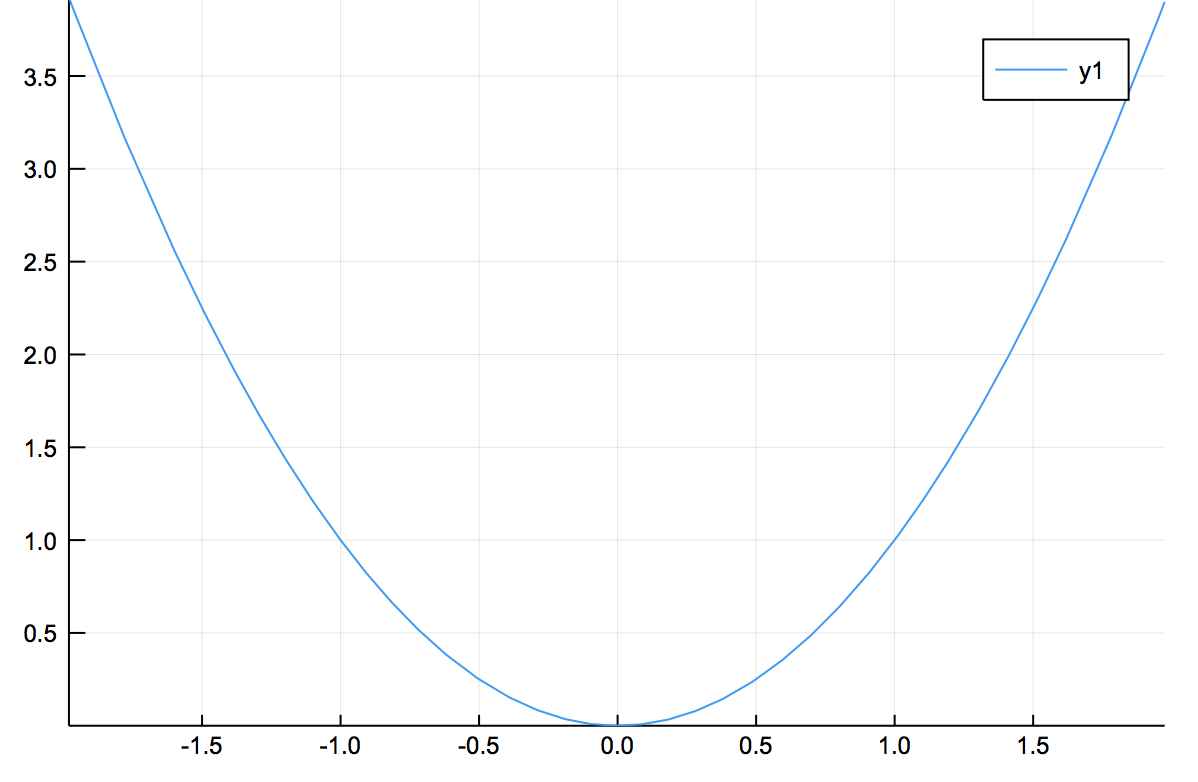
\includegraphics[width=4in]{plots/plots/plot08.png}
\end{center}

\begin{jlverbatim}
using PlotlyJS
plotlyjs()
plot(x->x^2,-2,2)
\end{jlverbatim}
%
results in:
%
\begin{center}
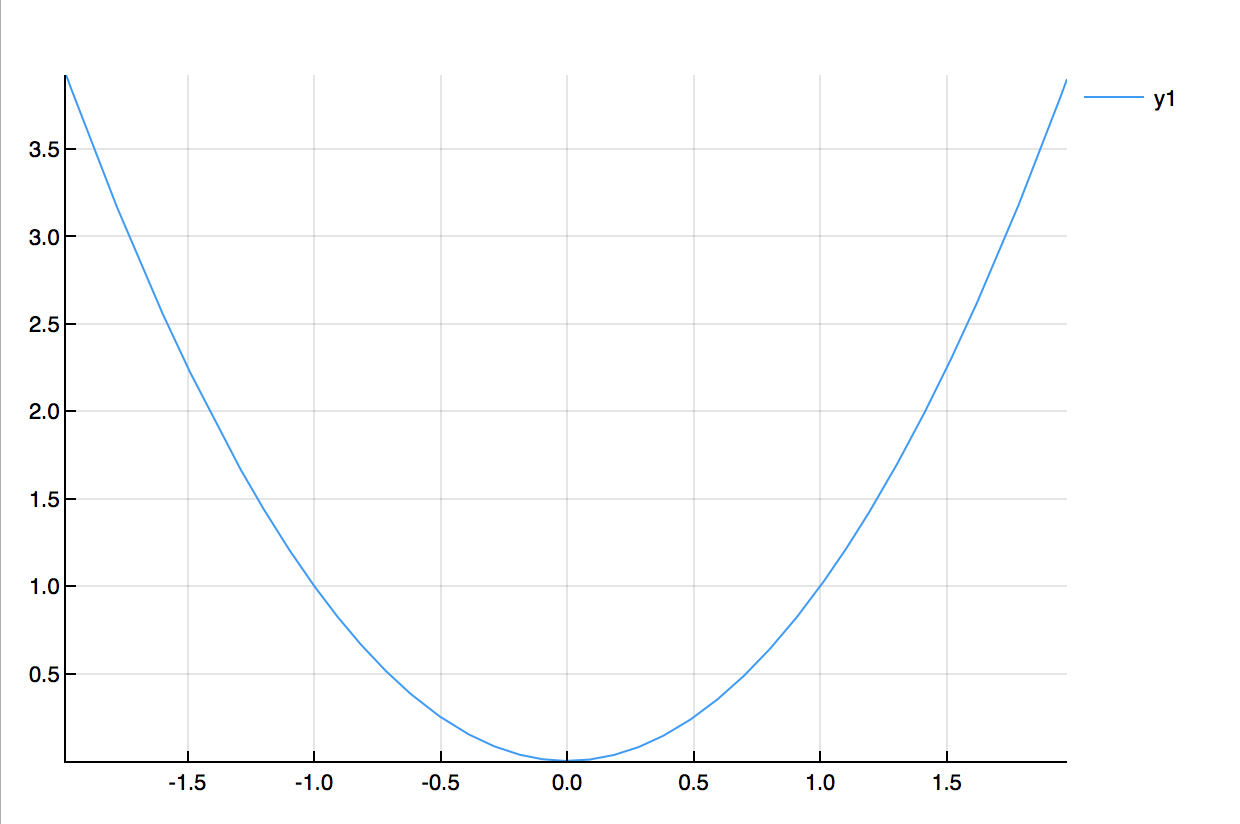
\includegraphics[width=4in]{plots/plots/plot09.png}
\end{center}
and then

\begin{jlblock}[plots]
using PGFPlotsX
pgfplotsx()
plot(x->x^2,-2,2)
\end{jlblock}
%
results in:
%
\begin{center}
\pgfplotsset{scale=0.6}
\plot{plots/plots/pgfplotsx.tex}{plots}
\end{center}
and finally
%
\begin{jlverbatim}
using PyPlot
pyplot()
plot(x->x^2,-2,2)
\end{jlverbatim}
%
results in:
%
\begin{center}
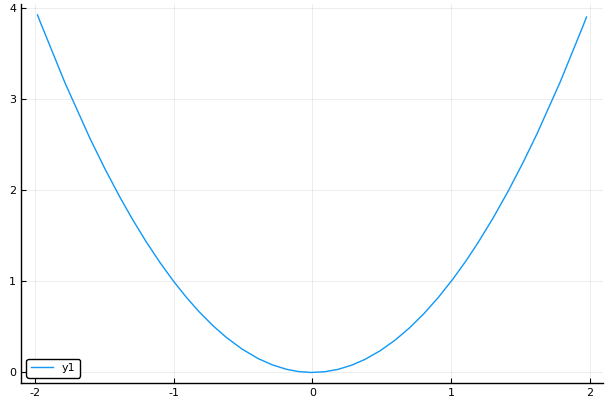
\includegraphics[width=4in]{plots/plots/plot11.png}
\end{center}

For additional information on the supported backends, visit
\href{http://docs.juliaplots.org/latest/backends/}{the Plots.jl backend
documentation}


\subsection{Changing the attributes of the plot}

Let's return back to the function plots above (although this works for
point/line plots as well) and change many attributes of the curve. As an
example:

\begin{jlblock}[plots]
plot([x->x^2,sin],-2,2,title="Two Curves",label=["x squared" "sin(x)"],xlabel="x",ylabel="y",lw=3)
\end{jlblock}

results in
%
\begin{center}
\pgfplotsset{scale=0.7}
\plot{plots/plots/attrs.tex}{plots}
\end{center}
The format is fairly clear for the changing of the attributes. Note: in
this example:

\begin{itemize}
\item  the \texttt{title} changes the title of the plot
\item  the \texttt{label} changes the legend.
\item  the \texttt{xlabel} and \texttt{ylabel} changes the axes labels.
\item  the \texttt{lw} is the line weight.
\end{itemize}

To avoid duplicating tons of documentation, visit
\href{http://docs.juliaplots.org/latest/attributes/}{the Plots.jl page
on attributes} to find all of the information to get the plot the way
you want. 

\subsection{Exercise}

\begin{itemize}

\item  Take the scatterplot above (with the random dots) and change the color
  of the dots to darkgreen, change the markers to diamonds and the size of the points 
  to about twice the default size.
\item On the function plot, make the line thicker and style to dashed. 
\end{itemize}


\section{Other plots}

\subsection{Parametric Plots}

To do a parametric plot, like the circle defined by $x(t)=\cos t, y(t)=\sin t$, then

\begin{jlblock}[plots]
plot(t->cos(t),t->sin(t),0,2*pi,legend=false)
\end{jlblock}
%
where the legend is turned off, since with one curve, it doesn't make much sense. The result is
\begin{center}
\pgfplotsset{scale=0.7}
\plot{plots/plots/parametric01.tex}{plots}
\end{center}


but notice that this should be a circle, but it looks like an ellipse
due to the aspect ratio. If one instead adds the
\verb!aspect_ratio=:equal! option, as in 
\begin{jlblock}[plots]
plot(t->cos(t),t->sin(t),0,2*pi,aspect_ratio=:equal, legend=false)
\end{jlblock}
\begin{center}
\pgfplotsset{scale=0.7}
\plot{plots/plots/parametric02.tex}{plots}
\end{center}


\subsection{Bar plots}

A bar plot can be made with the \texttt{bar} command. For example:

\begin{jlblock}[plots]
bar(1:10,y)
\end{jlblock}
where y was defined above for the scatter plot.  The result is
%
\begin{center}
\pgfplotsset{scale=0.7}
\plot{plots/plots/bar01.tex}{plots}
\end{center}


\subsection{Surface Plots}

If we have a function of 2 variables, a surface plot is nice to use. For
example, if we have the function \(f(x,y)=0.1e^{x^2+y^2}\) and we want
to plot it from -3 to 3 in both directions, if we define

\begin{jlblock}[plots]
f(x,y)=exp(-0.1*(x^2+y^2))
x = y = range(-5, stop = 5, length = 40)
\end{jlblock}
%
and then plot with
%
\begin{jlverbatim}
plot(x,y, f, st = :surface)
\end{jlverbatim}


\begin{jlcode}[plots]
pl = plot(x,y, f, st = :surface)

function cleanPreamble(preamble::String)
  lines_to_remove = r"RequirePackage|documentclass|usepackage|compat=newest|usepgfplotslibrary|^%\sDefault|usetikzlibrary"
  split(preamble,"\n") |> arr -> filter(str -> !occursin(lines_to_remove,str),arr) |> arr -> join(arr,"\n")
end

open("plots/plots/surf_preamble.tex", "w") do io
           write(io, cleanPreamble(Plots.pgfx_preamble(pl)))
       end;

\end{jlcode}


\begin{center}
\pgfplotsset{scale=0.7}
\IfFileExists{./plots/plots/surf_preamble.tex}{\input{plots/plots/surf_preamble.tex}}{}
%\plot{plots/plots/surf.tex}{plots}
{\color{red} HIDDEN PLOT}
\end{center}


\subsection{Heat maps}

Similar to above, we can make a heat map with

\begin{jlverbatim}
plot(x,y, f, st=:heatmap)
\end{jlverbatim}

\begin{jlcode}[plots]
pl = plot(x,y, f, st=:heatmap)

open("plots/plots/heat_preamble.tex", "w") do io
           write(io, cleanPreamble(Plots.pgfx_preamble(pl)))
       end;
\end{jlcode}
%
which produces
%
\begin{center}
\pgfplotsset{scale=0.7}
\IfFileExists{./plots/plots/heat_preamble.tex}{\pgfplotsset{%
layers/standard/.define layer set={%
    background,axis background,axis grid,axis ticks,axis lines,axis tick labels,pre main,main,axis descriptions,axis foreground%
}{grid style= {/pgfplots/on layer=axis grid},%
    tick style= {/pgfplots/on layer=axis ticks},%
    axis line style= {/pgfplots/on layer=axis lines},%
    label style= {/pgfplots/on layer=axis descriptions},%
    legend style= {/pgfplots/on layer=axis descriptions},%
    title style= {/pgfplots/on layer=axis descriptions},%
    colorbar style= {/pgfplots/on layer=axis descriptions},%
    ticklabel style= {/pgfplots/on layer=axis tick labels},%
    axis background@ style={/pgfplots/on layer=axis background},%
    3d box foreground style={/pgfplots/on layer=axis foreground},%
    },
}

\pgfplotsset{
colormap={plots1}{rgb(0.00000000cm)=(0.00146200,0.00046600,0.01386600)
rgb(0.00392157cm)=(0.00226700,0.00127000,0.01857000)
rgb(0.00784314cm)=(0.00329900,0.00224900,0.02423900)
rgb(0.01176471cm)=(0.00454700,0.00339200,0.03090900)
rgb(0.01568627cm)=(0.00600600,0.00469200,0.03855800)
rgb(0.01960784cm)=(0.00767600,0.00613600,0.04683600)
rgb(0.02352941cm)=(0.00956100,0.00771300,0.05514300)
rgb(0.02745098cm)=(0.01166300,0.00941700,0.06346000)
rgb(0.03137255cm)=(0.01399500,0.01122500,0.07186200)
rgb(0.03529412cm)=(0.01656100,0.01313600,0.08028200)
rgb(0.03921569cm)=(0.01937300,0.01513300,0.08876700)
rgb(0.04313725cm)=(0.02244700,0.01719900,0.09732700)
rgb(0.04705882cm)=(0.02579300,0.01933100,0.10593000)
rgb(0.05098039cm)=(0.02943200,0.02150300,0.11462100)
rgb(0.05490196cm)=(0.03338500,0.02370200,0.12339700)
rgb(0.05882353cm)=(0.03766800,0.02592100,0.13223200)
rgb(0.06274510cm)=(0.04225300,0.02813900,0.14114100)
rgb(0.06666667cm)=(0.04691500,0.03032400,0.15016400)
rgb(0.07058824cm)=(0.05164400,0.03247400,0.15925400)
rgb(0.07450980cm)=(0.05644900,0.03456900,0.16841400)
rgb(0.07843137cm)=(0.06134000,0.03659000,0.17764200)
rgb(0.08235294cm)=(0.06633100,0.03850400,0.18696200)
rgb(0.08627451cm)=(0.07142900,0.04029400,0.19635400)
rgb(0.09019608cm)=(0.07663700,0.04190500,0.20579900)
rgb(0.09411765cm)=(0.08196200,0.04332800,0.21528900)
rgb(0.09803922cm)=(0.08741100,0.04455600,0.22481300)
rgb(0.10196078cm)=(0.09299000,0.04558300,0.23435800)
rgb(0.10588235cm)=(0.09870200,0.04640200,0.24390400)
rgb(0.10980392cm)=(0.10455100,0.04700800,0.25343000)
rgb(0.11372549cm)=(0.11053600,0.04739900,0.26291200)
rgb(0.11764706cm)=(0.11665600,0.04757400,0.27232100)
rgb(0.12156863cm)=(0.12290800,0.04753600,0.28162400)
rgb(0.12549020cm)=(0.12928500,0.04729300,0.29078800)
rgb(0.12941176cm)=(0.13577800,0.04685600,0.29977600)
rgb(0.13333333cm)=(0.14237800,0.04624200,0.30855300)
rgb(0.13725490cm)=(0.14907300,0.04546800,0.31708500)
rgb(0.14117647cm)=(0.15585000,0.04455900,0.32533800)
rgb(0.14509804cm)=(0.16268900,0.04355400,0.33327700)
rgb(0.14901961cm)=(0.16957500,0.04248900,0.34087400)
rgb(0.15294118cm)=(0.17649300,0.04140200,0.34811100)
rgb(0.15686275cm)=(0.18342900,0.04032900,0.35497100)
rgb(0.16078431cm)=(0.19036700,0.03930900,0.36144700)
rgb(0.16470588cm)=(0.19729700,0.03840000,0.36753500)
rgb(0.16862745cm)=(0.20420900,0.03763200,0.37323800)
rgb(0.17254902cm)=(0.21109500,0.03703000,0.37856300)
rgb(0.17647059cm)=(0.21794900,0.03661500,0.38352200)
rgb(0.18039216cm)=(0.22476300,0.03640500,0.38812900)
rgb(0.18431373cm)=(0.23153800,0.03640500,0.39240000)
rgb(0.18823529cm)=(0.23827300,0.03662100,0.39635300)
rgb(0.19215686cm)=(0.24496700,0.03705500,0.40000700)
rgb(0.19607843cm)=(0.25162000,0.03770500,0.40337800)
rgb(0.20000000cm)=(0.25823400,0.03857100,0.40648500)
rgb(0.20392157cm)=(0.26481000,0.03964700,0.40934500)
rgb(0.20784314cm)=(0.27134700,0.04092200,0.41197600)
rgb(0.21176471cm)=(0.27785000,0.04235300,0.41439200)
rgb(0.21568627cm)=(0.28432100,0.04393300,0.41660800)
rgb(0.21960784cm)=(0.29076300,0.04564400,0.41863700)
rgb(0.22352941cm)=(0.29717800,0.04747000,0.42049100)
rgb(0.22745098cm)=(0.30356800,0.04939600,0.42218200)
rgb(0.23137255cm)=(0.30993500,0.05140700,0.42372100)
rgb(0.23529412cm)=(0.31628200,0.05349000,0.42511600)
rgb(0.23921569cm)=(0.32261000,0.05563400,0.42637700)
rgb(0.24313725cm)=(0.32892100,0.05782700,0.42751100)
rgb(0.24705882cm)=(0.33521700,0.06006000,0.42852400)
rgb(0.25098039cm)=(0.34150000,0.06232500,0.42942500)
rgb(0.25490196cm)=(0.34777100,0.06461600,0.43021700)
rgb(0.25882353cm)=(0.35403200,0.06692500,0.43090600)
rgb(0.26274510cm)=(0.36028400,0.06924700,0.43149700)
rgb(0.26666667cm)=(0.36652900,0.07157900,0.43199400)
rgb(0.27058824cm)=(0.37276800,0.07391500,0.43240000)
rgb(0.27450980cm)=(0.37900100,0.07625300,0.43271900)
rgb(0.27843137cm)=(0.38522800,0.07859100,0.43295500)
rgb(0.28235294cm)=(0.39145300,0.08092700,0.43310900)
rgb(0.28627451cm)=(0.39767400,0.08325700,0.43318300)
rgb(0.29019608cm)=(0.40389400,0.08558000,0.43317900)
rgb(0.29411765cm)=(0.41011300,0.08789600,0.43309800)
rgb(0.29803922cm)=(0.41633100,0.09020300,0.43294300)
rgb(0.30196078cm)=(0.42254900,0.09250100,0.43271400)
rgb(0.30588235cm)=(0.42876800,0.09479000,0.43241200)
rgb(0.30980392cm)=(0.43498700,0.09706900,0.43203900)
rgb(0.31372549cm)=(0.44120700,0.09933800,0.43159400)
rgb(0.31764706cm)=(0.44742800,0.10159700,0.43108000)
rgb(0.32156863cm)=(0.45365100,0.10384800,0.43049800)
rgb(0.32549020cm)=(0.45987500,0.10608900,0.42984600)
rgb(0.32941176cm)=(0.46610000,0.10832200,0.42912500)
rgb(0.33333333cm)=(0.47232800,0.11054700,0.42833400)
rgb(0.33725490cm)=(0.47855800,0.11276400,0.42747500)
rgb(0.34117647cm)=(0.48478900,0.11497400,0.42654800)
rgb(0.34509804cm)=(0.49102200,0.11717900,0.42555200)
rgb(0.34901961cm)=(0.49725700,0.11937900,0.42448800)
rgb(0.35294118cm)=(0.50349300,0.12157500,0.42335600)
rgb(0.35686275cm)=(0.50973000,0.12376900,0.42215600)
rgb(0.36078431cm)=(0.51596700,0.12596000,0.42088700)
rgb(0.36470588cm)=(0.52220600,0.12815000,0.41954900)
rgb(0.36862745cm)=(0.52844400,0.13034100,0.41814200)
rgb(0.37254902cm)=(0.53468300,0.13253400,0.41666700)
rgb(0.37647059cm)=(0.54092000,0.13472900,0.41512300)
rgb(0.38039216cm)=(0.54715700,0.13692900,0.41351100)
rgb(0.38431373cm)=(0.55339200,0.13913400,0.41182900)
rgb(0.38823529cm)=(0.55962400,0.14134600,0.41007800)
rgb(0.39215686cm)=(0.56585400,0.14356700,0.40825800)
rgb(0.39607843cm)=(0.57208100,0.14579700,0.40636900)
rgb(0.40000000cm)=(0.57830400,0.14803900,0.40441100)
rgb(0.40392157cm)=(0.58452100,0.15029400,0.40238500)
rgb(0.40784314cm)=(0.59073400,0.15256300,0.40029000)
rgb(0.41176471cm)=(0.59694000,0.15484800,0.39812500)
rgb(0.41568627cm)=(0.60313900,0.15715100,0.39589100)
rgb(0.41960784cm)=(0.60933000,0.15947400,0.39358900)
rgb(0.42352941cm)=(0.61551300,0.16181700,0.39121900)
rgb(0.42745098cm)=(0.62168500,0.16418400,0.38878100)
rgb(0.43137255cm)=(0.62784700,0.16657500,0.38627600)
rgb(0.43529412cm)=(0.63399800,0.16899200,0.38370400)
rgb(0.43921569cm)=(0.64013500,0.17143800,0.38106500)
rgb(0.44313725cm)=(0.64626000,0.17391400,0.37835900)
rgb(0.44705882cm)=(0.65236900,0.17642100,0.37558600)
rgb(0.45098039cm)=(0.65846300,0.17896200,0.37274800)
rgb(0.45490196cm)=(0.66454000,0.18153900,0.36984600)
rgb(0.45882353cm)=(0.67059900,0.18415300,0.36687900)
rgb(0.46274510cm)=(0.67663800,0.18680700,0.36384900)
rgb(0.46666667cm)=(0.68265600,0.18950100,0.36075700)
rgb(0.47058824cm)=(0.68865300,0.19223900,0.35760300)
rgb(0.47450980cm)=(0.69462700,0.19502100,0.35438800)
rgb(0.47843137cm)=(0.70057600,0.19785100,0.35111300)
rgb(0.48235294cm)=(0.70650000,0.20072800,0.34777700)
rgb(0.48627451cm)=(0.71239600,0.20365600,0.34438300)
rgb(0.49019608cm)=(0.71826400,0.20663600,0.34093100)
rgb(0.49411765cm)=(0.72410300,0.20967000,0.33742400)
rgb(0.49803922cm)=(0.72990900,0.21275900,0.33386100)
rgb(0.50196078cm)=(0.73568300,0.21590600,0.33024500)
rgb(0.50588235cm)=(0.74142300,0.21911200,0.32657600)
rgb(0.50980392cm)=(0.74712700,0.22237800,0.32285600)
rgb(0.51372549cm)=(0.75279400,0.22570600,0.31908500)
rgb(0.51764706cm)=(0.75842200,0.22909700,0.31526600)
rgb(0.52156863cm)=(0.76401000,0.23255400,0.31139900)
rgb(0.52549020cm)=(0.76955600,0.23607700,0.30748500)
rgb(0.52941176cm)=(0.77505900,0.23966700,0.30352600)
rgb(0.53333333cm)=(0.78051700,0.24332700,0.29952300)
rgb(0.53725490cm)=(0.78592900,0.24705600,0.29547700)
rgb(0.54117647cm)=(0.79129300,0.25085600,0.29139000)
rgb(0.54509804cm)=(0.79660700,0.25472800,0.28726400)
rgb(0.54901961cm)=(0.80187100,0.25867400,0.28309900)
rgb(0.55294118cm)=(0.80708200,0.26269200,0.27889800)
rgb(0.55686275cm)=(0.81223900,0.26678600,0.27466100)
rgb(0.56078431cm)=(0.81734100,0.27095400,0.27039000)
rgb(0.56470588cm)=(0.82238600,0.27519700,0.26608500)
rgb(0.56862745cm)=(0.82737200,0.27951700,0.26175000)
rgb(0.57254902cm)=(0.83229900,0.28391300,0.25738300)
rgb(0.57647059cm)=(0.83716500,0.28838500,0.25298800)
rgb(0.58039216cm)=(0.84196900,0.29293300,0.24856400)
rgb(0.58431373cm)=(0.84670900,0.29755900,0.24411300)
rgb(0.58823529cm)=(0.85138400,0.30226000,0.23963600)
rgb(0.59215686cm)=(0.85599200,0.30703800,0.23513300)
rgb(0.59607843cm)=(0.86053300,0.31189200,0.23060600)
rgb(0.60000000cm)=(0.86500600,0.31682200,0.22605500)
rgb(0.60392157cm)=(0.86940900,0.32182700,0.22148200)
rgb(0.60784314cm)=(0.87374100,0.32690600,0.21688600)
rgb(0.61176471cm)=(0.87800100,0.33206000,0.21226800)
rgb(0.61568627cm)=(0.88218800,0.33728700,0.20762800)
rgb(0.61960784cm)=(0.88630200,0.34258600,0.20296800)
rgb(0.62352941cm)=(0.89034100,0.34795700,0.19828600)
rgb(0.62745098cm)=(0.89430500,0.35339900,0.19358400)
rgb(0.63137255cm)=(0.89819200,0.35891100,0.18886000)
rgb(0.63529412cm)=(0.90200300,0.36449200,0.18411600)
rgb(0.63921569cm)=(0.90573500,0.37014000,0.17935000)
rgb(0.64313725cm)=(0.90939000,0.37585600,0.17456300)
rgb(0.64705882cm)=(0.91296600,0.38163600,0.16975500)
rgb(0.65098039cm)=(0.91646200,0.38748100,0.16492400)
rgb(0.65490196cm)=(0.91987900,0.39338900,0.16007000)
rgb(0.65882353cm)=(0.92321500,0.39935900,0.15519300)
rgb(0.66274510cm)=(0.92647000,0.40538900,0.15029200)
rgb(0.66666667cm)=(0.92964400,0.41147900,0.14536700)
rgb(0.67058824cm)=(0.93273700,0.41762700,0.14041700)
rgb(0.67450980cm)=(0.93574700,0.42383100,0.13544000)
rgb(0.67843137cm)=(0.93867500,0.43009100,0.13043800)
rgb(0.68235294cm)=(0.94152100,0.43640500,0.12540900)
rgb(0.68627451cm)=(0.94428500,0.44277200,0.12035400)
rgb(0.69019608cm)=(0.94696500,0.44919100,0.11527200)
rgb(0.69411765cm)=(0.94956200,0.45566000,0.11016400)
rgb(0.69803922cm)=(0.95207500,0.46217800,0.10503100)
rgb(0.70196078cm)=(0.95450600,0.46874400,0.09987400)
rgb(0.70588235cm)=(0.95685200,0.47535600,0.09469500)
rgb(0.70980392cm)=(0.95911400,0.48201400,0.08949900)
rgb(0.71372549cm)=(0.96129300,0.48871600,0.08428900)
rgb(0.71764706cm)=(0.96338700,0.49546200,0.07907300)
rgb(0.72156863cm)=(0.96539700,0.50224900,0.07385900)
rgb(0.72549020cm)=(0.96732200,0.50907800,0.06865900)
rgb(0.72941176cm)=(0.96916300,0.51594600,0.06348800)
rgb(0.73333333cm)=(0.97091900,0.52285300,0.05836700)
rgb(0.73725490cm)=(0.97259000,0.52979800,0.05332400)
rgb(0.74117647cm)=(0.97417600,0.53678000,0.04839200)
rgb(0.74509804cm)=(0.97567700,0.54379800,0.04361800)
rgb(0.74901961cm)=(0.97709200,0.55085000,0.03905000)
rgb(0.75294118cm)=(0.97842200,0.55793700,0.03493100)
rgb(0.75686275cm)=(0.97966600,0.56505700,0.03140900)
rgb(0.76078431cm)=(0.98082400,0.57220900,0.02850800)
rgb(0.76470588cm)=(0.98189500,0.57939200,0.02625000)
rgb(0.76862745cm)=(0.98288100,0.58660600,0.02466100)
rgb(0.77254902cm)=(0.98377900,0.59384900,0.02377000)
rgb(0.77647059cm)=(0.98459100,0.60112200,0.02360600)
rgb(0.78039216cm)=(0.98531500,0.60842200,0.02420200)
rgb(0.78431373cm)=(0.98595200,0.61575000,0.02559200)
rgb(0.78823529cm)=(0.98650200,0.62310500,0.02781400)
rgb(0.79215686cm)=(0.98696400,0.63048500,0.03090800)
rgb(0.79607843cm)=(0.98733700,0.63789000,0.03491600)
rgb(0.80000000cm)=(0.98762200,0.64532000,0.03988600)
rgb(0.80392157cm)=(0.98781900,0.65277300,0.04558100)
rgb(0.80784314cm)=(0.98792600,0.66025000,0.05175000)
rgb(0.81176471cm)=(0.98794500,0.66774800,0.05832900)
rgb(0.81568627cm)=(0.98787400,0.67526700,0.06525700)
rgb(0.81960784cm)=(0.98771400,0.68280700,0.07248900)
rgb(0.82352941cm)=(0.98746400,0.69036600,0.07999000)
rgb(0.82745098cm)=(0.98712400,0.69794400,0.08773100)
rgb(0.83137255cm)=(0.98669400,0.70554000,0.09569400)
rgb(0.83529412cm)=(0.98617500,0.71315300,0.10386300)
rgb(0.83921569cm)=(0.98556600,0.72078200,0.11222900)
rgb(0.84313725cm)=(0.98486500,0.72842700,0.12078500)
rgb(0.84705882cm)=(0.98407500,0.73608700,0.12952700)
rgb(0.85098039cm)=(0.98319600,0.74375800,0.13845300)
rgb(0.85490196cm)=(0.98222800,0.75144200,0.14756500)
rgb(0.85882353cm)=(0.98117300,0.75913500,0.15686300)
rgb(0.86274510cm)=(0.98003200,0.76683700,0.16635300)
rgb(0.86666667cm)=(0.97880600,0.77454500,0.17603700)
rgb(0.87058824cm)=(0.97749700,0.78225800,0.18592300)
rgb(0.87450980cm)=(0.97610800,0.78997400,0.19601800)
rgb(0.87843137cm)=(0.97463800,0.79769200,0.20633200)
rgb(0.88235294cm)=(0.97308800,0.80540900,0.21687700)
rgb(0.88627451cm)=(0.97146800,0.81312200,0.22765800)
rgb(0.89019608cm)=(0.96978300,0.82082500,0.23868600)
rgb(0.89411765cm)=(0.96804100,0.82851500,0.24997200)
rgb(0.89803922cm)=(0.96624300,0.83619100,0.26153400)
rgb(0.90196078cm)=(0.96439400,0.84384800,0.27339100)
rgb(0.90588235cm)=(0.96251700,0.85147600,0.28554600)
rgb(0.90980392cm)=(0.96062600,0.85906900,0.29801000)
rgb(0.91372549cm)=(0.95872000,0.86662400,0.31082000)
rgb(0.91764706cm)=(0.95683400,0.87412900,0.32397400)
rgb(0.92156863cm)=(0.95499700,0.88156900,0.33747500)
rgb(0.92549020cm)=(0.95321500,0.88894200,0.35136900)
rgb(0.92941176cm)=(0.95154600,0.89622600,0.36562700)
rgb(0.93333333cm)=(0.95001800,0.90340900,0.38027100)
rgb(0.93725490cm)=(0.94868300,0.91047300,0.39528900)
rgb(0.94117647cm)=(0.94759400,0.91739900,0.41066500)
rgb(0.94509804cm)=(0.94680900,0.92416800,0.42637300)
rgb(0.94901961cm)=(0.94639200,0.93076100,0.44236700)
rgb(0.95294118cm)=(0.94640300,0.93715900,0.45859200)
rgb(0.95686275cm)=(0.94690300,0.94334800,0.47497000)
rgb(0.96078431cm)=(0.94793700,0.94931800,0.49142600)
rgb(0.96470588cm)=(0.94954500,0.95506300,0.50786000)
rgb(0.96862745cm)=(0.95174000,0.96058700,0.52420300)
rgb(0.97254902cm)=(0.95452900,0.96589600,0.54036100)
rgb(0.97647059cm)=(0.95789600,0.97100300,0.55627500)
rgb(0.98039216cm)=(0.96181200,0.97592400,0.57192500)
rgb(0.98431373cm)=(0.96624900,0.98067800,0.58720600)
rgb(0.98823529cm)=(0.97116200,0.98528200,0.60215400)
rgb(0.99215686cm)=(0.97651100,0.98975300,0.61676000)
rgb(0.99607843cm)=(0.98225700,0.99410900,0.63101700)
rgb(1.00000000cm)=(0.98836200,0.99836400,0.64492400)},
}
}{}
%\plot{plots/plots/heat.tex}{plots}
{\color{red} HIDDEN PLOT}
\end{center}


\subsection{Animation}

Another nice type of plot under Plots.jl is that of an animation,
however you will need to have \texttt{ffmpeg} installed on your machine.
If you then do

\begin{jlverbatim}
@gif for a in range(0.5,stop=2,length=16)
  plot(t->cos(2t),t->sin(a*t),0,2pi,legend=false)
end
\end{jlverbatim}

which saves to a gif that the output will describe this results in:



\section{Other Plots and subplots}

This just is the tip of the iceberg for plotting. Take a look at the
\href{http://docs.juliaplots.org/latest/}{Plots.jl documentation} or do
some google-foo with the phrase `Plots.jl' and what you're looking for
and good spot for Q\&A is
\href{https://discourse.julialang.org/c/domain/viz}{a julialang.org
discourse site}

\section{Exercises}

Use the plotting techniques in this section to plot the following.  For each, hide the legend when ther e is only one curve/set of data and label appropriate if more than one curve/set of data.  Include a title as well. 

\begin{enumerate}
\item The function $y=e^{-x^2}$ from $x=-3$ to $x=3$
\item The functions $y=\sin x, y=\sin 2x, y=\sin 3$ from $x=-\pi$ to $x=\pi$. 
\item A scatter plot of the following:
\begin{center}
\begin{tabular}{r|rrrrrrrrrrrrrr}
$x$ & 0 & 2 & 3 & 4 & 6 & 9 & 10 & 11 & 13 & 15 & 16 & 18 & 20 \\
$y$ & $-1$ & 4 & 3 & 6 & 2 & 0 & 2 & 9 & 5 & $-2$ & 4 & 6 & 3\\
\end{tabular}
\end{center}
\item A surface plot of $z=\sin(x-y)$ with $0 \leq x \leq \pi, 0 \leq y \leq \pi$.
\item A heat map of $z=\sin(x-y)$ with $0 \leq x \leq \pi, 0 \leq y \leq \pi$.
\end{enumerate}

% !TEX encoding = UTF-8 Unicode
% !TEX root = scientific-computing.tex
%

\chapter{Creating New Data Types in Julia}\label{ch:comp-types}

Although there are many standard Julia data types that are useful for Scientific Computing, we can make new types called a composite data type.  We will start with developing a \texttt{PlayingCard} type that simplifies the poker hand simulations that we will see in Chapter \ref{ch:poker}.  We will also look at a \texttt{Polynomial} data type and finally create a \texttt{Root} type that will help with the rootfinding from Chapter \ref{ch:rootfinding}.

\section{Basics of Julia's Composite Datatype} 

The composite data type in Julia is called a \texttt{struct} and consists of some number of fields of an existing type.  A simple one is 
\begin{jlblock}[newtype]
struct Mystruct
  num::Integer
  str::String
end
\end{jlblock}
%
which has the two fields \texttt{num} and \texttt{str}. We are using the standard naming convention of a struct starting with a capital letter.  We can create an object\footnote{Although a Julia struct is not an object in the sense of an object-oriented language, the terminology is pervasive in the Julia community.} of type \texttt{Mystruct} by
% 
\begin{jlblock}[newtype]
m = Mystruct(13,"hello")
\end{jlblock}
and we can access the fields of the struct with \texttt{m.num} and \texttt{m.str}.  They will return \jlc[newtype]{print(m.num)} \printpythontex[verb]~ and \jlc[newtype]{print(m.str)} \printpythontex[verb].   Also, you can get an array of the names of the fields with \jlb[newtype]{fieldnames(Mystruct)}.  Note that the \texttt{fieldnames} command needs the datatype, not a variable of the datatype. This example is not very realistic, but the rest of the chapter will include more-practical examples. 

One cannot change the fields of a \texttt{struct}.  If \texttt{m} is defined as above and you try
\begin{jlcode}[newtype-err]
struct Mystruct
  num::Integer
  str::String
end
m=Mystruct(13,"hello")
\end{jlcode}

\begin{jlverbatim}[newtype-err]
m.str = "goodbye"
\end{jlverbatim}
\begin{jlcode}[newtype-err]
try
  m.str = "goodbye"
catch e
 printstyled(stderr,"ERROR: ", bold=true, color=:red)
 printstyled(stderr,sprint(showerror,e), color=:light_red)
 println(stderr)
end
\end{jlcode}
%
%\stderrpythontex
%
then Julia will report the error:
\stderrpythontex[verbatim]

This is exactly like trying to redefine a \texttt{const}.  As we will see most of the examples in this text are these constant types of \texttt{struct}s, you can make non-constant \texttt{structs} using the \texttt{mutable} keyword.  For example:
%
\begin{jlblock}[newtype]
mutable struct MutableStruct
  a::Float64
  b::Integer
end
\end{jlblock}
%
and then define an object such as
\begin{jlblock}[newtype]
s=MutableStruct(1,2)
\end{jlblock}
%
Then the redefinition \jlb[newtype]{s.a=4.5} is allowed.  Note: that if you try to do \jlv[newtype]{s.b=7.1}, the you will get the error:
\begin{jlcode}[newtype2]
mutable struct MutableStruct
  a::Float64
  b::Integer
end
s=MutableStruct(1,2)
try
  s.b = 7.1
catch e
 printstyled(stderr,"ERROR: ", bold=true, color=:red)
 printstyled(stderr,sprint(showerror,e), color=:light_red)
 println(stderr)
end
\end{jlcode}
\stderrpythontex[verbatim]
%
which happens because you are trying to assign the value 7.1 to an integer, since the field \texttt{b} is an integer.    


\section{A Card datatype}

In Chapter \ref{ch:poker}, we will use simulations to determine the probabilities of certain poker hands. Although the calculations can be done with built-in types, the result would be difficult to read and hard to understand.  Here, we will create a \texttt{Card} datatype that will help clarify the code by creating a type with a rank (1 to 13 corresponding to Ace, 2, through 10, Jack, Queen, King) and a suit (1 to 4 corresponding to the suits ``spades'', ``hearts'', ``diamonds'', ``clubs''), which we define as the characters arrays:
%
\begin{jlblock}[newtype2]
ranks = ['A','2','3','4','5','6','7','8','9','T','J','Q','K'];
suits = ['\u2660','\u2661','\u2662','\u2663']
\end{jlblock}
\begin{jlcode}[newtype]
ranks = ['A','2','3','4','5','6','7','8','9','T','J','Q','K'];
suits = ['\u2660','\u2661','\u2662','\u2663']
\end{jlcode}

%
where the suits are the unicode characters for the suits. See
\href{http://docs.julialang.org/en/latest/manual/unicode-input/}{the
julia documentation on unicode}. We will create the following datatype:
\begin{jlblock}[newtype2]
struct Card
    rank::Integer
    suit::Integer
end
\end{jlblock}
%
and if we enter \jlb[newtype2]{c = Card(3,2)}, then this will create a card of rank 3 and suit 2 (hearts). To access the fields of the type, we use dot notation. For example \jlb[newtype2]{c.rank}
will return \jlc[newtype2]{print(c.rank)} \printpythontex[verb] ~and \jlb[newtype2]{c.suit} will return \jlc[newtype2]{print(c.suit)} \printpythontex[verb]. 

Julia allows the printing of any type of data in a specified way.  To do this we will define \texttt{Base.show} for our type. To do this, enter
\begin{jlblock}[newtype2]
Base.show(io::IO, c::Card) = print(io, string(ranks[c.rank],suits[c.suit]))
\end{jlblock}
%
where the arguments of \texttt{Base.show} should be of type \texttt{IO}
and then a print should be called as above. The result will be the concatenation of the characters corresponding to the rank and suit of the card.  Try this out by typing \jlb[newtype2]{c} and you should get \jlc[newtype2]{print(c)} \printpythontex[verb]. 


Note: this is different than just a \texttt{print} or \texttt{println} within a function, which is highly discouraged. This function is called whenever a card type is displayed. 

When julia calls \texttt{Card(3,2)}, actually, it executes a special function called a constructor, which creates an instance of the type, which we have called an object. Although Julia creates the basic constructor--that is the one that fills the fields of the type in the order defined, we may want another constructor that will take an integer between 1 and 52 and returns the appropriate card. The following example
will do this.

\begin{jlblock}[newtype][numbers=left]
struct Card
  rank::Int
  suit::Int
  Card(r::Int,s::Int)=(1<=r<=13) ? ( (1<=s<=4) ? new(r,s) :
    throw(ArgumentError("The argument for suit must be between 1 and 4")) ) :
	throw(ArgumentError("The argument for rank must be between 1 and 13")) 
  Card(i::Int) = !(1<=i<=52) ? 
    throw(ArgumentError("The argument must be an integer between 1 and 52")) : 
    i%13==0 ? new(13,div(i,13)) : new(i%13,div(i,13)+1)
end
\end{jlblock}
\begin{jlcode}[newtype]
Base.show(io::IO, c::Card) = print(io, string(ranks[c.rank],suits[c.suit]))
\end{jlcode}

There are a number of things about this definition:
\begin{itemize}
\item It is still a struct with two members (rank and suit)
\item There is a function \jlv{new} used.  This will use the default constructors that is \jlv{new(3,4)} would define rank to be 3 and suit to be 4. 
\item The lines 4--6 define a Card with the two arguments.  However, it tests to make sure that you put in valid ranks and suits.  This is a bit complicated in that there is a nested tenary \verb!if-then-else! command. 
\item The lines 7--9 define the constructor that takes a single integer and checks if that is valid. It uses integer division and the modulo \verb!%! to calculate the rank and suit.  
\end{itemize}


Notice that there is a function \texttt{new} that is called. The first
constructor is the default constructor. If a second one is made (as is
in this example), you need to explicitly define the standard constructor as well. See
\href{https://docs.julialang.org/en/latest/manual/constructors/\#man-constructors-1}{additional
information about constructors in the Julia Documentation}.

If you enter the above \texttt{struct} we saw the error:
\begin{jlverbatim}
invalid redefinition of constant Card
\end{jlverbatim}
Recall, from the beginning of this chapter, this is because a \texttt{struct} is fixed, much like if a constant is declared and then it is redefined.  We want to replace the first \texttt{struct} with this one, so we will restart the kernel by selecting \emph{kernel} in Jupyter and then select \emph{restart kernel}\footnote{In Chapter \ref{ch:modules} we will put structs in a separate file as a module and use a package called \texttt{Revise} to automatically handle changes without these errors.}.  You will need to reenter all of the needed cells, like the one with the ranks and suits as well as the one that starts \texttt{Base.show}.  In Chapter \ref{ch:modules}, we will put structs inside a module and not have to restart the kernel as you develop a new datatype.   

The second constructor will create a card from a number between 1 and 52 (and throw an error if it is not in this range). We can now create a card from an integer. For example \jlv{c1=Card(45)} will return  \jlc[newtype]{print(Card(45))} \printpythontex[verb]. 

As we will see in Chapter \ref{ch:poker}, a hand is also helpful in playing card games, we will define a hand in the following way:
%
\begin{jlblock}[newtype]
struct Hand
    cards::Array{Card,1}
end
\end{jlblock}
%
which is just an array of cards. (Note: there is nothing here that
specifies that the Hand has to be 5 cards, but that could be included by
doing some error checking in the constructor).  An example hand would be 
%
\begin{jlblock}[newtype]
h1=Hand([Card(2,3),Card(12,1),Card(10,1),Card(10,4),Card(5,2)])
\end{jlblock}
%
and again, since this looks a bit ugly, we can define a \verb!Base.show! method
for a hand:
%
\begin{jlblock}[newtype]
Base.show(io::IO,h::Hand) = print(io, string("[",join(h.cards,", "),"]"))
\end{jlblock}
\begin{jlcode}[newtype]
h1=Hand([Card(2,3),Card(12,1),Card(10,1),Card(10,4),Card(5,2)])
\end{jlcode}
%
now \texttt{h1} should now return \jlc[newtype]{display(h1)} \printpythontex[verbatim]

We will return to this in Chapter \ref{ch:poker} where we will use this datatype to help with simulations.  


\section{Polynomials--A parametric data type}\label{sect:parametric-types}

Recall that a polynomial is the sum of nonnegative powers of $x$ with constant coefficients.  That is anything of the form:
\begin{align*}
P(x) & = a_0 + a_1 x + a_2 x^2 + \cdots + a_n x^n 
\end{align*}
and we may want to solve problems with them and it may be helpful to have a data type of this form.  We can represent any polynomial by the coefficients.  For example, the following will construct a datatype that is a polynomial with integer coefficients\footnote{As well will see in Chapter \ref{ch:lin-alg-intro}, a \texttt{Vector} is shorthand or an alias for a 1D array}: 
\begin{jlverbatim}[poly]
struct Polynomial
  coeffs::Vector{Int64}
end
\end{jlverbatim}

We can then represent the polynomial $P(x) = 2-x+3x^2$ with
\begin{jlverbatim}[poly]
p = Polynomial([2,-1,3])
\end{jlverbatim}

Let's say that we want to construct methods to add, subtract, scalar multiply and plot polynomials.  However, if we want to allow Polynomials with coefficients other than integer coefficients, such as rational or real or complex, then we would need to write a set of functions to do this for each datatype, which is 1) painfully dull, 2) hard to maintain since there are many copies of the same function and 3) unnecessary because Julia has a nice feature called a parametric type. 

We could define the Polynomial as 
\begin{jlverbatim}[poly]
struct Polynomial{T}
  coeffs:Vector{T}
end
\end{jlverbatim}
%
which has Polynomial that has a type \verb!T!. This now allows with one definition to have a polynomial of integers, floats, complex and rationals.  However, this would also allow us to define a polynomial of strings or \texttt{Card}s, which doesn't make any sense.  We can restrict the coefficients to number types with 
%
\begin{jlblock}[poly]
struct Polynomial{T <: Number}
  coeffs::Vector{T}
end
\end{jlblock}
%
which allows the coefficient to be any type that is a subtype of \texttt{Number}, which is what the notation \texttt{ <: Number} means.  This defines \texttt{T} to be any type that is a Number\footnote{Recall that Chapter \ref{ch:data-types} explain the data typing system and how to determine subtypes of a type.}.  

For example, using the above definition of \texttt{Polynomial}, we can define the following
%
\begin{jlblock}[poly]
poly1=Polynomial([1,2,3])
poly2=Polynomial([1.0,2.0,3.0])
poly3=Polynomial([2//3,3//4,5//8])
poly4=Polynomial([im,2+0im,3-2im,-im])
poly5=Polynomial([n for n=1:6])
\end{jlblock}
%
and the result of the last will be \jlc[poly]{print(poly5)} \printpythontex[verbatim]
%
The beginning of the output, \verb|Polynomial{Int64}| explains that it is a type polynomial.  The \texttt{Int64} within the \texttt{Polynomial} type explains what type the coefficients have.  If you enter the variable name, like \texttt{poly3}, then you will see the type of the coefficient for that variable as well. 

It would be nice if the result looked like a polynomial. In this case,
we can use the \texttt{Base.show} command.


\begin{jlblock}[poly]
function Base.show(io::IO, p::Polynomial)
  str = ""
  for i = 1:length(p.coeffs)
      str = string(str,p.coeffs[i],"x^",i-1,i<length(p.coeffs) ? "+" : "")
  end
  print(io, str)
end
\end{jlblock}
%

Now, if we reevaluate \texttt{poly5}, then Julia returns \jlc[poly]{print(poly5)} \printpythontex[verbatim] 

Another nice thing that we'd like to do is have an add command and use the symbol \texttt{+} for this.  However, if we enter: 
%
\begin{jlcode}[poly-err]
struct Polynomial{T <: Number}
  coeffs::Vector{T}
end
poly1=Polynomial([1,2,3])
poly2=Polynomial([1.0,2.0,3.0])
\end{jlcode}
\begin{jlblock}[poly-err]
function +(p1::Polynomial{T},p2::Polynomial{S}) where {T <: Number, S <: Number}
  Polynomial(p1.coeffs+p2.coeffs)
end
\end{jlblock}
If we try \jlv[poly-err]{poly1+poly2}
\begin{jlcode}[poly-err]
try
  poly1+poly2
catch e
  printstyled(stderr,"ERROR: ", bold=true, color=:red)
  printstyled(stderr,sprint(showerror,e), color=:light_red)
  println(stderr)
end
\end{jlcode}
we get the error:
\stderrpythontex[verbatim]
%
so we need to do:
%
\begin{jlblock}[poly]
import Base.+
\end{jlblock}
\begin{jlcode}[poly]
function +(p1::Polynomial{T},p2::Polynomial{S}) where {T <: Number, S <: Number}
  Polynomial(p1.coeffs+p2.coeffs)
end
\end{jlcode}
%
and then we can rerun the function \verb!+! above.  This is now a function that adds two polynomials.  Note that the coefficients do not need to be the same type, so there are two types, \texttt{T} and \texttt{S} available. If we now enter \jlb[poly]{poly1+poly2}, the result is 
%
\jlc[poly]{print(poly1+poly2)} \printpythontex[verbatim]

Note that this now a polynomial with floating point coefficients.

\subsection{Exercise}

Similar to the function above, write functions that 
\begin{itemize}
\item subtract two polynomials,
\item multiply a polynomial by a constant.   
\item multiply two polynomials.  Note: remember to multiply polynomials you need to distribute, not just multiply the coefficients.  
\end{itemize}

Note: to use \texttt{-} and \texttt{*}, you'll need to do \verb|import Base.-,Base.*|


\hypertarget{evaluating-the-polynomial}{%
\subsection{Evaluating the
polynomial}\label{evaluating-the-polynomial}}

Another helpful function is to actually evaluate the polynomial. The
basic way to do this is to sum the terms of the polynomial.  A possible way to write this is 
%
\begin{jlblock}[poly]
function eval(poly::Polynomial{T},x::S) where {S <: Number, T <: Number}
  sum=zero(T)  # this is zero is the type T
  for i=1:length(poly.coeffs)
    sum += poly.coeffs[i]*x^(i-1)
  end
  sum
end
\end{jlblock}
and now if we evaluate \texttt{poly1} when \verb!x=-2!, we enter \jlb[poly]{eval(poly1,-2)} and get \jlc[poly]{print(eval(poly1,-2))} \printpythontex[verb]. 

An alternative to this is to use \href{https://en.wikipedia.org/wiki/Horner\%27s_method}{Horner's form of the polynomial}.  That is, we can write a polynomial of the form $a_0 + a_1 x+ a_2 x^2 + \cdots a_n x^n$ as 
\begin{align*}
((\cdots((a_n x + a_{n-1})x+a_{n-2}) + \cdots)x +a_2)x + a_1)x + a_0
\end{align*}
%
and in julia this can be written as:
\begin{jlverbatim}[poly]
function eval(p::Polynomial{T},x::Number) where {T <: Number}
  result = p.coeffs[end] 
  for i=length(p.coeffs)-1:-1:1
    result = x*result+p.coeffs[i]
  end
  result
end
\end{jlverbatim}

Evaluating a polynomial using Horner's form is more efficient from a computational standpoint. Evaluating a polynomial of degree $n$ in standard form takes $O(n^2)$ operations, where as in Horner's form is $O(n)$.

{\color{red} \textbf{Go over this in detail}}

\section{Plotting the Polynomial}

Recall that using the \texttt{Plots} package, one can consider plotting the polynomial by creating a function that pulls out the coefficients.  However, the \texttt{Plots} package has a related package called \texttt{RecipesBase} that allows one to create a plotting recipe.  That is if \texttt{p} is a \texttt{Polynomial}, then we can write \texttt{plot(p)} and it will plot the polynomial.  Let's see how and don't forget to add the package and then enter \jlb[poly]{using RecipesBase}.

The package \texttt{RecipesBase} includes the macro \texttt{@recipe} and although the documentation is sparse, \href{https://github.com/JuliaPlots/RecipesBase.jl}{this page} is helpful in the background.  The basic idea on a plot recipe is to do the following:
%
\begin{jlcode}[poly]
using Plots, RecipesBase, PGFPlotsX
pgfplotsx()
\end{jlcode}
\begin{jlverbatim}[poly]
@recipe f(t::TheType,...)

end
\end{jlverbatim}
%
where \texttt{TheType} is any datatype (either built-in or user defined).  The recipe needs to return some number of vectors of points (depending on if it is 1D, 2D or a 3D plot). A simple version of this for type  \texttt{Polynomial} is
%
\begin{jlblock}[poly][numbers=left]
@recipe function f(poly::Polynomial,xmin::Number=-2,xmax::Number=2)
  xpts = LinRange(xmin,xmax,200)
  ypts = map(x->eval(poly,x),xpts)
  xpts,ypts
end
\end{jlblock}
%
where line 2 creates an array of x values of length 200, then line 3 creates the y values for each x value.  Line 4 returns a tuple of the pairs of points.  We can now use this to plot a polynomial and we will need to \texttt{using\ Plots} to:

\begin{jlblock}[poly]
plot(poly1)
\end{jlblock}

and since we defaulted the plot range from -2 to 2, we get the following
plot: 
\begin{center}
\pgfplotsset{scale=0.6}
\plot{plots/comp-type/plot01.tex}{poly}
\end{center}
%
and if we want to specify the plotting range:

\begin{jlblock}[poly]
plot(poly1,0,4)
\end{jlblock}

we get
\begin{center}
\pgfplotsset{scale=0.6}
\plot{plots/comp-type/plot02.tex}{poly}
\end{center}



\subsection{Changing other parameters}

But wait\ldots{} There's more\ldots{} One of the fantastic things about using \texttt{RecipesBase} is that we can still use all of the other parameters associated
with plot as we normally would. For example:

\begin{jlblock}[poly]
plot(poly1,0,4,linecolor=:orange,title="A quadratic", lw=2, legend=false)
\end{jlblock}
%
produces the plot:
%
\begin{center}
\pgfplotsset{scale=0.6}
\plot{plots/comp-type/plot03.tex}{poly}
\end{center}


\subsection{Setting Default parameters}

Recipes also allow to set default parameters. Let's say that if we want
to always plot a polynomial green without a legend that we can put these
default parameters in the recipe:

\begin{jlblock}[poly]
@recipe function f(poly::Polynomial,xmin::Number=-2,xmax::Number=2)
  legend --> false
  linecolor --> :green
  xpts = LinRange(xmin,xmax,200)
  ypts = map(x->eval(poly,x),xpts)
  xpts,ypts
end
\end{jlblock}

If we have this definition then \jlb[poly]{plot(poly1,0,4)} produces the following plot:

\begin{center}
\pgfplotsset{scale=0.6}
\plot{plots/comp-type/plot04.tex}{poly}
\end{center}

\section{A Rootfinding datatype}

The last example of a new data type will be related to finding the root of a function.  We explored this in Chapter \ref{ch:rootfinding}.  One major issue with that function is that if Newton's method did not find the root, it wasn't clear.  The method stopped if it reached 10 steps or actually found the root. There was no way that you (the user) knew which case occurred.  We will use a \texttt{struct} to store the information about the rootfinding in this section. 


In section \ref{sect:newton}, we developed the following function for solving Newton's method:
%
\begin{jlblock}[roots2]
using ForwardDiff
function newton(f::Function,  x0::Real)
  local n=0
  local dx=f(x0)/ForwardDiff.derivative(f,x0)
  while abs(dx)>1e-6
    x0 = x0-dx
    dx = f(x0)/ForwardDiff.derivative(f,x0)
    n += 1 
    if n==10  # if too many steps are taken, break out of the while loop
      return x0
    end
  end
  x0
end
\end{jlblock}
%
Although if the function has a root and the method converges to it, then this method will probably find it, however, just running it, we don't know if it has exceeded the total number of steps (hardcoded as 10 steps in this example) or reached the root.  

We are going to define a \texttt{struct} to deliver more information as follows: 
\begin{jlblock}[roots2]
struct Root
  root::Float64    #  approximate value of the root
  x_eps::Float64   #  estimate of the error in the x variable
  f_eps::Float64   #  function value at the root f(root)
  num_steps::Int   #  number of steps the method used
  converged::Bool  #  whether or not the stopping criterion was reached
  max_steps::Int   #  the maximum number of steps allowed
end
\end{jlblock}
%
and then return an object of type \texttt{Root}.  Thus we will replace the function \texttt{newton} above with 
\begin{jlblock}[roots2]
function newton(f::Function,  x0::Real)
  local n=0
  local dx=f(x0)/ForwardDiff.derivative(f,x0)
  while abs(dx)>1e-6
    x0 = x0-dx
    dx = f(x0)/ForwardDiff.derivative(f,x0)
    n += 1 
    if n==10  # if too many steps are taken, break out of the while loop
      return Root(x0,dx,f(x0),n,false,10)
    end
  end
  Root(x0,dx,f(x0),n,true,10)
end
\end{jlblock}
%
and note that we store extra information that is returned.  Let's run Newton's method on $f(x)=x^2-2$ as an example by evaluating
\begin{jlblock}[roots2]
newton(x->x^2-2,1)
\end{jlblock}
returns \jlc[roots2]{print(newton(x->x^2-2,1))} \printpythontex[verbatim]
%
which again gives a lot of information, but perhaps not very easy to read since you would need to know each of the fields and what each means.  We could then create a \texttt{Base.show} function to help with readability:
%
\begin{jlblock}[roots2]
function Base.show(io::IO,r::Root)
  if(r.converged)
    str = string("The root is approximately x̂ = ",r.root," \n")
    str = string(str,"An estimate for the error is ",r.x_eps,"\n")
    str = string(str,"with f(x̂) = ",r.f_eps,"\n")
    str = string(str,"which took ",r.num_steps," steps")
  else
    str = string("The root was not found within ",r.max_steps," steps.\n");
    str = string(str,"Currently, the root is approximately x̂ = ",r.root," \n")
    str = string(str,"An estimate for the error is ",r.x_eps,"\n")
    str = string(str,"with f(x̂) = ",r.f_eps,"\n")
  end
  print(io,str)
end
\end{jlblock}
%
which will print out different information if it converges or not.  If we now run Newton's method on $f(x)=x^2-2$ with \jlb[roots2]{newton(x->x^2-2,1)} then we get: \jlc[roots2]{print(newton(x->x^2-2,1))} \printpythontex[verbatim]
%
and then if we run it on a function that does not have a root. Recall in Chapter \ref{ch:rootfinding}, we ran Newton's method on $f(x)=x^2+1$.  Since $x^2$ is nonnegative then the function $x^2+1$ is positive and so never is zero.  If we enter
\begin{jlblock}[roots2]
newton(x->x^2+1,2)
\end{jlblock}
returns
\jlc[roots2]{print(newton(x->x^2+1,2))} \printpythontex[verbatim]

\subsection{Exercise}

Adapt the \texttt{Root} struct and the \texttt{newton} function to include the following: 
\begin{itemize}
\item Extend the \texttt{Root} struct to include an array of the x values that save all of the steps of Newton's method.  (Recall that you will need to restart the kernel to change the \texttt{struct}). 
\item Store the \verb!x! values that Newton's method iterates through and then assign them to the \texttt{Root} datatype. You will need to update the \verb!newton! method.  Before the \texttt{while} loop, set the array equal to the initial point \verb!x0! and each time in the while loop perform a push to the new value. 
\item Write a \texttt{showSteps} function that takes in an object of type \texttt{Root} and prints out a table of the x values.  
\item Test the new struct, \verb!newton! and \verb!showSteps! function.  
\end{itemize}





\part{Simulation}

So far in this text, we have done very little scientific computation due to getting up to speed with some of the coding ideas and tools that we need.  This part of the text shows examples of using simulation to solve certain problems.  The heart of this is using random numbers to estimate the solutions of problems.  The first chapter covers how computers generate pseudo-random numbers and the other section using them to solve problems.

% !TEX root = scientific-computing.tex

\chapter{Probability Distributions and Pseudorandom Numbers}
\label{ch:random}

One big part of scientific computation is the subject of Monte Carlo
simulations in which random numbers are used to model some situation.
We'll spend the next part of this course covering this subject.


\section{Probability}\label{probability}

To fully understand how to use random numbers and how Monte Carlo
simulations work, we need some basic probability. When understanding
probability there are two types continuous and discrete, which for what
we need will come down to using floating point or integers.

\subsection{Discrete Probability}

We'll first discuss discrete probability. A \emph{discrete probability
distribution} is a finite set (often will be a subset of integers.) For
example, let's use the set
\begin{align*}
A=\{1,2,3,4,5,6\}
\end{align*}
%
and an event, $X$ is subset of these numbers. For example, let
$X=\{1\}$, then the probability that this event occurs in the ratio of
the number of elements in each set or \[P(X)=\frac{N(X)}{N(A)}\]

In this case, $P(X)=1/6$ and that means that the probability that the
number 1 comes up is 1/6. Think about this in the case of rolling a die.
This says that the probability that 1 comes up is 1/6.

\subsection{Continuous Probability}

Another type of probability distribution is called a continuous
distribution and in this case we'll only consider a type of continuous
probability distribution called a uniform distribution.

Let's consider a set $A=\{x \; | \; 0 \leq x \leq 1\}$ or all real
numbers between 0 and 1. Events are still subsets of the set $A$,
however the probability that events occur is the fraction of the set.

For example, if $X=\{x \; | \; 1/3 \leq x \leq 1/2\}$, then $P(X)$
is the fraction
\[P(X) = \frac{\frac{1}{2}-\frac{1}{3}}{1-0}=\frac{1}{6}\]


\section{Pseudo Random Number Generator}

\href{https://en.wikipedia.org/wiki/Pseudorandom_number_generator}{The
Wikipedia Pseudo-random Number Generator page} gives an overview of the
subject and a lot of technical details. In short, a truly random number
on a computer is very difficult to generate and generally not necessary
because a pseudorandom number is sufficient. I also won't try to explain
this in general term since you'd need a significant mathematical
background.

A pseudo-random number generator is a function that produces a sequence
of numbers that act like random numbers. Let's examine what this means
in terms of the discrete probability with set $A=\{1,2,3,4,5,6\}$.

If a pseudo-random number generator produces a sequence from this set
then the sequence should have the following property:

\begin{itemize}

\item
  If the event $X=\{i\}$ for any $i$ between 1 and 6, then
  $P(X)\approx 1/6$. And by approximately, as the sequence gets
  larger, the approximation becomes closer to 1/6.
\end{itemize}

Is this enough? No, the sequence \[\{1,2,3,4,5,6,1,2,3,4,5,6,\ldots\}\]

satisfies the above property, but I don't think anyone would consider
this random. Another property would be:

\begin{itemize}

\item
  If we know the sequence $\{a_1,a_2,a_3,\ldots,a_n\}$ then we can't
  predict the next number $a_{n+1}$.
\end{itemize}

This is obviously violated in the sequence above.

A little more technical definition of a sequence of pseudo-random
numbers Let\\ $(a_1,a_2,a_3, \ldots)$ be a random sequence. Typically we
mean the following properties need to hold:

\begin{enumerate}
\def\labelenumi{\arabic{enumi}.}

\item
  any number in the range 1 to 6 is equally likely to occur.
\item
  Take N random numbers and let $s_n$ be the number of times the
  number $n$ occurs. The fraction $s_n/N$ should go to 1/6 in the
  limit as $n\rightarrow \infty$.
\item
  Knowing the sequence $s_1, s_2, \ldots, s_k$ does not allow us to
  predict $s_{k+1}$
\end{enumerate}

If instead we use floating point numbers, there are a few different
properties. Assume that the floating point number is in the range
$0 < x < 1$. Then the sequence $(a_1,a_2,a_3, \ldots)$ is random
if

\begin{enumerate}
\def\labelenumi{\arabic{enumi}.}
\setcounter{enumi}{2}

\item
  Let $s_{[c,d]}(a_1,a_2,a_3, \ldots)$ be the total of the numbers
  that satisfy $c < a_k < d$. Then as the number of random numbers
  approach infinity $s_{[c,d]}=d-c$
\end{enumerate}

\hypertarget{using-julia-to-simulate-the-rolling-of-a-die}{%
\subsection{Using Julia to simulate the rolling of a
die}\label{using-julia-to-simulate-the-rolling-of-a-die}}

First, the main commands that are built-in to Julia are listed in the
\href{https://docs.julialang.org/en/latest/stdlib/Random/#Random-Numbers-1}{Julia
Manual for Random Numbers}. We can generate 100 random numbers between 1
and 6 using
%
\begin{jlblock}
S=rand(1:6,100)
\end{jlblock}
%
and notice that if you rerun the command, you'll get a different
sequence of random numbers. We can check that this is doing what we
expect by checking the probability that we get a 1 (or any other
number).

To check the count of the number 1 that appears, try

\begin{verbatim}
count(a->a==1,S)
\end{verbatim}

\subsection{Exercise}

Convert this to a probability. Is it close to what you expect? Try
changing the number of random numbers used to larger numbers. Does your
answer get closer to what you expect?

\hypertarget{floating-point-random-numbers}{%
\subsection{Floating Point random
numbers}\label{floating-point-random-numbers}}

Let's look a floating point random numbers between 0 and 1. To generate
a sequence (array) of such numbers, type

\begin{verbatim}
S=rand(100)
\end{verbatim}

and we can check the number of values less than 0.1 with the command:

\begin{verbatim}
count(a->a<0.1,S)
\end{verbatim}

and if we want the number of values between 0.4 and 0.7 then type

\begin{verbatim}
count(a->0.4<a<0.7,S)
\end{verbatim}

\subsection{Exercise}

Change the number of random numbers used to much larger set and return
the above commands. What are the results? Is this what you expect?

How to do find the fraction of number that are less that 0.25 and
greater than 0.75?


\hypertarget{calculating-pi-using-pseudo-random-numbers}{%
\section{\texorpdfstring{Calculating $\pi$ using pseudo random
numbers}{Calculating \textbackslash pi using pseudo random numbers}}\label{calculating-pi-using-pseudo-random-numbers}}

\begin{itemize}
\item
  \href{https://en.wikipedia.org/wiki/Buffon\%27s_needle}{Buffon's
  Needle Experiment (18th C.)}
\item
  Circle in the Square.

  Consider the square
  $\{ (x,y)\; | \; 0\leq x\leq 1, 0 \leq y \leq 1\}$ and the quarter
  circle that falls within $x^{2}+y^{2} \leq 1$. The area within the
  circle is the fraction of the cirle in the square or $\pi/4$.

  We can use this to estimate a value of $\pi$.

  \begin{enumerate}
  \item  Randomly choose points $x$ and $y$ in the range [0,1].
  \item  Count all points that fall within the circle.
  \item  Find the fraction of the points in the circle.
  \item  Since this fraction should be $\pi/4$, multiply by 4 to estimate $\pi$.
  \end{enumerate}

  This can be done in julia using

  \begin{enumerate}
  \item \jlb{S1=rand(100,2)}
  \item \jlb{S2 = mapslices(x-> x[1]^2+x[2]^2,S1;dims=[2])}
  \item \jlb{S3 = count(a -> a < 1,S2)}
  \item \jlb{fr=S3/100}
  \item \jlb{est=4*fr}
  \end{enumerate}
which has the result \jlc{print(est)}. And all of these can be combined into one command:

\begin{jlblock}
4*count(a->a<1,mapslices(x->x[1]^2+x[2]^2,rand(100,2); dims=[2]))
\end{jlblock}
\end{itemize}

\subsection{Exercise}
\begin{itemize}
\item  Write a function that take a positive integer $n$, in and performs
  the approximate-$\pi$ calculation described above using $n$
  points. It should return the approximate value of $\pi$.
\item  Test it will high values of $n$ and time it.
\item  for $N=10^5$, $N=10^6$ and $N=10^7$ find the relative error of
  the estimate using your function and using the built-in value
  \texttt{pi}.
\end{itemize}


% !TEX root = scientific-computing.tex

% this needs to be at the top of each file with the \plot command and the word in the [] is the session for pythontex. 
\begin{jlcode}[prob]
using Plots, PGFPlotsX
pgfplotsx()
\end{jlcode}

\chapter{Using Random Numbers and \texorpdfstring{Probability\\ Models}{Probability Models}} \label{ch:prob-models}

To understand basic probability, often problems are examined that use combinatorics or counting techniques to solve them.  Consider 

\begin{quote}
A round table has 7 chairs around it.  Mary and her friend Alisha and 5 other people are given seats at the table in a random manner.  What is the probability that Mary and Alisha sit next to each other?
\end{quote}

After practicing with problems like this, the solutions can be found quite simply, but in this chapter we examine some ways to use simulation to find the solution.

\section{Rolling Dice}

A relatively-simple example is that of rolling dice.  As we saw in Chapter \ref{ch:random}, if we have a fair, six-sided die, the the probability of any of the numbers coming up is 1/6.  We can simulate that using random numbers in the following way:
\begin{jlblock}[prob]
S100 = rand(1:6,100)
\end{jlblock}
generated 100 numbers taken from the set $\{1,2,3,4,5,6\}$.  Running this command\footnote{don't forget that when running code with random numbers, you won't get the exact same results, but the spirit should be the same.} results in \jlc[prob]{print(S100[1:10])} for the first 10 elements. 

As the number of time we roll a die increases, the probability of any one number appearing gets closer to 1/6.  For example, to test this, try
\begin{jlblock}[prob]
p = count(a->a==3,rand(1:6,1_000))
\end{jlblock}
and then evaluating \verb!p/1_000! results in \jlc[prob]{print(p/1_000)} \printpythontex[verb], which is reasonably close to 1/6. 


\subsection{Exercise}

\begin{itemize}
\item Trying increasing the number of random numbers used in the above example.  You should notice that as that number gets larger, the resulting probability gets closer to 1/6. 
\item What does 
\begin{jlblock}[prob]
p = count(a -> a % 2 == 0, rand(1:6,1000))
\end{jlblock}
measure in the sense of a rolling a fair 6-sided die?  Does the result make sense?

\end{itemize}


\section{Flipping Coins}

Another probability model that arises often is that of flipping fair (and unfair) coins.  There are a number of ways to model this, however, we will use random boolean values.  For example, we can flip 100 coins by \jlb[prob]{rand(Bool,100)}.  (Note: the result looks like an array of 0s and 1s, but look at the type, \verb!Array{Bool,1}!, which says it is a 1-dimensional boolean array.)

We can determine the number of heads (when the result is 1), by
\begin{jlblock}[prob]
sum(rand(Bool,100))
\end{jlblock}
which returns \jlc[prob]{print(sum(rand(Bool,100)))} \printpythontex for me.  


\subsection{Flipping multiple coins}

Another simple example is to flip multiple coins and generally count the number of heads or tails seen.  Consider flipping 3-coins--say a penny, nickel and dime--and counting the number of heads.  We then do that 3-coin flip a larger number of times.  

We can do this with
\begin{jlblock}[prob]
coins3 = rand(Bool,100,3)
\end{jlblock}
and the top  10 lines of this is: \jlc[prob]{display(coins3[1:10,:])} \printpythontex[verbatim]

Each row contains the coin flips.  For example the first row has heads on all three.  The second row has a head and then two tails.  If we are interested in the sum of the number of heads, we can do this with the \verb!mapslices! functions seen in Chapter \ref{ch:arrays}:
\begin{jlblock}[prob]
num_heads = mapslices(sum,coins3;dims=[2])
\end{jlblock}
The first few elements of the array is \verb![3; 1; 2; 2; 3; 2; 1; 1 ...]! We can plot the results of this with the function
%
\begin{jlblock}[prob]
using Plots
histogram(num_heads,nbins=4)
\end{jlblock}
and the result is
\begin{center}
\pgfplotsset{scale=0.8}
\plot{plots/prob-models/num-heads.tex}{prob}
\end{center}


\section{Rolling 2 dice}

How do we handle the rolling of two dice? Here's an array with each row
having 2 dice.

\begin{jlblock}[prob]
dice2=rand(1:6,100,2)
\end{jlblock}
%
and then to find the sum of the dice:

\begin{jlblock}[prob]
dicesum = mapslices(sum,dice2;dims=[2])
\end{jlblock}
%
which sums along the rows. This is 100 rolls of 2 dice with the sum
recorded. First, to get an idea of the distribution of the dice sums,
let's plot the histogram
%
\begin{jlblock}[prob]
histogram(dicesum,nbins=11,xticks=2:2:12,legend=false)
\end{jlblock}
%
where \texttt{nbins} is the number of bins and in this case, since it
runs from 2 to 12, there's a total of 11 and this generates the plot: 
\begin{center}
\pgfplotsset{scale=0.7}
\plot{plots/prob-models/two-dice.tex}{prob}
\end{center}

We could find the number of 2's 3's, etc. using the \texttt{mapslices}
function as above, however there is a nice way to do this use the
\texttt{StatsBase} package. You may need to add the package and then
load it with

\begin{jlblock}[prob]
using StatsBase
\end{jlblock}

and then the \texttt{counts} function (
\href{https://juliastats.org/StatsBase.jl/latest/counts/#StatsBase.counts}{Read
the online documentation}) can be used:

\begin{jlblock}[prob]
counts(dicesum,2:12)
\end{jlblock}
%
returns a vector of how many of the dice sum fall into each number. When I ran this, I got

\jlc[prob]{print(counts(dicesum,2:12))}\printpythontex[verbatim] 

and a nicer way to plot the histogram is
\begin{jlblock}[prob]
bar(2:12,counts(dicesum,2:12),xticks=2:2:12,legend=false)
\end{jlblock}
\begin{center}
\pgfplotsset{scale=0.7}
\plot{plots/prob-models/bar.tex}{prob}
\end{center}

\subsection{Exercise}

\begin{enumerate}
\item Change the code above to use 10,000 dice rolls. Estimate the probability
that you

\begin{enumerate}
\item roll a 7.
\item roll a 10 or greater.
\item roll an even number.
\end{enumerate}

\item Also, plot a the histogram using 1000 dice rolls.
\end{enumerate}

\section{Other Probability Models}

Let's return to the problem that problem at the beginning of this section.  We will solve this problem using the random modeling in this chapter. 

First let's first store the names of the people at the take as an array
\begin{jlblock}[prob]
names = ["Alisha", "Mary", "person1", "person2", "person3", "person4", "person5"]
\end{jlblock}
where we use generic names for the other 5 people.  We will take random permutations of this array below and the determine if Alisha and Mary are next to each other. 

Before we find a random permutation, let's write a function that takes an array of names and returns \verb!true! if they are next to each other and \verb!false! if not. 

\begin{jlblock}[prob]
function nextToEachOther(names::Array{String,1})

# return true or false
end
\end{jlblock}

Like many aspects of coding there are many ways of doing this.  Here's what we will do:

\begin{enumerate}
\item Find the position in the array where Alisha is sitting.  This would be the place at the table she is in.
\item Find the position in the array where Mary is sitting. 
\item Determine if the two numbers are next to each other.  Don't forget that this could include positions 1 and 7. 
\end{enumerate}

The following is a relatively simple function is
\begin{jlblock}[prob]
function nextToEachOther(names::Array{String,1})
  a = findfirst(name -> name=="Alisha",names)
  m = findfirst(name -> name=="Mary",names)
  abs(a-m) == 1 || abs(a-m) == length(names)-1
end
\end{jlblock}
%
where the \verb!findfirst! function returns the index of the array where the function is true (that is where the two friends are sitting).  To test this:

\begin{jlblock}[prob]
nextToEachOther(["Alisha", "Mary", "person1", "person2", "person3", "person4", "person5"])
\end{jlblock} 
%
returns \jlc[prob]{print(nextToEachOther(["Alisha", "Mary", "person1", "person2", "person3", "person4", "person5"]))} \printpythontex

\begin{jlblock}[prob]
nextToEachOther(["Alisha", "person1", "Mary", "person2", "person3", "person4", "person5"])
\end{jlblock}
% 
 returns \jlc[prob]{print(nextToEachOther(["Alisha","person1","Mary","person2","person3","person4","person5"]))} \printpythontex

\begin{jlblock}[prob]
nextToEachOther(["Alisha","person1", "person2", "person3", "person4", "person5", "Mary"])
\end{jlblock}
%
 returns \jlc[prob]{print(nextToEachOther(["Alisha","person1","person2","person3","person4","person5", "Mary"]))} \printpythontex

\subsection{Random Permutations}

We now return to the problem to study the probability.  The \verb!shuffle! command in the \verb!Random! package\footnote{The Random package is a built-in package and doesn't need to be added, but just enter \jlb[prob]{using Random}} takes any array and shuffles (permutes) the contents in a random manner.  For example:
\begin{jlblock}[prob]
shuffle(names)
\end{jlblock}
returns \jlc[prob]{print(shuffle(names))} \printpythontex[verbatim][frame=single]

Then we can test if they are sitting next to each other.  The follow repeats this a large number of times:

\begin{jlblock}[prob]
function numTimes(trials::Integer)
  s = 0  # keeps track of how many times they sit next to each other
  for i=1:trials
    if nextToEachOther(shuffle(names))
      s += 1
    end
  end
  s/trials
end
\end{jlblock}
and then the fraction of times is \jlc[prob]{print(numTimes(10_000))} \printpythontex[verb]. 

The true value of the probability can be found in the following way. Mary sits in one of the seven chairs.  Alisha has a equal chance of sitting in one of the remaining 6 chairs.  Two of the chairs are next two Mary, so the probability is 2/6 or 1/3.  The result we see above is close to this value. 



% !TEX root = scientific-computing.tex
% !TEX encoding = UTF-8 Unicode

\chapter{Probability of Poker Hands} \label{ch:poker}

This chapter will examine coming up with poker hands. If you are unfamiliar with poker or the hands of poker, here's a quick synopsis and the \href{https://en.wikipedia.org/wiki/List_of_poker_hands}{Wikipedia page on Poker Hands}.  And recall from Chapter \ref{ch:comp-types} that a card has both a rank (Ace, 2--10, Jack, Queen, King) and a suit (hearts, diamonds, clubs and spades). 

In this chapter, we are only concerned with 5 cards with no jokers and just determining if a hand satisfies one of the following:

\begin{itemize}
\item \emph{Royal Flush:} the ranks of the cards are 10, J, Q, K, A and all cards have the same suit. 
\item \emph{Straight Flush:} the ranks are sequential and all cards have the same suit. 
\item \emph{Flush:} All cards have the same suit.  Generally excludes straight flushes. 
\item \emph{Straigh:} The ranks of the 5 cards are sequential.  Generally exclude straight flushes. 
\item \emph{Four of a kind:} four of the cards have the same rank
\item \emph{Full House:} two cards have the same rank, the other three cards have the same rank.  The suit doesn't matter. 
\item \emph{Three of a kind:} three of the cards have the same rank.  The other two cards do not have the same rank.  That is, don't count full houses. 
\item \emph{Two pairs:} Two cards have the same rank.  Two of the remaining cards have the same rank, but different than the first two pair.  The 5th card does not make it a full house. 
\item \emph{One pair:} two cards have the same rank.  The remaining cards do not make it a different type of hand (full house, three of a kind, etc.) 
\item \emph{No pair or nothing:} the cards don't form any other hand. 
\end{itemize}

\section{A user-defined package}

In Chapter \ref{ch:modules}, we will create a module, but it is helpful for the topics in this chapter to use that module.  Download \texttt{PlayingCards.jl} from ???.  This module contains the \verb!Card! and \verb!Hand! types we developed in Chapter \ref{ch:comp-types}.  

This is a module/package, which like other packages, need to be loaded	
with either the \texttt{using} or \texttt{import} keyword. Since this is
just a file in the current directory, we first run the file and then
load it

\begin{jlverbatim}
include("PlayingCards.jl")
using .PlayingCards
\end{jlverbatim}
\begin{jlcode}[poker]
include("../julia-files/PlayingCards.jl")
using .PlayingCards
\end{jlcode}

%
where the \texttt{.} represents a local (current directory) module.  Note that when running a module that has been added (downloaded), no . is needed.  

% note: we have loading in this module in the preamble of the text: 


Once we have the function written, we should test it on a few known and
unknown full house hands. Try testing:
%
\begin{jlblock}[poker]
fh1 = Hand([Card(4,1),Card(4,3),Card(4,4),Card(7,1),Card(7,2)])
fh2 = Hand([Card(4,1),Card(4,3),Card(7,4),Card(7,1),Card(7,2)])
fh3 = Hand([Card(2,1),Card(4,3),Card(4,4),Card(7,1),Card(7,2)])
\end{jlblock}
%
The first 2 are full house hands and the last is not.


Now, let's perform a Monte Carlo simulation on a large number of poker
hands and test if this gives the result we want.  We'd like to have a function that tests many different hands.  In general, this is called a trial, so we'll have following which passes in a function that takes a hand and a number of trials and returns the fraction of times that hand satisfies that function.  First, here's the \verb!runTrial! function. 

\begin{jlblock}[poker]
using Random
function runTrial(f::Function, trials::Integer)
  deck=collect(1:52) # creates the array [1,2,3,...,52]
  numhands=0
  for i=1:trials
    shuffle!(deck)
    h = Hand(map(Card,deck[1:5]))  # creates a hand of the first five cards of the shuffled deck
    if(f(h))
        numhands+=1
    end
  end
  numhands/trials
end
\end{jlblock}


%
This returns \jlc[poker]{print(runTrial(isFullHouse,10_000))} \printpythontex[verb]. 
It would be helpful to put this in a function. We will do this and put all
of these in a package together in the chapter \ref{ch:modules}. 

% % !TEX encoding = UTF-8 Unicode
% !TEX root = scientific-computing.tex
%

\chapter{Simulated Annealing}\label{ch:simulated-annealing}

% \include{tsp}

\part{Other Julia Features}

% !TEX root = scientific-computing.tex

\chapter{Advanced Function Features of Julia} \label{ch:adv-functions}

This chapter covers a bit more on functions in julia.  These feature allow the ability to write code that easier to read and debug.  

\section{Testing Arguments}

Let's return to the factorial function that we saw in Section  \ref{sect:factorial}: 
%
\begin{jlblock}[adf]
function fact(n::Integer)
  n==0 ? 1 : n*fact(n-1)
end
\end{jlblock}
%
We saw before that if we call this with a non-integer number that we will get an error, but what if we include a negative number?  That's a challenge to just try it.

\begin{jlcode}[adf-err]
function fact(n::Integer)
  n==0 ? 1 : n*fact(n-1)
end
\end{jlcode}

If you run \jlv[adf-err]{fact(-5)}
\begin{jlcode}[adf-err]
try
  fact(-5)
catch e
  printstyled(stderr,"ERROR: ", bold=true, color=:red)
  printstyled(stderr,sprint(showerror,e), color=:light_red)
  println(stderr)
end
\end{jlcode}
you will see \stderrpythontex[verbatim]

This occurs because when a negative number is put into the \verb!fact! function that since $n$ is not 0, it computes \verb!n*fact(n-1)! which will evaluate \verb!fact! again at a more negative number.  This would never end except that recursive functions are evaluated on what is called the stack and there is a maximum number of items that can be put on the stack and thus this occurs.  We can prevent it with the following:
%

\begin{jlblock}[adf]
function fact(n::Integer)
  n>=0 || throw(ArgumentError("The argument must be a nonnegative integer."))
  n==0 ? 1 : n*fact(n-1)
end
\end{jlblock}


The first line of this evaluates \verb!n >= 0!.  If that is false, the second after the || is evaluated and an error is thrown.  If you enter a nonnegative number for \texttt{n}, then the first line \verb!n>=0! evaluates as \verb!true! and the rest of the line doesn't get evaluated because the or || shortcircuits. 

\subsection{Exercise}

In Chapter \ref{ch:number-theory}, the \verb!findAllFactors! function doesn't make any sense if the number is less than 1.  Add a line to the function that throws an appropriate error. 


\section{Optional arguments}

Let's return to Newton's method, which we wrote before as 
\jlc[adf]{using ForwardDiff}
\begin{jlverbatim}[adf]
function newton(f::Function, x0::Number)
  local x1 = x0
  local xstep = f(x1)/ForwardDiff.derivative(f,x1)
  local steps = 0
  while abs(xstep)>1e-6 && steps<10
    x1 = x1 - xstep
    xstep = f(x1)/ForwardDiff.derivative(f,x1)
    steps += 1
  end
  x1
end
\end{jlverbatim}

Notice that we hard-coded the stopping criteria and the max number of
steps. Let's adapt this function to include the following:

\begin{enumerate}
\item  Create two optional parameters called \verb!tol!, the error tolerance and \verb!max_steps!, the maximum number of steps to perform. 
\item  Check to make sure that they are valid.  That is, are there any restrictions on the two parameters, check like the previous section. 
\item  If the number of steps exceeds the maximum number of steps, then throw an \texttt{ErrorException} and a reasonable message.
\end{enumerate}

We will build up all three of these: 

\begin{description}[style=standard,font=\sffamily\bfseries]
\item[Add Optional Parameters:] instead of defining (or hard-coding) a value, it's generally better to assign it to be a optional parameter, which means the value will be defined in the argument list. Let's define the tolerance (\texttt{tol}) and the max number of
step (\verb!max_steps!) in the following way:

\begin{jlblock}[adf]
function newton(f::Function, x0::Number,tol=1e-6,max_steps=10)
  local x1 = x0
  local xstep = f(x1)/ForwardDiff.derivative(f,x1)
  local steps = 0
  while abs(xstep)>tol && steps<max_steps
    x1 = x1- xstep
    xstep = f(x1)/ForwardDiff.derivative(f,x1)
    steps += 1
  end
  x1
end
\end{jlblock}
%
Note that when entering this, it says there are 3 methods with this name.  This is because julia will build three different function signatures.  One with 2 arguments (and both \verb!tol! and \verb!max_steps! use the default values), one with 3 arguments (and \verb!max_steps! using it's default value) and one with all 4 arguments. Also remember that \verb!1e-3! means $10^{-3}$. 

This seems more robust in that we can now call Newton's method with
different values of tolerance and steps. So:

\begin{jlblock}[adf]
newton(x->x^2-5,2)
\end{jlblock}

returns \jlc[adf]{print(newton(x->x^2-5,2))}\printpythontex[verb]. But if we use a lower tolerance:

\begin{jlblock}[adf]
newton(x->x^2-5,2,1e-3)
\end{jlblock}
%
returns \jlc[adf]{print(newton(x->x^2-5,2,1-3))}\printpythontex[verb]. 

If we want to change the number of steps, however, we need to include the tolerance as well like:
\begin{jlblock}[adf]
newton(x->x^2-5,2,1e-6,5)
\end{jlblock}
which results in \jlc[adf]{print(newton(x->x^2-5,2,1e-6,5))} \printpythontex[verb].  We will see in the next section an alternative way to do parameters, called \emph{keyword parameters} which requires names of parameters, not the order, which is helpful as the number of arguments/parameters for a function gets large.  

\item[Check that the parameters are valid:] The \verb!tol! and \verb!max_steps! optional parameters\\ should both be positive, so we will add checks on these as 
\begin{jlblock}[adf]
function newton(f::Function, x0::Number,tol=1e-6,max_steps=10)
  tol > 0 || throw(ArgumentError("The parameter tol must be positive"))
  max_steps > 0 || throw(ArgumentError("The parameter max_steps must be positive"))
  local x1 = x0
  local xstep = f(x1)/ForwardDiff.derivative(f,x1)
  local steps = 0
  while abs(xstep)>tol && steps<max_steps
    x1 = x1- xstep
    xstep = f(x1)/ForwardDiff.derivative(f,x1)
    steps += 1
  end
  x1
end
\end{jlblock}
%
and including negative numbers for either of these two now throws an error. 


\item[Throw an error when exceeding the maximum number of steps] If
\begin{jlblock}[adf]
f(x) =-0.00002776x^4- 0.000555x^3+0.0305395x^2 + 0.33281x- 10.0
\end{jlblock}
and  we run:
%
\begin{jlblock}[adf]
root=newton(f,25)
\end{jlblock}
%
we get the response \jlc[adf]{print(root)}\printpythontex[verb].  If we evaluate the function at the root, with \jlb[adf]{f(root)} the result is \jlc[adf]{print(f(root))}\printpythontex[verb], which is definitely not 0 (or very close), so this doesn't appear to be a root. What happened? If we temporarily print out the values of \verb!x1! within the loop, we'll see that the x values bounce all around and then just stops.\footnote{In the Newton method, add the line \jlv{@show x1} just after the line with the \jlv{while} statement.  Rerun the function then and try \jlv{root=newton(f,25)} again.}  It's not clear, but what happens here is that the max number of steps is reached, but you are not alerted. 

So to make this more clearn, before the last line of the function, let's include
%
\begin{jlverbatim}[adf]
local error = "The maximum number of steps: $max_steps was reached without convergence"
steps < max_steps || throw(ErrorException(error))
\end{jlverbatim}
%
and then rerunnning \texttt{newton(f,25)} gives an error which explains to the user that a root was not reached. 

\end{description}


\section{Keyword Arguments}

Although optional arguments are quite helpful, there are two situations that they can be annoying. 
\begin{enumerate}
\item If you want to change one optional argument without the others, we may not be able to.  In the Newton's method example, if we want to change \verb!max_steps!, which is the 4th argument without changing the 3rd argument, we can't just put in the value of \verb!max_step!. 
\item For more complex functions, there may be a lot of possible parameters, most of which could be optional.  The order of the arguments are important, and if you mix them up, you may either get an error or get unexpected results.  
\end{enumerate}

Using keyword arguments can solving both of these problems and 
We can rewrite newton's method as 
\begin{jlblock}[adf]
function newton(f::Function, x0::Number; tol=1e-6, max_steps=10)
  tol > 0 || throw(ArgumentError("The parameter tol much be positive"))
  max_steps > 0 || throw(ArgumentError("The parameter max_steps much be positive"))
  local x1 = x0
  local xstep = f(x1)/ForwardDiff.derivative(f,x1)
  local steps = 0
  while abs(xstep)>tol && steps<max_steps
    x1 = x1- xstep
    xstep = f(x1)/ForwardDiff.derivative(f,x1)
    steps += 1
    local error = "The maximum number of steps: $max_steps was reached without convergence"
    steps < max_steps || throw(ErrorException(error))
  end
  x1
end
\end{jlblock}
and it is important to note that there is a semicolon separating the arguments from the keyword arguments.  

Now we can use this more easily.  The function call
\begin{jlblock}[adf]
newton(x->x^2-2,1,tol=1e-3)
\end{jlblock}
results in \jlc[adf]{print(newton(x->x^2-2,1,tol=1e-3))}\printpythontex[verb] ~and if we only want to change the number of \verb!max_steps! is
\begin{jlblock}[adf]
newton(x->x^2-2,100,max_steps=20)
\end{jlblock}
results in \jlc[adf]{print(newton(x->x^2-2,100,max_steps=20))}\printpythontex[verb].

This was just a quick introduction to this and for further information, look at the \href{https://docs.julialang.org/en/v1/manual/functions/#Keyword-Arguments-1}{julia documentation on keyword arguments}. 


\subsection{Exercise}

Later in Chapter \ref{ch:num-int}, we'll see the \href{https://en.wikipedia.org/wiki/Trapezoidal_rule}{trapezoid rule}, which is used for numerical integration or area under a curve.  The technique subdivides the interval $[a,b]$ into 10 equal pieces and approximates the area under the curve with the area of a trapezoid.  We will explain the function
\begin{jlblock}[adf]
function trapRule(f::Function,a::Number,b::Number)
  local h = (b-a)/10
    0.5*h*sum(map(f,a:h:b-h)+map(f,a+h:h:b))
end
\end{jlblock}
later in that chapter, but note that we can estimate the area under the curve $y=x^3$ on the interval $[0,4]$ by entering
\begin{jlblock}[adf]
trapRule(x->x^3,0,4)
\end{jlblock}
%
and the result is \jlc[adf]{print(trapRule(x->x^3,0,4))}\printpythontex[verb]. 

\begin{itemize}
\item Rewrite the code above to make a keyword argument of the number of subdivisions (10) and set the initial value to 10. 
\item Find a better estimate for the area under $y=x^3$ on $[0,4]$ using 100 and 1000 subdivisions.
\end{itemize}



\section{Variable Number of arguments}

Recall that the geometric mean of a set of $n$ numbers $x_1,x_2, \ldots, x_n$ is given by
%
\begin{align*}
\sqrt[n]{x_1x_2 \cdots x_n}
\end{align*}

Below is the code for \verb!geom_mean! which computes the geometric mean for any number of elements.  It would be unfortunate if we have to write different functions for different number of arguments. We can write a variable number of arguments with a \ldots{} trailing the last argument. The following is a
generalized version of the geometric mean:

\begin{jlblock}[adf]
geom_mean(x::Number...) = prod(x)^(1/length(x))
\end{jlblock}
%
and remember that we can write $\sqrt[n]{a}$ can be written as $a^{1/n}$. This allows the following:
%
\begin{jlblock}[adf]
geom_mean(1,2)
\end{jlblock}
%
as well as
%
\begin{jlblock}[adf]
geom_mean(1,2,3,4)
\end{jlblock}
to both work with the same function.  

The parameter \verb!x! is assigned to be a tuple, as discussed in Section \ref{sect:tuples}.  The individual elements of the argument are accessed in the same way.  The following is a completely manufactured example. 

\begin{jlblock}[adf]
function sumOddElements(x::Number...)
  sum = 0
  for i=1:2:length(x)
    sum += x[i]
  end
  sum
end
\end{jlblock}
which adds the odd elements (not the odd numbers) in a list of numbers.\footnote{A better way to write this would be \jlb{sumOddElements(x::Number...) = sum(x[1:2:end])}, but the above function shows better how the vararg x is like an array.}  Running the command such as \jlb[adf]{sumOddElements(2,4,3,5,5,2,9)} returns \jlc[adf]{print(sumOddElements(2,4,3,5,5,2,9))}\printpythontex[verb], which is the sum of every other element. 



See
\href{https://docs.julialang.org/en/v1/manual/functions#Varargs-Functions-1}{The
Julia documentation on Variable Arguments} or VarArgs for more information on
variable arguments.

\subsection{Exercise}




\section{Multiple Dispatch}

Generally each function that you write (or is built-in to Julia) has a signature which is the number and types of arguments. For example, the function \texttt{newton} above has two arguments and two keyword arguments. The first is a function, the second a number and the keywords are a float and an integer. 

Julia allows functions of the same name with different signatures. The execution of this is called \emph{multiple dispatch}. The classic example is the \texttt{+} function. If we only consider those with 2 arguments, then + can take 2 integers an integer and a float, two complex, a float and a complex, etc. Each one of those functions have the same name with different signatures.  This makes life much easier to code.  We can write \jlb{3+2}, \jlb{3.0+5} and \jlb{1//2+3//5}, which under the hood requires different code to add integers, a float and an integer and a pair of rational numbers and use + for each of these. 

To view all of the methods, use the \texttt{methods} command. For example, \texttt{methods(+)} lists 171 methods and the signature of each.

Let's consider a function called \verb!findMax! which return the
maximum number of a whole bunch of possible arguments. Let's start going
through them:

\begin{itemize}
\item 2 numbers
%
\begin{jlblock}[adf]
function findMax(x::Number,y::Number)

end
\end{jlblock}

\item 3 numbers 
%
\begin{jlblock}[adf]
function findMax(x::Number,y::Number,z::Number)

end
\end{jlblock}

\item variable number of numbers 
\begin{jlblock}[adf]
function findMax(x::Number...)

end
\end{jlblock}
\end{itemize}

It is also nice to return the maximum value of a range (technically an
\texttt{AbstractRange} type) which includes a \texttt{UnitRange},
\texttt{StepRange} and \texttt{LinRange}.  These all have the same underlying code, so we don't need a separate function for each type.  Therefore, we can put all of these together with the function
%
\begin{jlverbatim}[adf]
function findMax(r::AbstractRange)

end
\end{jlverbatim}
%
and note that \texttt{r} is an abstract range, then \texttt{first(r)}
returns the first element of the range, \texttt{last(r)} returns the
last element and \texttt{step(r)} returns the step size of the range.


Write this function and test with

\begin{enumerate}
\item  \jlv[adf]{findMax(1:10)}
\item  \jlv[adf]{findMax(10:-1:1)}
\item  \jlv[adf]{findMax(3:0.5:9)}
\item  \jlv[adf]{findMax(LinRange(1,5,9))} which makes a range from 1 to 5 using 9 steps.
\end{enumerate}

Once you have created these, and type \texttt{methods(the\_max)} julia
should return:

\begin{Verbatim}
4 methods for generic function findMax:
\end{Verbatim}

and list the 4 methods with their types.


\section{Parametric Methods}

As we are thinking about writing other \verb!findMax! functions with a different argument signature, a natural one would be an array of \texttt{Real}s (mainly because we will need to do something different for \texttt{Complex} arrays).

If we write:
%
\begin{jlblock}[adf]
function findMax(arr::Array{Real,1})
  local max = -Inf
  for num in arr
    if num > max
      max = num
    end
  end
  max
end
\end{jlblock}
%
which is similar to that above for any number of numbers and then let's
test it with the array \jlb{x=collect(1:10)}, we'll get the error:

\begin{jlverbatim}[adf]
MethodError: no method matching findMax(::Array{Int64,1})
Closest candidates are:
  findMax(!Matched::Array{Real,1}) at In[XXX]:2
\end{jlverbatim}

and this is because even though \texttt{x} is of type
\texttt{Array\{Int64,1\}} that doesn't fit the signature
\texttt{Array\{Real,1\}}.

One way to get around this is to write a function for each number type
we may want to find the max of (\texttt{Int128}, \texttt{Int64}, \ldots,
\texttt{BigInt},\texttt{Float64},\texttt{Float32},\texttt{Float16}), but
if you notice every function will be identical and this would be painful
and a lot of code copying.

Instead, we will use something in julia called
\href{https://docs.julialang.org/en/latest/manual/methods/\#Parametric-Methods-1}{parametric
functions} which allows us to write a large number of nearly identical
functions with the same code. To do this with the \texttt{findMax}
function, we will write:

\begin{jlblock}[adf]
function findMax(arr::Array{T,1}) where T <: Real
  local max = -Inf
  for num in arr
    if num > max
      max = num
    end
  end
  max
end
\end{jlblock}
%
and the expression \texttt{where\ T\ \textless{}:\ Real} is used as any
type \texttt{T} that is a subset of the \texttt{Real} numbers (including
integers, floats and rational)

and then \jlv[adf]{findMax(x)} returns 10. Also if we have

\begin{jlblock}[adf]
findMax(collect(1.0:10.0))
\end{jlblock}

returns \texttt{10.0} and

\begin{jlverbatim}[adf]
findMax(collect(big(1):big(10)))
\end{jlverbatim}

returns \texttt{10} (as a \texttt{BigInt}).

\subsection{Exercise}

Create a \verb!findSum! method that is parametric.  The template (signature) for this function should be
\begin{jlverbatim}[adf]
function findSum(arr::Array{T,1}) where T <: Real

end
\end{jlverbatim}
by using a \verb!for! loop.  Start with the line:
\begin{jlverbatim}
local sum = zero(T)
\end{jlverbatim}
%
which creates the \texttt{sum} variable as a zero with type \verb!T!, so depending on the data type the array is, it will have the appropriate sum data type.  

Try you function with 
\begin{itemize}
\item \jlv{arr=collect(1:10)}
\item \jlv{arr=collect(big(1):big(10)}
\item \jlv{arr=collect(3.0:4.0:56.0)}
\end{itemize}
and make sure that the result is the expected type. 

% !TEX root = scientific-computing.tex

% load the PlayingCard module from a file used throughout the text. 
%\begin{jlcode}
%include("../julia-files/PlayingCards.jl")
%using .PlayingCards
%\end{jlcode}


\chapter{Creating Modules and using Unit Tests} \label{ch:modules}

Throughout this text, we have added and loaded packages or modules. These were generally official ones. In this section, we will now learn how to write our own module. We will learn how to do this by creating a \texttt{PlayingCards} module with all of the types and functions associated with it. It is helpful to read through the \href{http://docs.julialang.org/en/latest/manual/modules/}{julia documentation on modules}.

In addition, much of content of this chapter was first presented in Chapter \ref{ch:poker} and it is recommended that you review that material as needed.  

\section{Creating a Module}

To begin with, let's look at a module template:

\begin{jlverbatim}
module PlayingCards

##definitions of types and functions

end
\end{jlverbatim}

As you can see above, a module has a name (in this case
\texttt{PlayingCards}) and ends with the keyword \texttt{end}. We will
next put a number of types and functions inside the module, but in order
for someone loading the module, you need to export anything to be used.

The following is a more detailed version of the module:


\begin{jlblock}[modules]
module PlayingCards

import Base.show

export Card, Hand, isFullHouse

ranks = ['A','2','3','4','5','6','7','8','9','T','J','Q','K']
suits = ['\u2660','\u2661','\u2662','\u2663']

struct Card
    rank::Int
    suit::Int

    # construct a card based on the rank and suit
    function Card(r::Int,s::Int)
        1 <= r <=13  || throw(ArgumentError("The rank must be an integer between 1 and 13."))
        1 <= s <= 4  || throw(ArgumentError("The suit must be an integer between 1 and 4."))
        new(r,s)
    end

    # construct a card based on the number in a deck
    function Card(i::Int)
        1 <= i <= 52 || throw(ArgumentError("The argument must be an integer between 1 and 52"))
        i%13==0 ? new(13,div(i,13)) : new(i%13,div(i,13)+1)
    end

    # construct a card based on a string representation of the card
    function Card(str::String)
        length(str)==2 || throw(ArgumentError("The string should only be 2 characters"))
        local r = findfirst(a->a==str[1],ranks)
        r != nothing &&  1 <= r <= 13 || throw(ArgumentError(string("The first character should be one of ",join(ranks,","))))
        local s=findfirst(a->a==str[2],suits)
        s != nothing && 1<= s <= 4 || throw(ArgumentError(string("The second character should be one of ",join(suits,","))))
        new(r,s)
    end
end


struct Hand
    cards::Array{Card,1}
    function Hand(cards::Array{Card,1})
       new(cards)
    end
    function Hand(cards::Array{String,1})
       new(map(Card,cards))
    end
    function Hand(s::String)
       new(map(Card,map(String,split(s,','))))
    end
end

function Base.show(io::IO, c::Card)
  print(io,string(ranks[c.rank],suits[c.suit]))
end

function Base.show(io::IO, h::Hand)
  print(io,string("[",join(map(c->string(ranks[c.rank], suits[c.suit]), h.cards), ",")), "]")
end

function isFullHouse(h::Hand)
    local cranks=sort(map(c->c.rank,h.cards))
    cranks[2]==cranks[1] && cranks[5]==cranks[4] && (cranks[3]==cranks[2] || cranks[4]==cranks[3]) && cranks[2] != cranks[4]
end

end #module PlayingCards
\end{jlblock}
%}


Open a new file in jupyter and copy-paste the above module
into the empty file. It will need to be called \texttt{PlayingCards.jl}.

Here are some things to note about the module:
\begin{itemize}
\item the \jlv{import Base.show} line will import the \verb!show! command from \verb!Base!, the module that contains manly basic julia commands.  We need to do this for the show command below. 
\item the \jlv{export Card, Hand, isFullHouse} line says what will be available if the module is loaded. 
\item the \verb!Card! and \verb!Hand! structs are defined.
\item the functions \verb!Base.show!~functions for both \verb!Card!~and \verb!Hand! are defined.  The command \verb!Base.show! is automatically loaded, so these didn't need to be exported. 
\item the \verb!isFullHouse! functions is defined. 
\end{itemize}



\section{Debugging a module}\label{debugging-a-module}

All is great now if you have a bug-free module, but even the best
programmers are not capable of bug-free code the first time. Notice that
if you make changes to the module, then the changes won't be present.
And if you reload the file and the module, from the lines:

\begin{jlverbatim}
include("PlayingCards.jl")
using .PlayingCards
\end{jlverbatim}

The first line should report:

\begin{Verbatim}
WARNING: replacing module PlayingCards.
\end{Verbatim}

and any syntax errors that you may have, and the second line reports:

\begin{Verbatim}
WARNING: using PlayingCards.Hand in module Main conflicts with an existing identifier.
WARNING: using PlayingCards.Card in module Main conflicts with an existing identifier.
\end{Verbatim}
%
and any changes won't be made. (Try altering the Base.show function on a \texttt{Card}). If you want changes to be able to be used, you will need to restart the kernel.

So while debugging a module, we will use the \texttt{Revise} package instead. Make sure you add it first, then restart the kernel, then enter

\begin{jlverbatim}
using Revise
includet("PlayingCards.jl")
using .PlayingCards
\end{jlverbatim}
%
where \texttt{includet} is a command that tracks changes and automatically reloads after any changes.

\jlc[modules]{using .PlayingCards}


\section{Unit Tests}\label{unit-tests}

Writing a module is important, but making sure it does what it is
supposed to is just as important. At first, when you start writing code,
you typically make sure there are no bugs, but after time, code changes
and you're not sure that the code still works. The notion of a unit test
is a set of tests to determine if you get out from the code what you
expect. This is a language-independent idea and should be created once
you write any level of substantial code.

To run a test in Julia, first import the \texttt{Test} package:

\begin{jlblock}[modules]
using Test
\end{jlblock}

To do a test, we'll use the \jlv{@test} macro and it's a good idea to check out the \href{https://docs.julialang.org/en/latest/stdlib/Test/}{Julia documentation on Test}. For this module, let's first test that the constructor is working using the \jlv{isa} function.

\begin{jlblock}[modules]
@test isa(Card(1,4),Card)
\end{jlblock}
%
should return \jlc[modules]{print(@test isa(PlayingCards.Card(1,4),PlayingCards.Card))} \printpythontex[verb].  Recall also that we can pass in an integer between 1 and 52, so

\begin{jlblock}[modules]
@test isa(Card(24),Card)
\end{jlblock}
%
should also return \jlc[modules]{print(@test isa(PlayingCards.Card(24),PlayingCards.Card))} \printpythontex[verb]. If we try to create a card that is not valid, then we won't get a Test Passed. For example:

\begin{jlverbatim}
@test isa(Card(78),Card)
\end{jlverbatim}
%
will return \verb!Error During Test!. A better way to test for this is using the \verb!@test_throws! method to test if an error is thrown:
%
\begin{jlblock}[modules]
@test_throws ArgumentError Card(78)
\end{jlblock}
%
returns \jlc[modules]{display(@test_throws ArgumentError PlayingCards.Card(78))} 
\printpythontex[verbatim]

Here's another nice test that will check if the two different ways to
create Cards are the same. For this we will need a way to test if two
Cards are equal.

\begin{jlblock}[modules]
function isequal(x::Card,y::Card)
  x.rank==y.rank && x.suit==y.suit
end
\end{jlblock}
%
then create two cards
%
\begin{jlblock}[modules]
c1=Card(2,3)
c2=Card(28)
\end{jlblock}
%
and test if they are the same with
%
\begin{jlblock}[modules]
@test isequal(Card(2,3),Card(28))
\end{jlblock}
%
and this returns \jlc[modules]{print(@test isequal(Card(2,3),Card(28)))} \printpythontex[verb]. 

\subsection{Exercise}

Write a test that the \texttt{isFullHouse} method is working. To do this:
%
\begin{enumerate}
\item  Create a hand that is a full house, called \texttt{h1}. Run \jlv{@test isFullHouse(h1)}. 
\item  Create another hand called \verb!h2! that is a full house and test it.
\item  Create a third hand called \verb!h3! that is not a full house and test it. To get the
  test to return passed, perform \jlv{@test !isFullHouse(h3)}. 
\end{enumerate}


\section{Creating a test suite}

Often in a set of tests, there are mulitple tests that go together. For
example, if we just want to test that the construction of Cards are
working, we can create a test set in the following:

\begin{jlblock}[modules]
@testset "Legal Card Constructor" begin
  @test isa(Card(1,3),Card)
  @test isa(Card(45),Card)
  @test isa(Card("3\u2660"),Card)
end;
\end{jlblock}
%
where all three methods to construct a card are used and all should
work. If you run this, you should get:
%
\begin{jlcode}[modules]
@testset "Legal Card Constructor" begin
  @test isa(Card(1,3),Card)
  @test isa(Card(45),Card)
  @test isa(Card("3\u2660"),Card)
end;
\end{jlcode}

\printpythontex[verbatim]
%
which just shows that we passed all of the tests. If one of them doesn't
pass, you will get information about the one that wasn't passed. Try
changing one of the tests above to get an illegal card.

\hypertarget{putting-all-tests-in-a-file}{%
\subsection{Putting all tests in a
file}\label{putting-all-tests-in-a-file}}

The \href{test-playing-cards.jl}{Playing Card test file} is a better way
to run a set of tests. To use this, download the file, put it in the
current directory of jupyter and then run it with:

\begin{jlverbatim}
include("test-playing-cards.jl")
\end{jlverbatim}

and you should see:

\begin{jlverbatim}
Test Summary:          | Pass  Total
Legal Card Constructor |    4      4
Test Summary:                   | Pass  Total
Illegal Cards throws exceptions |    5      5
Test Summary:          | Pass  Total
Legal Hand Constructor |    3      3
Test Summary:                  | Pass  Total
Illegal Hand throws exceptions |    5      5
Test Summary: | Pass  Total
Card Tests    |    3      3
Test Summary: | Pass  Total
Full House    |    2      2
\end{jlverbatim}
%
printed out.

\hypertarget{modules-and-unit-tests}{%
\section{Modules and Unit Tests}\label{modules-and-unit-tests}}

Once you have enough code to write a module, the first thing should be to start writing unit tests to make sure it is correct. In fact, good programming practice is to write the API (Application Programming Interface), which is just the function signatures with no funtion bodies, then the test cases before any working code is written.

In any case, once you have unit tests working, you should write and revise any code and after any changes are made, rerun any unit tests.

% !TEX root = scientific-computing.tex

\chapter{Parallel Computing} \label{ch:parallel}

Briefly, parallel computing is a method of running code on multiple
processors (or multiple cores of the same processor) at the same time.
In general, this is a difficult task depending on where data is stored
and retrieved. The
\href{https://docs.julialang.org/en/v1/manual/parallel-computing/}{Julia
Documentation on parallel computing} is a good place to start.

Let's start with something relatively simple. Consider the following
code:

\begin{jlcode}[parallel]
 function countHeads(n::Int)
    c::Int = 0
    for i=1:n
        c += rand(Bool)
    end
    c
end
\end{jlcode}

which mimics flipping a coin \texttt{n} times. We can simulate flipping
2 billion coins and finding the fraction that is heads by the
following:

\begin{jlverbatim}
@time countHeads(2*10^9)/(2*10^9)
\end{jlverbatim}
%
which returns \jlc[parallel]{display(@time countHeads(2*10^9)/(2*10^9))}\printpythontex[verbatim]


\section{Running parallel code}

We now wish to take advantage of the fact that today's processors often
have multiple cores and multiple threading. There are some helpful
things in the \texttt{Distributed} package:

\begin{jlblock}[parallel]
using Distributed
\end{jlblock}

Let's say that we wish to run it simultaneously on 2 cores (even if we
know we have more) If we type

\begin{jlverbatim}
addproc(1)
\end{jlverbatim}

this would then allow julia up to 2 ``processors''. There are a couple of ways to now run code. The first gives us more control, while the second allows for some easy code writing.


\subsection{Assigning code to workers}

First, we need to make sure that the function \verb!countHeads! is available to each core of the machine. To do this, we will start the function with the \texttt{@everywhere} macro:

\begin{jlblock}[parallel]
@everywhere function countHeads(n::Int)
   c::Int = 0
   for i=1:n
       c += rand(Bool)
   end
   c
end
\end{jlblock}

Any function that you will need on multiple cores will need to be
prefaced with the macro \texttt{@everywhere}. After this, we can now send code to different cores. Type:
%
\begin{jlblock}[parallel]
a= @spawn countHeads(10^9);
b= @spawn countHeads(10^9)
\end{jlblock}
%
and you should notice that it doesn't return the number of heads as
expected and it goes almost instanteously. Don't worry right now about
the type of object that is returned.

Even though it returns quickly, code is already running and you can see
this with your machine's process manager (Activity Monitor on MacOS). To get the results, we type
%
\begin{jlblock}[parallel]
fetch(a)+fetch(b)
\end{jlblock}
%
and it will return the number of heads flipped. To test the timing, put all three of these in a block:

\begin{jlverbatim}[parallel]
a= @spawn countHeads(10^9);
b= @spawn countHeads(10^9);
@time fetch(a)+fetch(b)
\end{jlverbatim}
\begin{jlcode}[parallel]
a= @spawn countHeads(10^9);
b= @spawn countHeads(10^9);
display(@time fetch(a)+fetch(b))
\end{jlcode}
%
and the results are: \printpythontex[verbatim]

This is perhaps a bit disappointing in that if we use two cores, then might expect half of the time.  It's not quite that simple in that there is some overhead for using multiple cores.  However, if you use more cores like the exercise below, you'll probably get better results and for longer processes, it will pay off.  

\subsection{Exercise}

\begin{enumerate}

\item  Add two more cores to julia with the \texttt{addprocs} command.
\item  Rerun the block of code  \verb!@everywhere function countHeads! code above.
\item  Create 4 spawning lines. Call them \texttt{a,\ b,\ c} and \texttt{d}
  and use \verb!5*10^8! for each.
\item  Time the sum of the four.
\item  Note: if you truly have 4 cores, then you will see a further halving of the time. If not, you will probably only see the same results.
\end{enumerate}


\subsection{Adding all of the cores}

Since most computers have multiple cores, this is helpful, but what
about adding all of the cores? If we just call

\begin{jlblock}[parallel]
addprocs()
\end{jlblock}

then it adds everything available. You will get an array of the workers.


\subsection{Parallel for loops}

One issue with what we did above is that we have to think about spawning
to individual processors or cores. That is fairly annoying. Fortunately,
another helpful feature of julia is that of a parallel for loop. Try the
following code:

\begin{jlblock}[parallel]
@time let
 nheads = @distributed (+) for i = 1:2*10^10
   Int(rand(Bool))
 end
end
\end{jlblock}
and the results are:
%\begin{jlcode}[parallel]
%@time display(let
% nheads = @distributed (+) for i = 1:2*10^10
%   Int(rand(Bool))
% end
%end)
%\end{jlcode} 
\printpythontex[verbatim]

where julia distributes the load in the for loop across the available
processors and the time should be a fraction of the original head counter code
where the fraction is the number of actual number of possible processors
or cores.

\section{Writing a parallel card simulator}

For this, we need to reload the PlayingCard module:
%
\begin{jlverbatim}[parallel]
include("PlayingCards.jl")
using .PlayingCards, Random
\end{jlverbatim}
\begin{jlcode}[parallel]
include("../julia-files/PlayingCards.jl")
using .PlayingCards, Random
\end{jlcode}

(or you may need to put in a different path to your module)

If we have the following code to simulate a large number of hands:

\begin{jlblock}[parallel]
function countHands(trials::Int,f::Function)
    local deck=map(Card,1:52)
    local num_hands=0
    for i=1:trials
        shuffle!(deck)
        h = Hand(deck[1:5])
        if(f(h))
            num_hands+=1
        end
    end
    num_hands
end
\end{jlblock}

And let's just check to make sure it works:

\begin{jlblock}[parallel]
@time countHands(10_000_000,isFullHouse)
\end{jlblock} 
which returns \jlc[parallel]{display(@time countHands(10_000_000,isFullHouse))} 
\printpythontex[verbatim]


We now wish to write a distributed version of this in which we will
replace the for loop with a distributed for loop.  First, the module needs to be loaded for all cores by
\begin{jlverbatim}
@everywhere include("PlayingCards.jl")
@everywhere using .PlayingCards, Random
\end{jlverbatim}
\begin{jlcode}[parallel]
@everywhere include("julia-files/PlayingCards.jl")
@everywhere using .PlayingCards, Random
\end{jlcode}
%
and then the following will be the parallel version of the hand count function:
%
%
\begin{jlblock}[parallel]
@everywhere function paraCountHands(trials::Integer,f::Function)
  local deck=map(Card,1:52)
  function checkHand(f::Function) ## shuffle the deck then check the hand.
    shuffle!(deck)
    f(Hand(deck[1:5]))
  end
  @distributed (+) for i = 1:trials
    Int(checkHand(f))
  end  
end
\end{jlblock}
%
and running this:
%
\begin{jlblock}[parallel]
@time fh = paraCountHands(10_000_000,isFullHouse)
\end{jlblock}
returns \printpythontex[verbatim], which cuts the time by about quarter.

\subsection{parallelizing the ....}



\section{A Parallel Map Function}

\begin{jlcode}[parallel]
@everywhere function countHeads(n::Int)
   c::Int = 0
   for i=1:n
       c += rand(Bool)
   end
   c
end
\end{jlcode}

In Chapter \ref{ch:functional-programming}, we saw the \texttt{map} function, which is the standard way if you have an array and need to do the same thing to each element of the array, returning the result. If the function that is applied to each element of the array is costly and you have multiple processors/cores to work with, doing this in parallel can be helpful.

We demonstrate how to do this with just the coin flip right now using the \texttt{pmap} function.  We first make an array of length 12 (although this isn't an important number): 
%
\begin{jlblock}[parallel]
num_coins = 1_000_000_000*ones(Int64,12)
\end{jlblock}
%
so each element is 1 billion. We wish to run the coin flipper on each element of the array. Don't forget that the \texttt{countHeads} function must be declared everywhere. The following runs the function:
%
\begin{jlblock}[parallel]
@time pmap(countHeads,num_coins)
\end{jlblock}
%
and the resulting time is: \printpythontex[verbatim]

In comparison, if we run the regular map function:
%
\begin{jlblock}[parallel]
@time map(countHeads,num_coins)
\end{jlblock}
%
the result is \printpythontex[verb]. Again, this is about 4 times slower.


\subsection{When to use \texttt{pmap}?}

It seems like the \verb!pmap! function should always be used if it speeds up calculations.  However, note that in this example, the size of the array was small but the function on each element took a relatively long time.  If we have an array with millions of elements, though, the \texttt{pmap} function may actually be slower.  

\section{Shared arrays}

The last example shows that we may have to do something on an array. For
simplicity, let's say we have a fairly large array:

\begin{jlverbatim}
arr = rand(1:100,100_000_000);
\end{jlverbatim}

A common thing to do is to smooth an array (and is often done to images)
by a windowed mean, which means that every element is replaced by a mean
of the points around it in some window. We first define a windowed mean
by the following function:

\begin{jlverbatim}
function window_mean(arr::Array{Int64,1},i::Integer,width::Integer)
  window = max(1,i-width):min(i+width,length(arr))
  sum(arr[window])/(last(window)-first(window)+1)
end
\end{jlverbatim}

which first determine a window (being careful with the first and end of
the array) and then just calculating the mean.

Then if we have a new array of zeros:

\begin{jlverbatim}
smoothed_array = zeros(Float64,length(arr))
\end{jlverbatim}

we fill the new array with the windowed mean:

\begin{jlverbatim}
@time let
  for i=1:length(arr)
    smoothed_array[i]=window_mean(arr,i,100)
  end
end
\end{jlverbatim}

will fill the array with the smoothed version in about 43 seconds.

Note: the astute reader is probably thinking that using \texttt{map} to
do this is the right way to go, however, we can't use map in this
instance because the \texttt{window\_mean} function doesn't just use a
single number (from an array), it uses the entire array.

A natural way to speed this is is to send this to individual
processor/cores and work on this in pieces. One problem with this is
that we would have to send the entire array to each worker and that is
expensive. Since a 64-bit integer is 8 bytes, the array of 100 million
is about 800 Mb of memory and that is reasonable expensive to pass
around. Instead, we are going to use a shared array in the package
\texttt{SharedArrays} and you will need to add this.

\begin{jlverbatim}
using SharedArrays
\end{jlverbatim}


\part{Data Analysis}

% !TEX root = scientific-computing.tex

% this needs to be at the top of each file with the \plot command and the word in the [] is the session for pythontex. 
\begin{jlcode}[data]
using Plots, PGFPlotsX
pgfplotsx()
\end{jlcode}

\chapter{Introduction to Data Analysis} \label{ch:data}

Data is ubiquitous these days and being able to analyze it is crucial.  In this section, we will first load a dataset that is available as a Julia package, plot the data and do some basic analysis of \texttt{DataFrame}s.  Then, data will be loaded from a file.  Lastly, a package named \texttt{Query} will be used to take a dataset, filter it and parse using some notation that is different than other Julia notation, but common to datasets.  


\section{Data from the \texttt{RDatasets} package}\label{data-from-other-sources}

The statistical software/language called R has many built-in and loadable datasets.  A julia package called \texttt{RDatasets} has many of these datasets and additionally we will use the  \texttt{StatsPlots} package.  You will probably need to add these packages before 
%
\begin{jlblock}[data]
using RDatasets, StatsPlots
\end{jlblock}

The datasets are subdivided into package and you can see the entire list of the packages with
%
\begin{jlblock}[data]
RDatasets.packages()
\end{jlblock}
%
and then a listing of all of the datasets in each subpackage can be
found with
%
\begin{jlblock}[data]
RDatasets.datasets("datasets")
\end{jlblock}

as an example.  For example, we can load the classsic \texttt{iris} dataset from this to view:
%
\begin{jlblock}[data]
iris=RDatasets.dataset("datasets","iris")
\end{jlblock}
The dataset returns as: \jlc[data]{show(iris)} \printpythontex[verbatim]

The first line of the output of the dataset shows the size (number of rows and then number of columns).  The third line is the column names, the fourth line is the datatype for each column and then the first 4 rows are shown.  The first column is row number (not part of the dataset).   The last column is a categorical datatype and more will be said about this later.  

\section{Dataframes}
In some ways, a DataFrame is like a 2D array in terms of accessing parts of the array, but in many ways it is very different.  Notice that the columns of the \texttt{iris} \texttt{DataFrame} are different types, but it is important that each column has a fixed data type. 

This is very different than a 2D array in that the entire array must have the same type.  Julia has the ability to have an array of \texttt{Any} and then anything can go there, but anytime julia doesn't know a data type, it slows down calculations tremendously. A better way to think of a DataFrame is that of a collection of 1D arrays, where each array (column) has a name. 

We can access the DataFrame using some of the syntax from arrays.  For example, \jlb[data]{iris[2,3]} will return the element in the 2nd row and 3rd column. Many of the array accessing methods from Chapter \ref{ch:arrays} also work. 

There are other nice features though as typically we want to do things on columns.   For example: \texttt{iris[!,:PetalLength]} returns a 1D Array (of \verb!Float64!).  The ! in the first slot means to use all rows.  If we want the 11th through the 20th row of the \texttt{SepalWidth} column, enter
\begin{jlblock}[data]
iris[11:20,:SepalWidth]
\end{jlblock}

A perhaps-confusing result of using a \texttt{DataFrame} with \texttt{IJulia}, is that there is a limit on the number of columns and rows shown.  Check out \href{http://juliadata.github.io/DataFrames.jl/latest/man/getting_started.html}{the Julia DataFrame documentation} for information on this.  You may see at the top of the output for a DataFrame that 



\subsection{Constructing a DataFrame}

Although nearly always, you will use a DataFrame by loading in a dataset, a DataFrame can be created by specifying the columns. Consider:
\begin{jlblock}[data]
data = DataFrame(A = 1:4, B = ["M", "F", "F", "M"], C=[3.0,2.5,pi,-2.3])
\end{jlblock}
which will create a DataFrame with column names \texttt{A, B} and \texttt{C} and Julia interprets the data types of each column.  The result is
\jlc[data]{display(data)} \printpythontex[verbatim]

There's a number of helpful functions
associated with DataFrames:
%
\begin{itemize}
\item \texttt{size(df)}: similar to an array, returns the number of rows and columns.
\item \texttt{names(df)}: Names of the columns as an array
\item \texttt{eltypes(df)}: the types of each of the column as an array.
\item \texttt{first(df,n)} and \texttt{last(df,n)}: prints the top $n$ and bottom $n$ rows of the dataframe.
\end{itemize}


\subsection{Plotting with \texttt{StatsPlots}}

We can do a scatter plot of the first two columns in the following manner:
\begin{jlblock}[data]
plot(iris[!,:SepalLength],iris[!,:SepalWidth],seriestype=:scatter, legend=false)
\end{jlblock}
and the resulting plot is
\begin{center}
\pgfplotsset{scale=0.7}
\plot{plots/data-analysis/iris-scatter.tex}{data}
\end{center}

There are some nice features using the package \texttt{StatsPlots}.  For example, the following will produce the same plot:
\begin{jlblock}[data]
@df iris scatter(:SepalLength,:SepalWidth)
\end{jlblock}
where the \texttt{@df} macro says to use the DataFrame \texttt{iris} and then any column information is interpreted to be of that DataFrame. 

Recall above that there was a Categorical datatype in the column \texttt{Species}.  The following scatter plot delineates the species with different colors:
%
\begin{jlblock}[data]
@df iris scatter(:SepalLength,:SepalWidth,group=:Species)
\end{jlblock}
and this results in 
\begin{center}
\pgfplotsset{scale=0.8}
\plot{plots/data-analysis/iris-grouped.tex}{data}
%\includegraphics[width=4in]{images/ch14/plot02.png}
\end{center}

\subsection{Basic Statistics} 

First, we'll load in the \texttt{StatsBase} package (which you may have
to add) with the command \jlb[data]{using StatsBase}. Now, we can find the mean and standard deviation of columns with 
\begin{jlblock}[data]
mean_and_std(iris[!,:SepalLength])
\end{jlblock}
%
will compute both and return: \jlc[data]{print(mean_and_std(iris[!,:SepalLength]))} \printpythontex[verb].


{\color{red} MORE OF THIS??}

\section{Manipulating DataFrames using the \texttt{Query} package} 

Many of the commands in this section require the \texttt{Query} package. The command within this package allow \verb!DataFrame!s to be manipulated in nice way.  You may need to add this to your Julia installation and then don't forget to enter \jlb[data]{using Query}. 

Recall that if you want to apply some function to each element of an array, the built-in \texttt{map} function is useful.  For example, in Chapter \ref{ch:intro-functions}, we saw the following example:
%
\begin{jlblock}[data]
map(a->a^2,[1,2,3,4,5])
\end{jlblock}
%
which returns the array \texttt{[1,4,9,16,25]}. Using \texttt{Query}, we can get this the same way by

\begin{jlblock}[data]
[1,2,3,4,5] |> @map(_^2)
\end{jlblock}
%
where we have used the pipe \texttt{|>} command.  This can be thought of as sending the array into the function \texttt{@map} which applies the square function. This gets quite nice when stringing a number of commands together.  Consider
%
\begin{jlblock}[data]
collect(1:10) |> @map(_^2) |> @filter(_%2==0) |> mean
\end{jlblock}
This is a shorthand for the following steps: 
\begin{enumerate}
\item \jlb[data]{collect(1:10)} creates an array from 1 to 10
\item \jlv{@map(_^2)} squares each element
\item \jlv{@filter(_%2==0)} keeps only the element in the array that are even.
\item \jlv{mean} finds the mean of the result or 
\jlc[data]{collect(1:10) |> @map(_^2) |> @filter(_%2==0) |> mean |> print} \printpythontex[verb]. 
\end{enumerate}

We are going to use the pipe operator throughout the rest of this chapter.

\section{Analyzing Census Data} 
\begin{jlblock}[census]
using DataFrames, Query, StatsBase, CSVFiles, StatsPlots
\end{jlblock}

Before we begin, make sure that you have added and loaded the following packages: \texttt{\small DataFrames, Query, StatsBase, CSVFiles} and \texttt{\small StatsPlots}.  Since many of the more-diff\-i\-cult aspects of the code below are in the \texttt{Query} package, I would recommend checking out the \href{http://www.queryverse.org/Query.jl/stable/}{documentation}. 

Download the file \href{other/Gaz_ua_national.csv}{Gaz\_ua\_national.csv} and save it somewhere that you can access it from Julia. This file has a lot of census data that we will try to find answers. Information about the data is \href{http://www.census.gov/geo/maps-data/data/gazetteer2010.html}{on the census website}

We will start by loading the file with
%
\begin{jlblock}[census]
census_data = load("Gaz_ua_national.csv")
\end{jlblock}
%
and although this looks like a DataFrame, it isn't. Note that using \texttt{typeof(census\_data)} returns \texttt{CSVFiles.CSVFile} type, which isn't as useful as a DataFrame. So instead we can pipe the output from the file to the \texttt{DataFrame} constructor.  
%
\begin{jlblock}[census]
census_data = load("Gaz_ua_national.csv") |> DataFrame
\end{jlblock}
%
and checking the type shows that it is now a \texttt{DataFrame}.

\subsection{Answering Census Questions}

There are a number of questions that we can answer.  The questions are listed and then the approach to finding the answer.  

\begin{enumerate}

\item What are the top 10 areas in population?
\item How many population areas are west of 120 degrees longitude?
\item Give a histogram plot in terms of population? (What are good bin sizes?)
\item What is the total population of all areas?
\item What the top 10 area in housing units?
\item What is the total number of housing units?
\item What is the average number of people per housing units for all areas?
\item For the top 10 area in population, find the average number of people per housing unit?
\item What are the top 10 areas in land size?
\item What are the top 10 areas in water size?
\item What are the Massachusetts areas in the data?
\item What is the average population, median and standard deviation of the areas?
\end{enumerate}

\subsection{Sorting Dataframes}

We can answer the first question with a simple sort, which is from the
\texttt{Query} package.

\begin{jlblock}[census]
census_data |> 
  @orderby_descending(_.POP10) |> 
  DataFrame |> 
  df->first(df,10)
\end{jlblock}
returns:
\begin{jlcode}[census]
census_data |> 
  @orderby_descending(_.POP10) |> 
  DataFrame |> 
  df->first(df,10) |> display
\end{jlcode} 
\printpythontex[verbatim][breakanywhere=true]

\begin{enumerate}
\item  \texttt{census\_data} starts with the original DataFrame.
\item  \texttt{\textbar{}\textgreater{}\ @orderby\_descending(\_.POP10)} sorts by the column \texttt{POP10}. The \texttt{\_} is like we saw above an anonymous function and the dot notation is used like a struct, but in this case returns the column of that name.
\item \texttt{\textbar{}\textgreater{}\ DataFrame} then switches it back to a dataframe.
\item \texttt{\textbar{}\textgreater{}\ df-\textgreater{}head(df,10)} returns only the first 10 columns of the dataframe.
\end{enumerate}

\subsubsection{Filtering the data}

Let's try to find all of the location to the west of 120 degrees west
longitude. This is store in the column INTPTLONG. We can find all of
these by using the \texttt{@filter} macro.

\begin{jlblock}[census]
census_data |> @filter(_.INTPTLONG < -120) |> DataFrame |> nrow
\end{jlblock}
%
which returns 279.

The new parts of this is the \texttt{@filter} command which returns only the rows of the dataframe in which the INTPTLONG column is smaller that -120. Also the \texttt{nrow} command returns the number of rows in the dataframe.

\subsection{Histogram of the Population}

To produce a histogram of the population, we will use the \texttt{histogram} function of the package \texttt{StatsPlots}. \href{https://github.com/JuliaPlots/StatsPlots.jl}{Check out the
documentation}. If we do:
%
\begin{jlblock}[census]
histogram(census_data[!,:POP10])
\end{jlblock}
%
then we get the following plot: 
%
\begin{center}
%plot{plots/data-analysis/histogram.tex}{data}
\includegraphics[width=4in]{images/ch16/plot04.png}
\end{center}

The trouble with this is that there are many many census areas with very
little population. We can fix this with a log scale. If you enter

\begin{jlblock}[census]
census_data[!,:POP10] |> 
  arr->histogram(arr,xscale=:log10,xlims=(10^3,10^7))
\end{jlblock}

then the result is: 
\begin{center}
\includegraphics[width=4in]{images/ch16/plot05.png}
\end{center}


\subsubsection{Adding another column to the Dataframe}

We are interested in finding the highest housing density, that is the
number of people per housing units. We will create a new column to do
this:

\begin{jlblock}[census]
census_data = census_data |> @mutate(HOUSE_DENSITY = _.POP10 / _.HU10);
\end{jlblock}
%
and now sorting:
%
\begin{jlblock}[census]
census_data |> @orderby_descending(_.HOUSE_DENSITY) |> DataFrame |> df->first(df,5)
\end{jlblock}
%
shows the result as
\begin{jlcode}[census]
result = census_data |> @orderby_descending(_.HOUSE_DENSITY) |> DataFrame |> df->first(df,5)
display(result)
\end{jlcode}
\printpythontex[verbatim][breakanywhere=true]

\section{Analyzing information about Olympic Athletes}

Let's look at another data file. Download the file \href{other/OlympicAthletes_0.csv}{OlympicAthletes\_0.csv}, which lists all olympic medals between 2000 and 2012 and save it somewhere that you can access it from Julia. It is a comma separated file (CSV). Load it as a dataframe.

Here's some questions to answer:
%
\begin{enumerate}
\item  What is the total number of medals given in all Olympics in the dataset?
\item  Who had the most olympic gold medals in the Summer 2000 games? How many medals?
\item  Collectively taking each olympics, give the top 10 athletes by number of medals.
\item  Who has the most Olympic Silver medals in the data set (Collectively over multiple olympics)
\item  Produce a new DataFrame that lists total number of medals by country.  Produce a histogram of the total number of medals.
\item  Plot the number of medals that the U.S. collected over each olympic year.
\item  What is the age with the most number of total medals.
\item  Produce a new data set with total number of medals per sport per year.   What are the top five sports over the past 4 olympics.
\end{enumerate}


\subsection{Loading the file}
\begin{jlcode}[data]
using CSVFiles
\end{jlcode}
%
Since it it comma delimited, the following will load the file:
%
\begin{jlverbatim}
oly = load("OlympicAthletes_0.csv") |> DataFrame;
\end{jlverbatim}
\begin{jlcode}[data]
oly = load("other/OlympicAthletes_0.csv") |> DataFrame;
\end{jlcode}

%
and view the first few rows with
%
\begin{jlblock}[data]
first(oly,5)
\end{jlblock}
results in \jlc[data]{display(first(oly,5))} \printpythontex[verbatim][breakanywhere=true]

It's helpful to have column names without spaces in them, so we will
replace all of the spaces with underscores.
%
\begin{jlblock}[data]
rename!(oly, Dict(
    Symbol("Gold Medals")=>:Gold_Medals,
    Symbol("Silver Medals")=>:Silver_Medals,
    Symbol("Bronze Medals")=>:Bronze_Medals,
    Symbol("Total Medals")=>:Total_Medals,
    ))
\end{jlblock}

The dataset is ready now and we'll go through each of the questions. 

\paragraph{1. What is the total number of medals given in all Olympics in the dataset?}

This will be the sum of the \texttt{Total\_Medals} column:

\begin{jlblock}[data]
sum(oly[!,:Total_Medals])
\end{jlblock}

which returns \jlc[data]{print(sum(oly[!,:Total_Medals]))} \printpythontex[verb].

\paragraph{2. Who had the most olympic gold medals in the Summer 2000 games? How many medals?}

In this case, we will get a subset of the DataFrame and sort by Total
Medals or

\begin{jlblock}[data]
oly |>
  @filter(_.Year == 2000) |>
  @orderby_descending(_.Total_Medals) |>
  DataFrame |>
  df -> first(df,5)
\end{jlblock}
\begin{jlcode}[data]
oly |>
  @filter(_.Year == 2000) |>
  @orderby_descending(_.Total_Medals) |>
  DataFrame |>
  df -> first(df,5) |>
  display
\end{jlcode}
\printpythontex[verbatim][breakanywhere=true].
%
which shows that Aleksey Nemov of Russia had the most with 6 medals.


\paragraph{3. Collectively taking each olympics, give the top 10 athletes by number of medals.}

We need to do a bit of work for this one. Since over all olympics for
each athlete we need to add up all of the medals. This is known as
grouping a dataset and the \texttt{Query} package does this. Before we
answer the question about the athletes, consider a simpler example:

\begin{jlblock}[data]
cars = DataFrame(
  name=["Fred","Fred","Fred","Jose","Jose","Caroline"],
  car=["Camry","Rav4","Corolla","Odyssey","Rio","Prius"]
)
\end{jlblock}

lists 3 people and the cars they own. We want to summarize the data as
the total number of cars each person has. If we

\begin{jlblock}[data]
cars |> @groupby(_.name)
\end{jlblock}

and although a bit hard to read, it is now a list of the 3 people and
collectively the cars they own:

\begin{jlblock}[data]
cars |>
  @groupby(_.name) |>
  @map({Name=_.name,Num_cars=length(_.car)}) |>
  DataFrame
\end{jlblock}

Let's now do the same with the Olympic Athlete dataset:

\begin{jlblock}[data]
oly |>
  @groupby(_.Sport) |>
  @map(key(_))
\end{jlblock}

shows the top list of the Sports. We can then find the number of
athletes listed for each sport in the following way:

\begin{jlblock}[data]
oly |>
  @groupby(_.Sport) |>
  @map({Sport=key(_), Number_of_Athlete=length(_.Athlete)})
\end{jlblock}

Lastly, to actually answer the question at the top of this section, how
we find the total number of medals for each athlete.

First, we group the data by Athlete's name (in the Athlete column) To
see what happens with this, do

\begin{jlblock}[data]
oly |>
  @groupby(_.Athlete) |>
  @map({Athlete = key(_), total = sum(_.Total_Medals)}) |>
  @orderby_descending(_.total) |>
  DataFrame
\end{jlblock}

\paragraph{4. Who has the most Olympic Silver medals in the data set
(Collectively over multiple olympics)}

This is very similar to that above except that the Silver Medals are
examined instead. I will leave it up to you to figure this out.

\paragraph{5. Produce a new DataFrame that lists total number of medals by country. Produce a histogram of the total number of medals.}

This is similar to the total numbers by athletes:

\begin{jlblock}[data]
medals = oly |>
  @groupby(_.Country) |>
  @map({Country=unique(_.Country)[1],Total_Medals=sum(_.Total_Medals)})  |>
  @orderby_descending(_.Total_Medals) |>
  DataFrame;
\end{jlblock}

which does the following

\begin{enumerate}
\item  groups the dataset by country.
\item  summarizes the data into a new dataframe which is country and total medals
\item  sorts them in decreasing order.
\end{enumerate}
%
and the following (which uses \texttt{StatsPlots}):
%
\begin{jlblock}[data]
@df medals histogram(:Total_Medals,bins=120,leg=false,
					xlabel="total medals", ylabel="Number of Countries")
\end{jlblock}
%
which results in
%
\begin{center}
\pgfplotsset{scale=0.8}
\plot{plots/data-analysis/medals-hist.tex}{data}
\end{center}

\paragraph{6. Plot the number of medals that the U.S. collected over each olympic year.}

In this case, we need to just get a subset of the U.S. medals:
%
\begin{jlblock}[data]
us_medals_by_year = oly |>
  @filter(_.Country == "United States") |>
  @groupby(_.Year) |>
  @map({Year = key(_), Total_Medals = sum(_.Total_Medals)})  |>
  @orderby(_.Year) |>
  DataFrame
\end{jlblock}

and the following gives a decent plot:

\begin{jlblock}[data]
@df us_medals_by_year bar(:Year,:Total_Medals,leg=false,xlabel="Year",ylabel="U.S. Medals")
\end{jlblock}

\begin{center}
\pgfplotsset{scale=0.8}
\plot{plots/data-analysis/medals-by-year.tex}{data}
\end{center}
%\begin{figure}
%\centering
%\includegraphics[width=4in]{images/ch16/plot07.png}
%\caption{Plot of U.S. Medals by Year}
%\end{figure}


\paragraph{7. What is the age with the most number of total medals?}

In this case, we group by age and sum total medals:
%
\begin{jlblock}[data]
medals_by_age = oly |>
  @groupby(_.Age) |>
  @map({Age = key(_), Total_Medals = sum(_.Total_Medals)}) |>
  @orderby_descending(_.Total_Medals)
\end{jlblock}
%
show that age 24 has the most medals.

\paragraph{8. Produce a new data set with total number of medals per sport per year. What are the top five sports in medals for 2002,2012?}

First, we'll consider the 2002 year:
%
\begin{jlblock}[data]
oly |>
  @filter(_.Year == 2002) |>
  @groupby(_.Sport) |>
  @map({Sport=key(_),Total_Medals=sum(_.Total_Medals)}) |>
  @orderby_descending(_.Total_Medals)
\end{jlblock}
%
results in Ice Hockey, Cross Country Skiing, Short-Track Speed Skating,
Biathlon and Alpine Skiing.

And in 2012:
%
\begin{jlblock}[data]
oly |>
  @filter(_.Year == 2012) |>
  @groupby(_.Sport) |>
  @map({Sport=key(_),Total_Medals=sum(_.Total_Medals)}) |>
  @orderby_descending(_.Total_Medals)
\end{jlblock}

This shows the top 5 are Swimming, Athletics (Track and Field), Rowing,
Football (Soccer) and Hockey (probably field hockey).


\section{Missing Data}

Before finishing the questions, we need to deal with missing data in the dataset.  It's a very common situation in a real dataset and does in this situation.  Julia has a standard data type called \texttt{Missing} and it has a single value of that data called \texttt{missing}. The \href{https://docs.julialang.org/en/latest/manual/missing/}{julia Documentation on Missing Data} is a good place to read up on details of this.

There is some interesting properties of this. For example
%
\begin{jlblock}[data]
missing + 6
\end{jlblock}

returns \texttt{missing} and pretty much any operation on a missing
value returns missing because the idea is that if you don't know the
value, how can calculate it.

\subsection{Missing Data in a Dataset}

Take the following dataset:
%
\begin{jlblock}[data]
simpsons = DataFrame(
  name=["Homer","Marge","Lisa","Bart","Maggie"],
  age =[45,42,8,10,1],
  salary = [50000,25000,10000,missing,missing],
  favorite_food = ["pork chops","casserole","salad","hamburger",missing]
)
\end{jlblock}
%
where a number of missing values have been put in. We'll notice
something different about the data types. If we look at the salary
column:

\begin{jlblock}[data]
typeof(simpsons[!,:salary])
\end{jlblock}

we see that the type is \jlc[data]{print(typeof(simpsons[!,:salary]))} \printpythontex[verb] which means that the type of elements in the array are \texttt{Union\{Missing,Int64\}} which is julia's way of saying that the type can be either \texttt{Missing} or \texttt{Int64}.

Now, let's get down to some analyzing of the data. If we want to find the largest age by
%
\begin{jlblock}[data]
maximum(simpsons[!,:age])
\end{jlblock}
%
which returns 45, but if we want to find the mean salary:

\begin{jlblock}[data]
mean(simpsons[!,:salary])
\end{jlblock}
%
we get \texttt{missing}, which makes sense from the above discussion
that nearly every operation with missing returns missing. Instead, we
may want to ignore the missing values, so we can use the
\texttt{skipmissing} function.

\begin{jlblock}[data]
sal = skipmissing(simpsons[!,:salary])
\end{jlblock}

we get \jlc[data]{print(sal)} \printpythontex[verb], which seems quite complicated in that we get another array, however, if we
%
\begin{jlblock}[data]
mean(sal)
\end{jlblock}
%
then it finds the mean of the non-missing values and returns \jlc[data]{print(mean(sal))} \printpythontex[verb]. 


\subsection{Missing values in the Olympic data}

If we just find the average age of all in the Olympic database, then

\begin{jlblock}[data]
mean(oly[!,:Age])
\end{jlblock}
%
we get \texttt{missing} however, if we
%
\begin{jlblock}[data]
oly[!,:Age] |> skipmissing |> mean 
\end{jlblock}
%
then the result is \jlc[data]{oly[!,:Age] |> skipmissing |> mean |> print} \printpythontex[verb]. 


\part{Linear Algebra}

% !TEX root = scientific-computing.tex

\chapter{Introduction to Linear Algebra} \label{ch:lin-alg-intro}

Linear Algebra is probably the most important mathematical field for Scientific Computation\footnote{And if you ask someone in the field, they will say most important field PERIOD!}.  This chapter covers the basics of Linear Algebra in Julia and how it can be used to solve scientific problems. 

\section{Vectors and Matrices}

Vector and matrices are the building blocks of linear algebra.  In short a Vector is simply a 1D array and in julia the type \verb!Vector<T>! is shorthand for \verb!Array{T,1}!.  We can make a vector just like we did with an array.  For example, \jlb[la]{x = [1,2,3]} makes an array of length three and the output: \jlc[la]{display(x)} \printpythontex[verbatim]
%
shows that it is a 1D integer array of length 3. 
 
 Similarly, there is a \verb!Matrix! type which is an alias for a 2D array.  If 
 \begin{jlblock}[la]
 A = [i+j for i=1:3,j=1:3]
 \end{jlblock}
 then we get the results \jlc[la]{display(A)} \printpythontex[verbatim]

\subsection{Addition and Subtraction of Vectors and Matrices}

All of the construction methods for arrays of both 1D and 2D as seen in Chapter \ref{ch:arrays} can be used.   If we have 
\begin{jlblock}[la]
B = [ 3 2 1; 0 2 0; 1 2 3]
\end{jlblock}
then \jlb[la]{A+B} returns \jlc[la]{display(A+B)} \printpythontex[verbatim] and \jlb[la]{A-B} returns \jlc[la]{display(A-B)} \printpythontex[verbatim]

Similarly if \jlb[la]{x=collect(1:5)} and \jlb[la]{y=collect(1:2:9)} then \jlb[la]{x+y} returns \jlc[la]{display(x+y)} \printpythontex[verbatim] and \jlb[la]{x-y} returns \jlc[la]{display(x-y)} \printpythontex[verbatim]

\subsection{scalar multiplication} 

Scalar multiplication of vectors and matrix work as expected using the \verb!*! operator, which is implied if multiplying on the left by a number. Using \verb!A! and \verb!x! above, \jlb{3x} returns \jlc[la]{display(3x)} \printpythontex[verbatim]
%
and \jlb[la]{-4A} returns \jlc[la]{display(-4A)} \printpythontex[verbatim]

\subsection{Matrix-vector products}

Let \jlb[la]{x=[1, 4, 5]}, and \verb!A! and \verb!B! as defined above.  The vector-matrix product \jlb[la]{A*x} returns \jlc[la]{display(A*x)} \printpythontex[verbatim] and the matrix-matrix products \jlb[la]{A*B} is \jlc[la]{display(A*B)}. 


\subsection{Matrix Transpose}

Recall that the tranpose of a matrix $A$ is a matrix where the $i$th row and $j$ column of A becomes the $i$th column and $j$th row of the transpose.  

\subsection{Identity Matrix}

\section{Matrix Inverse}


\section{Eigenvalues and Eigenvectors}





% !TEX root = scientific-computing.tex

\chapter{Advanced Topics in Linear Algebra} \label{ch:lin-alg-adv}


\section{Sparse Matrices} 

We saw in the previous chapter, some of the matrices contained many zeros.  As matrices get larger, the structure of them (like banded matrices), results in a matrix that is almost all zeros.  

Consider the example, 

\part{Calculus and Differential Equations}

% !TEX root = scientific-computing.tex

% this needs to be at the top of each file with the \plot command and the word in the [] is the session for pythontex. 
\begin{jlcode}[numint]
using Plots, PGFPlotsX
pgfplotsx()
\end{jlcode}

\chapter{Numerical Integration} \label{ch:num-int}

Numerical integration is a very important component of scientific computation.  In tradition calculus classes, the integrals presented were ones that had antidervatives that could be found relatively easily.  However, this is generally not true.  For example, if trying to determine

\begin{align*}
\int_0^{2} e^{-x^2} \, dx 
\end{align*}
%
the function $f(x)=e^{-x^2}$ does not have an antidervative in terms of standard functions.  This however it a very important antidervative in that it is related to the normal probability distribution.  Because of its importance, we define
\begin{align*}
\text{erf}(x) & = \frac{2}{\sqrt{\pi}} \int_0^x e^{-t^2} \, dt 
\end{align*}
as the \href{https://en.wikipedia.org/wiki/Error_function}{error function} it is important to calculate values for it for any value of $x$.  

\section{Trapezoid Rule}

%% simple trap rule code:
\begin{jlcode}[numint]
function trapRule(f::Function, a::Real, b::Real, n::Integer)
  n > 0 || throw(ArgumentError("The number of trapezoids, n, must positive."))
  a < b || throw(ArgumentError("The left endpoint must be less than the right endpoint."))
  local h = (b-a)/n
  local xpts = LinRange(a,b,n+1)
  (h/2)*(f(a)+f(b) + 2*sum(f,xpts[2:end-1]))
end
\end{jlcode}



Instead of approximating the area with rectangles, we can use trapezoids to do this.  A plot of the approximate integral of $e^{-x^2}$ on the interval $[0,2]$ is given by

\begin{center}
\begin{tikzpicture}[scale=2.5]

\draw[red,thick] (0,1) -- (0.5,{exp(-0.5*0.5)}) -- (0.5,0) -- (0,0) -- cycle;
\fill[pink] (0,1) -- (0.5,{exp(-0.5*0.5)}) -- (0.5,0) -- (0,0) -- cycle;
\draw[red,thick] (0.5,0) -- (0.5,{exp(-0.5*0.5)}) -- (1,{exp(-1)}) -- (1,0) -- cycle;
\fill[pink] (0.5,0) -- (0.5,{exp(-0.5*0.5)}) -- (1,{exp(-1)}) -- (1,0) -- cycle;
\draw[red,thick] (1,0) -- (1,{exp(-1)}) -- (1.5,{exp(-1.5*1.5)}) -- (1.5,0) -- cycle;
\fill[pink] (1,0) -- (1,{exp(-1)}) -- (1.5,{exp(-1.5*1.5)}) -- (1.5,0) -- cycle;
\draw[red,thick] (1.5,0) -- (1.5,{exp(-1.5*1.5)}) -- (2,{exp(-4)}) -- (2,0) -- cycle;
\fill[pink] (1.5,0) -- (1.5,{exp(-1.5*1.5)}) -- (2,{exp(-4)}) -- (2,0) -- cycle;
\draw[<->,thick] plot[samples=150, domain=-0.5:2.5] (\x,{exp(-1*\x*\x)});

\draw[->] (-1.5,0) -- (2.5,0) node [above right] {$x$}; 
\foreach \x in {-1,1,2} \draw (\x,0.02) -- (\x,-0.02) node [below] {\x}; 
\draw[->] (0,-0.5) -- (0,1.5) node [above right] {$y$}; 
\foreach \y in {1} \draw (0.02,\y) -- (-0.02,\y) node [above left] {\y};


\end{tikzpicture}
\end{center}
where 4 trapezoids have been used.  The area of the a trapezoid like: 
\begin{center}
\begin{tikzpicture}
\draw[thick] (0,0) -- (5,0) -- (4,2) -- (2,2) -- cycle;
\draw (2.5,0) node [below] {$w_1$};
\draw (3,2) node [above] {$w_2$};
\draw[|<-] (-0.25,0) -- (-0.25,0.8);
\draw (-0.25,1) node {$h$};
\draw[->|] (-0.25,1.2) -- (-0.25,2); 
\end{tikzpicture}
\end{center}
%
is
\begin{align*}
A & = \frac{1}{2} h (w_1+w_2)
\end{align*}

In the trapezoids in the function plot above, the trapezoid are oriented sideways to this one, so the value of $h$ is the horizontal distance or 0.5 for each one and the $w_1$ and $w_2$ are the function values, so the area of the four trapezoids above are:
\begin{align*}
A & = \frac{0.5}{2} \bigl(e^0 + e^{-0.5^2} \bigr) + \frac{0.5}{2} \bigl(e^{-0.5^2} + e^{-1} \bigr) + 
\frac{0.5}{2} \bigl(e^{-1} + e^{-1.5^2} \bigr) + \frac{0.5}{2} \bigl(e^{-1.5^2}+ e^{-2^2} \bigr) \\
& \approx \jl[numint]{trapRule(x->exp(-x^2),0,2,4)}
\end{align*}

The basic part of the trapezoid method is to use the area of a trapezoid on an interval with width $h$.  The area of one of the trapezoids is
%
\begin{align*}
A_i = \frac{h}{2}(f(x_i)+f(x_{i+1}))
\end{align*}
%
and then a full approximation will be the sum of these:
\begin{align}
A& ={\sum_{i=1}^{n-1}} \frac{h}{2}(f(x_i)+f(x_{i+1})) \notag \\
 & =\frac{h}{2}\left(f(x_0)+f(x_1)+f(x_1)+f(x_2)+ \cdots + f(x_{n-1})+f(x_n)\right) \label{eq:trap:rule:1} \\
 & =\frac{h}{2}\left( f(x_0) + \biggl(2\sum_{i=1}^{n-1} f(x_i) \biggr) + f(x_n)\right) \label{eq:trap:rule}
 \end{align}

Let's take a look at doing this in julia.  To calculate the value we need a few things: 1) a function, 2) the interval we're doing the approximation on and 3) the number of trapezoids or subintervals.  We presented the following in Chapter \ref{ch:adv-functions} as 
\begin{jlblock}[numint]
function trapRule(f::Function, a::Real, b::Real; num=10)
  local h = (b-a)/num
  0.5*h*sum(map(f,collect(a:dx:b-dx))+map(f,collect(a+dx:dx:b)))
end
\end{jlblock}

\begin{enumerate}
\item The parameter $h$ is $(b-a)/n$.
\item Line (\ref{eq:trap:rule:1}) can be written as the map of two arrays. And then summed. 
\end{enumerate}

This is short and (maybe) sweet, but note that there are two separate arrays created.  We have learned throughout this text, that the creation of arrays is often the most expensive part of a calculation.  So instead, we will do the following: 

\begin{jlblock}[numint]
function trapRule(f::Function, a::Real, b::Real; num = 10)
  num > 0 || throw(ArgumentError("The number of trapezoids, num, must positive."))
  a < b || throw(ArgumentError("The left endpoint must be less than the right endpoint."))
  local h = (b-a)/num
  (h/2)*(f(a)+f(b)+2*sum(f,LinRange(a+h,b-h,num-1)))
end
\end{jlblock}

Although this looks to be nearly the same, we haven't created arrays.  The \texttt{LinRange} function creates a range, but julia is savvy enough to not create the array to sum over it. See the exercise below.

Let's first redo the example above: 
\begin{jlblock}[numint]
trapRule(x->exp(-x^2),0,2;num=4)
\end{jlblock}
which returns \jlc[numint]{print(trapRule(x->exp(-x^2),0,2;num=4))} \printpythontex[verb].

\subsection{Exercise}
\begin{itemize}
\item Find $\int_0^{1} \sin(x^2)\,dx$ using the trapezoid method for $4, 10$ and $20$ points.  
\item Use the \texttt{BenchmarkTools} and the \texttt{@btime} macro to compare the time of the trapezoid rule using the two functions shown here. Try integrating $\sin(x^2)$ on $[0,1]$ for $N=10,000$ subintervals. 
\end{itemize}


\section{Simpson's Rule}

The trapezoid rule uses straight lines to approximate the function and then integrates the line (or finds the area of the trapezoid).  To find a better approximation if we use a quadratic function (parabola) to estimate the function.  If we do this, then integrate the resulting parabola, this is called Simpson's Rule.  There are numerous places to find the derivation of this, but the result is 

\begin{align*}
I & = \frac{h}{3} \bigl( f(x_0) + 4 f(x_1) + 2 f(x_2) + 4 f(x_3) + 2 f(x_4) + \cdots + 2 f(x_{n-1}) + f(x_n) \bigr) \\
& = \frac{h}{3} \left(f(x_0)+ f(x_{2n}) + 4 \sum_{k=1}^{n} f(x_{2k-1}) + 2\sum_{k=1}^{n+1} x_{2k} \right) 
\end{align*}
where $h=(b-a)/n$, $x_k = a + kh$ and it is important that $n$ is an even number. 

Similar to the trapezoid rule, we can write Simpson's rule in julia as 

\begin{jlblock}[numint]
function simpsonsRule(f::Function, a::Real, b::Real, n::Integer) 
  n > 0 || throw(ArgumentError("The number of subintervals, n, must be positive."))
  n % 2 == 0 || throw(ArgumentError("The number of subintervals, n, must be even."))
  a < b || throw(ArgumentError("The left endpoint must be less than the right endpoint."))
  local h = (b-a)/n
  xpts = LinRange(a,b,n+1)
  (h/3)*(f(a)+f(b) + 4*sum(f,xpts[2:2:end-1]) + 2*sum(f,xpts[3:2:end-2]))
end
\end{jlblock}

Applying Simpson's Rule to $\int_0^3 x^2 \, dx$ as \jlb[numint]{simpsonsRule(x->x^2,0,3,10)} results in \jlc[numint]{print(simpsonsRule(x->x^2,0,3,10))} \printpythontex[verb].  It's interesting to note that this reports the exact value.  In fact, Simpson's rule will numerically integrate any cubic (and lines and quadratics) exactly.  

If we return to trying to find $\int_0^2 e^{-x^2} \, dx$ and use Simpson's Rule, then 
\begin{jlblock}[numint]
simpsonsRule(x->exp(-x^2),0,2,10)
\end{jlblock}
returns \jlc[numint]{print(simpsonsRule(x->exp(-x^2),0,2,10))} \printpythontex, which is within 5 digits of the true answer.  

\subsection{Plotting the Error Function}

We can use numerical integration to evaluate the error function at any value, so let's go ahead and plot it. 

First, let's make a function that defines the error function. 

\begin{jlblock}[numint]
function erf(x::Real)
  local area = simpsonsRule(t->exp(-t^2),0,abs(x),100)
  x > 0 ? area : -1*area
end
\end{jlblock}
where we have used the symmetry of the error function to evaluate it if \verb!x! is positive or negative.  If we don't check for this, we will get an error because \verb!simpsonsRule! has a check that the interval needs to be put in as $a<b$.  


Now, we can plot it with:
\begin{jlblock}[numint]
plot(x->erf(x), -3, 3, label=false, title="Plot of the error function")
\end{jlblock}
which results in 
\begin{center}
\plot{plots/numerical-integration/erf.tex}{numint}
\end{center}


\section{Using the \texttt{NumericalIntegration} package} 

This package does some basic integration using both Trapezoid and Simpson's rule discussed above. 
\begin{jlblock}
using NumericalIntegration
x = LinRange(0,2,101)
y = map(x->exp(-x^2),x) ## compute an array of y based on each x
v = integrate(x,y)
\end{jlblock}
and the result is \jlc{print(v)} \printpythontex


{\color{red} not impressed with this package. Maybe I shouldn't include this.  If we decide to, need to expand and show some of the details.} 

% !TEX root = scientific-computing.tex

% this needs to be at the top of each file with the \plot command and the word in the [] is the session for pythontex. 
\begin{jlcode}[diffeq]
using Plots, PGFPlotsX
pgfplotsx()
\end{jlcode}

\chapter{Differential Equations} \label{ch:diffeq}

Another extremely important topic in Scientific Computation is that of differential equations.  These arise obviously in mathematics, but also in most other scientific fields including biology, chemistry, engineering, and economics.  Also, it is rare that a differential equation has a nice closed form solution, so often numerical methods must be used to get a solution. 

We will discuss two often-used methods for solving differential equations, Euler's method and Runge-Kutta methods and then delve into a very nice robust julia package.

A \textbf{differential equation} is simply an equation that has derivatively in it.  For example
\begin{align*}
y'' + 4 y = 0
\end{align*}
It is important to note that the \textbf{order} of a differential equation is the degree of the highest derivative, so in the example above, it is two.  The following procedure can covert non order-1 differential equation to one that is a first-order system. 

Let $y_1 = y$, then $y_2 = y' = y_1'$.  Lastly $y'' = y_1'' = y_2'$ and using the differential equation $y''=-4y$, this can be written:
\begin{align*}
y_1' & = y_2  \\
y_2' & = -4y_1
\end{align*}
or in matrix form:
\begin{align*}
\begin{bmatrix}
y_1 \\ y_2 
\end{bmatrix}' = \begin{bmatrix}
y_2 \\ -4y_1
\end{bmatrix}
\end{align*}
and as long as $y^{(n)}$, the highest-order term, can be isolated algebraically, one can write the differential equation as
\begin{align*}
\mathbf{y}' = F(\mathbf{y})
\end{align*}


\section{Euler's Method}

We start with one of the simplest methods to solve a differential equation.  If we have are solving
\begin{align}
y' = f(y,t), \qquad y(0) = y_0 \label{eq:diff_eqn:simple}
\end{align}
%
with the understanding that we will solve this at a discrete set of points, so we let $y_n = y(t_n)$ and $t_k = t_0 + k\Delta t$, where $\Delta t$ is a small time step.  We can then replace $y'$ with the approximation:
\begin{align*}
y' \approx \frac{y_{n+1}-y_n}{t_{n_1}-t_n} 
\end{align*}
and the differential equation in (\ref{eq:diff_eqn:simple}) is 
\begin{align*}
\frac{y_{n+1}-y_n}{t_{n_1}-t_n} & = \frac{y_{n+1}-y_n}{\Delta t} = f(y_n,t_n)
\end{align*}
and solving for $y_{n+1}$, we get:
\begin{align*}
y_{n+1} & = y_n + \Delta t f(y_n,t_n)
\end{align*}
and this iterative (or difference equation) is known as \textbf{Euler's Method}.  

\subsection{Implementing Euler's method in Julia}

Let's take a look at Euler's method in Julia. Of course, we'll write a function to evaluate this and there are a few things that we need for the function:
\begin{itemize}
\item The function $f$, which is the right-hand side.  Note that it takes in two variables. 
\item An initial point, $(t_0,y_0)$.  There will be two real arguments for this. 
\item A step size $\Delta t$.  
\item Either a final $t$ value or a number of steps to run Euler's method.  We'll use the number of steps, a positive integer.  
\end{itemize}

We'll return two arrays for the \verb!t! and \verb!y! values. 

We'll also implement this as a for loop.  Although there are some 


\begin{jlblock}[diffeq]
function euler(f::Function, t0:: Real, y0::Real, dt::Real, num_steps::Integer)
  num_steps > 0 || throw(ArgumentError("The number of steps must be positive."))
  dt > 0 || throw(ArgumentError("The step size dt must be positive."))
  t=LinRange(t0,t0+num_steps*dt,num_steps+1)
  y=zeros(Float64,num_steps+1)
  y[1] = y0
  for i=1:num_steps
    y[i+1] = y[i] + dt*f(t[i],y[i])
  end
  (t,y)
end
\end{jlblock}

\subsection{Example}

We'll solve $y'=y$, $y(0)=1$ for \verb!dt=0.1! and $10$ steps.  
\begin{jlblock}[diffeq]
t,y = euler( (t,y) -> y, 0, 1, 0.1, 10)
\end{jlblock}
and this returns \jlc[diffeq]{display(euler( (t,y) -> y, 0, 1, 0.1, 10))} \printpythontex[verbatim]

This results the $t$ and $y$ values based on Euler's method.  However, perhaps it's more interesting to see a plot.  Also, note that the analytic solution to this is $y=e^x$, so the plot of the approximate solution using Euler's method as well as the analytic solution is 

\begin{jlblock}[diffeq]
plot(t,y,label="Euler's solution")
plot!(t->exp(t),0,1,label="Analytic solution")
\end{jlblock}

\begin{center}
plot{plots/diffeq/euler1.tex}{diffeq}
\end{center}

\section{Runge Kutta methods}

There is a family of other methods called the \href{https://en.wikipedia.org/wiki/Runge–Kutta_methods}{\textbf{Runge Kutta methods}} that are relatively simple with a high order of accuracy.  One version that was often a standard version is what is called the 4th-order Runge-Kutta or RK4 method is

\begin{align*}
y_{n+1} = y_n + \frac{h}{6} \bigl(k_1+2k_2+2k_3+k_4 \bigr)
\end{align*}
where
\begin{align*}
k_1 & = f(t_n,y_n) \\
k_2 & = f\biggl(t_n + \frac{h}{2}, y_n + \frac{h}{2} k_1 \biggr) \\
k_3 & = f\biggl(t_n + \frac{h}{2}, y_n + \frac{h}{2} k_2 \biggr) \\
k_4 & = f(t_n + h, y_n + h k_3 \biggr) \\
\end{align*}

\subsection{RK4 in julia}

The following is the \texttt{rk4} method in julia.  It is very similar to euler's method...

\begin{jlblock}[diffeq]
function rk4(f::Function, t0:: Real, y0::Real, dt::Real, num_steps::Integer)
  num_steps > 0 || throw(ArgumentError("The number of steps must be positive."))
  dt > 0 || throw(ArgumentError("The step size dt must be positive."))
  t=LinRange(t0,t0+num_steps*dt,num_steps+1)
  y=zeros(Float64,num_steps+1)
  y[1] = y0
  for i=1:num_steps
    k1 = f(t[i],y[i])
    k2 = f(t[i]+dt/2,y[i]+dt/2*k1)
    k3 = f(t[i]+dt/2,y[i]+dt/2*k2)
    k4 = f(t[i]+dt,y[i]+dt*k3)
    y[i+1] = y[i] + dt/6*(k1+2k2+2k3+k4)
  end
  (t,y)
end
\end{jlblock}
and we can use this to solve $y'=y$, $y(0)=1$ by
\begin{jlblock}[diffeq]
t,y = rk4((t,y) -> y, 0, 1, 0.1, 10)
\end{jlblock}
and the results are \jlc[diffeq]{print((t,y))} \printpythontex[verbatim]



\section{Using the \texttt{DifferentialEquations} package} 

There is a very mature and robust package for solving differential equations aptly called \texttt{DifferentialEquations}.  We will show a few examples to get a feeling for how to use the package, but as you can tell from \href{https://docs.sciml.ai/dev/index.html}{the documentation}, that there are a lot of 



% !TEX root = scientific-computing.tex
% !TEX encoding = UTF-8 Unicode



\hypertarget{ch:complex}{%
\chapter{Complex Numbers and Analysis}\label{ch:complex}}


\section{Complex Numbers}


\section{Fourier Transforms}

\part{Advanced Topics}

\appendix
% !TEX root = scientific-computing.tex

\chapter{Details of Using Julia} \label{append:getting-started}

\section{using the Repl.it wesite}



\section{Downloading and Installing JuliaPro}

We will talk about getting julia installed on your local machine using JuliaPro.  First, go to the \href{https://juliacomputing.com/products/juliapro.html}{JuliaPro website} and click the \emph{free download} button or scroll down.  Select the platform under \emph{Current Stable Release} and click the black button. 

Note: for Mac users, you'll need to do an extra step to get JuliaPro installed.  Download the \emph{QuickStart} guide on the same page and read through the instructions. 

After downloading, open the JuliaPro and follow the instructions.  There is little intervention, except you will get a dialog asking about the package server.  Leave it blank. Hopefully all will install smoothly. 

Open up the app \emph{JuliaPro} as you would normally do for other apps and you should see the \emph{Atom} browser launch and look like:
\begin{center}
\includegraphics[width=\textwidth]{images/getting-started/juno.png}
\end{center}

\section{Using Juno and the Atom Editor}

Make sure you have installed JuliaPro and opened the app which will launch the Atom editor.  This section will give an overview of using this.  

\begin{center}
\includegraphics[width=\textwidth]{images/getting-started/juno-details.png}
\end{center}

There are 4 regions that are important to get familiar with as well as the Juno Menu bar.  Let's get to know these.

\subsection{The Julia REPL}

The \emph{Julia REPL} is where you enter single julia statements.  A \href{https://en.wikipedia.org/wiki/Read–eval–print_loop}{REPL} is short for Read-Eval-Print-Loop and is often a interpretative shell where you can enter commands in some language.  To get started, click on the REPL part of Atom and hit ENTER. This starts up julia and you should see:
\begin{center}
\includegraphics[width=3in]{images/getting-started/REPL-startup.png}
\end{center}
and notice that it's ready for you to enter something with the {\color{green} \verb|julia>|} prompt. 

We will enter a few commands to get started.  All julia commands throughout the book will be written in a \verb|monospace font| and it is a good idea to type along at the same time. 

Enter \verb!a=2! at one prompt and \verb!b=3! at another prompt. You will see the response of 2 and 3 as well.  (Additionally, you may notice that the \emph{Workspace} tab in the upper right has changed.  We will discuss that later.). Now enter \verb!a+b! in a prompt and you should see the result 5. 

Later in this chapter we do a simple plot, but need to load a package first.  Type \verb!]! at a prompt and the julia prompt will turn into \verb!(@1.4) pkg>! which is the package manager mode.  First, type \verb!up! to update all packages.  You will need to authenticate first.  Your default browser will automatically open and you will need to login. After you authenticate, the browser will say that it was successful and you can close that tab.  Return to Atom and you should see that julia is updating some packages.  This may take a minute or so.  

Next, we will install the \emph{Plots} package.  At the \verb!(@1.4) pkg>! prompt, type \verb!add Plots!.  Julia will need to add a lot of other packages, but you won't need to worry about this.  We will use this in the next section. We will also learn much more about packages in Chapter \ref{ch:packages}. 

To exit the package manager mode, enter CONTROL-C.  You will leave this mode and return to julia prompt. 

\subsection{The Plots Pane}

The Plots pane is one of the tabs in the upper right corner.  In the julia REPL, type \verb!using Plots! which will load in the \emph{Plots} package.  Often, the package will need to precompile before you can use it.  This may take a minute or so at most. Then type \verb!plot(rand(10))! at the julia prompt.  You will see something similar to 
\begin{center}
\includegraphics[width=3in]{images/getting-started/random-plot.png}
\end{center}

\subsection{The Workspace Pane}

Also in the upper right corner, the \emph{Workspace} pane. If you have been typing in all of the commands in this appendix, your workspace pane should look like:
\begin{center}
\includegraphics[width=3in]{images/getting-started/workspace.png}
\end{center}

This shows all of the current objects/values stored in julia.  The first three are some base packages that are always loaded.  The bottom one \verb!register_auth_handler! is how Juno authenticates with the package manager.  The other three are those entered by you.  You stored values into the variables \verb!a! and \verb!b! and the last result (which is a plot) is always stored in the variable \verb!ans!.  

\subsection{The Documentation Pane}

The documentation pane (also in the top right part of Atom) allows you to search the documentation, although personally, I prefer using the website \href{https://docs.julialang.org}{docs.julialang.org}. Trying typing \verb!rand! into the search box at the top to search for information about the rand function.  You should see:
\begin{center}
\includegraphics[width=3in]{images/getting-started/doc-example.png}
\end{center}

\subsection{The Editor Pane}

The upper-left corner of Atom is the Editor Pane.  This is a nice interactive way of running julia commands than the REPL.  In the editor, enter the following three lines:

\begin{Verbatim}
a=2
b=3
a+b
\end{Verbatim}

You can evaluate each line by typing CTRL-ENTER (or CMD-ENTER on MacOS) to evaluate each line.  Along the right side, you'll see the output.  In the first two lines, just the values of the variables and for the last line, the number 5. 


\section{The kernel} \label{sect:kernel}

In many ways, julia is a program like any other that you run on your computer, however because of the nature of it parsing statements and then giving output, you have to think about it a bit differently. When you start julia, we often will say that you are starting the kernel, which is a basic state which you can feed variables and statements to julia and get output.  There are three different ways that this can occur:

\subsection{The REPL}

If you open julia directly from your computer (either clicking on an icon or using some sort of application launcher), you'll set the REPL as explained above.  This is a very simple, but often helpful, way to enter julia code.  When this starts up you enter commands like:

\begin{jlblock}[start]
a=2
b=3
a+b
\end{jlblock}

This all goes to the julia kernel.  

\subsection{Juno and the Atom Editor}

As we saw above, the Atom Editor and the embedded Juno packages allows you to have much more control over julia code. 



\section{Restarting the Kernel}


% !TEX root = scientific-computing.tex
%
\hypertarget{ch:packages}{%
\chapter{Loading Packages}\label{ch:packages}}


As with many software packages, additional functionality is available in
other libraries or packages. If you take a look at
\href{Julia's\%20Package\%20Listing}{https://juliaobserver.com} there
are about 2000 packages (as of Fall 2018). Clicking on any of the
package names will give additional information about the package
including documentation (hopefully).

If you don't have a package installed and try to use it, like:

\begin{jlverbatim}
using Primes
\end{jlverbatim}
%
you will get an error that it isn't installed--unless you actually installed it previously. You can add the package by

\begin{jlverbatim}
using Pkg
Pkg.add("Primes")
\end{jlverbatim}

and after fetching the package, rerunning
%
\begin{jlblock}
using Primes
\end{jlblock}
%
should no longer give an error. Then, for example, try
%
\begin{jlblock}
isprime(17)
\end{jlblock}
%
which returns \verb!true! because 17 is a prime number. This is a
nondeterministic function that determines if a number is true. The
documentation for the Primes package is at
\url{https://github.com/JuliaMath/Primes.jl} and demonstrates 4 commands
including \texttt{isprime} and \texttt{factor} which returns all prime
factors (and the order).

A few other packages that we have seen or will see:

\begin{itemize}

\item
  IJulia -- provides the browser interface to Julia. You are probably
  already using this.
\item
  ForwardDiff -- does Automatic Differentiation (see Chapter 8)
\item
  Plots -- A plotting packages (See Chapter 11)
\item
  GR -- A backend to the Plots package.
\item
  PlotlyJS -- Another nice backend to the Plots package.
\item
  DataFrames -- a way to nicely handle datasets generally loaded from
  external files.
\end{itemize}

\href{ch14.html}{Chapter 14} will show how to create our own packages
also called a module.

\hypertarget{managing-packages-in-julia}{%
\section{Managing Packages in
Julia}\label{managing-packages-in-julia}}

Although we can use the \texttt{Pkg} package to handle packages, this
section will use the terminal REPL to handle any non-standard packages.
Additional documentation on this is given in
\href{Julia's\%20package\%20manager\%20help\%20pages}{https://docs.julialang.org/en/latest/stdlib/Pkg/}
First, open up a terminal version of julia (generally by opening the
application that you downloaded). You will get:

\begin{verbatim}
              _
   _      _ _(_)_      |  Documentation: https://docs.julialang.org
  (_)    | (_) (_)     |
  _ _   _| |_  __ _    |  Type "?" for help, "]?" for Pkg help.
  | | | | | | |/ _` |  |
  | | |_| | | | (_| |  |  Version 1.0.0 (2018-08-08)
 _/ |\__'_|_|_|\__'_|  |  Official https://julialang.org/ release
|__/                   |
\end{verbatim}

or similar and then

\begin{verbatim}
julia>
\end{verbatim}

which means we're ready to handle julia commands. If we type
\texttt{{]}}, then the prompt turns into:

\begin{verbatim}
(v1.4) pkg>
\end{verbatim}
% 
where the 1.4 will be the version of julia that you are running. There are a number of commands that we will cover here:

\begin{itemize}
\item  add
\item  remove (rm)
\item  develop (dev)
\item  status
\item  update (up)
\item  test
\item  build
\item  precompile
\end{itemize}
and the commands in parentheses are the shortcut. 

\hypertarget{adding-a-package}{%
\subsection{Adding a package}\label{adding-a-package}}

In the package command line, type \texttt{add} \emph{package\_name} to
add the package. For example, to add the \texttt{ForwardDff} package:

\begin{verbatim}
add ForwardDiff
\end{verbatim}

and it is not installed, you will get something like:

\begin{verbatim}
Updating registry at `~/.julia/registries/General`
  Updating git-repo `https://github.com/JuliaRegistries/General.git`
  Updating `~/.julia/environments/v1.0/Project.toml`
  [f6369f11] + ForwardDiff v0.9.0
  Updating `~/.julia/environments/v1.0/Manifest.toml`
  [9e28174c] + BinDeps v0.8.10
  [bbf7d656] + CommonSubexpressions v0.2.0
  [163ba53b] + DiffResults v0.0.3
  [b552c78f] + DiffRules v0.0.7
  [f6369f11] + ForwardDiff v0.9.0
  [77ba4419] + NaNMath v0.3.2
  [276daf66] + SpecialFunctions v0.7.0
  [90137ffa] + StaticArrays v0.8.3
\end{verbatim}

A few things to note:

\begin{itemize}
\item You results will vary depending on version numbers avaiable and what subpackages (like \verb!DiffRules! or \verb!StaticArrays! are needed for the current version of the package you want to load. 
\item  The line after the 2nd \texttt{Updating} line is the package (and version) that you are installing.
\item  All of the lines after the 3rd \texttt{Updating} line is all of the  packages that this depends on.
\item  The + sign means that the package is being added.
\end{itemize}

If you want to add multiple packages at the same time, say packages A, B
and C, type \texttt{add\ A\ B\ C}. You can also add particular versions
of a package (often for testing or to avoid a bug). For example, if you
want version 0.3.0 of \texttt{ForwardDiff} type:

\begin{verbatim}
add ForwardDiff@0.3.0
\end{verbatim}

You will then get info on the dependencies on that version.

\hypertarget{package-status}{%
\subsection{Package Status}\label{package-status}}

The \texttt{status} command (or \texttt{st}) will just list all of the
main packages installed. For example,

\begin{verbatim}
Status `~/.julia/environments/v1.0/Project.toml`
[c52e3926] Atom v0.7.6
[336ed68f] CSV v0.3.1
[a93c6f00] DataFrames v0.13.1
[f6369f11] ForwardDiff v0.9.0
[7073ff75] IJulia v1.12.0
[e5e0dc1b] Juno v0.5.3
[1a8c2f83] Query v0.10.0
\end{verbatim}

and note that these are just the packages added by the \texttt{add}
command, not all of the dependencies. If you want all of the
dependencies as well, type \texttt{st\ -\/-manifest} and I get a huge
list of packages.

\hypertarget{removing-a-package}{%
\subsection{Removing a Package}\label{removing-a-package}}

You can remove a package by typing \texttt{remove} or \texttt{rm} then
the package name. If I want to remove the \texttt{ForwardDiff} package,
then

\begin{verbatim}
remove ForwardDiff
\end{verbatim}

we get the following:

\begin{verbatim}
Updating `~/.julia/environments/v1.0/Project.toml`
 [f6369f11] - ForwardDiff v0.3.0
 Updating `~/.julia/environments/v1.0/Manifest.toml`
 [49dc2e85] - Calculus v0.4.1
 [c5cfe0b6] - DiffBase v0.2.0
 [f6369f11] - ForwardDiff v0.3.0
 [77ba4419] - NaNMath v0.3.2
\end{verbatim}

Note:

\begin{itemize}

\item
  The \texttt{rm} command removes the package from the list of available
  packages, but doesn't remove them from your harddrive.
\item
  If you want to see everything installed, navigate to the
  \texttt{\textasciitilde{}/.julia/packages} directory, which is where
  they are stored.
\end{itemize}

\hypertarget{updating-packages}{%
\subsection{Updating packages}\label{updating-packages}}

If you type \texttt{update} or \texttt{up} you will update all of the
installed packages (and dependencies). For example:

\begin{verbatim}
Updating `~/.julia/environments/v1.0/Project.toml`
 [7073ff75] ↑ IJulia v1.11.1 ⇒ v1.12.0
 Updating `~/.julia/environments/v1.0/Manifest.toml`
 [7073ff75] ↑ IJulia v1.11.1 ⇒ v1.12.0
 [b85f4697] ↑ SoftGlobalScope v1.0.5 ⇒ v1.0.7
 [5e66a065] ↑ TableShowUtils v0.1.1 ⇒ v0.2.0
\end{verbatim}

and all updates will be with an ↑. If you only want to update a single
package, type the name after \texttt{update}.

\hypertarget{building-packages}{%
\subsection{Building Packages}\label{building-packages}}

Generally a package is built after it is installed. Building a package
might include running code (or unpacking files) after it is installed.
Sometimes if things get wonky, rebuilding is a good thing to do.

\begin{verbatim}
build
\end{verbatim}

or if you only want say \texttt{IJulia} built,

\begin{verbatim}
build IJulia
\end{verbatim}

\subsection{Precompiling packages}

When a package is used, often it requests to be compiled. For example,
when \texttt{using\ Primes}, then following is shown:

\begin{verbatim}
[ Info: Precompiling Primes [27ebfcd6-29c5-5fa9-bf4b-fb8fc14df3ae]
\end{verbatim}

and basically some code is compiled beforehand, generally to speed up
code. You can precompile all code with

\begin{verbatim}
precompile
\end{verbatim}

and it may take a while, but you won't have to wait, when you load the
package with the \texttt{using} command.

\hypertarget{testing-a-packages}{%
\subsection{Testing a Packages}\label{testing-a-packages}}

To test a packge, say the \texttt{ForwardDiff} package, then

\begin{verbatim}
test ForwardDiff
\end{verbatim}

It list all of the dependencies first, and then runs a number of tests
(and we will show how to write tests soon) and timing information. After
a while, it finishes sucessfully.

% !TEX root = scientific-computing.tex
%!TEX encoding = UTF-8 Unicode

\chapter{Binary Representation of Numbers} \label{ch:num-rep}

In Chapter \ref{ch:data-types}, numeric data types were introduced.  Some details of integers and floating points were given, however, some of the gorier details were left to here. 

\section{Integer Representation}

We discussed the binary representation of non-negative numbers in Chapter \ref{ch:data-types}. Negative numbers is more difficult. This method of data storage in called \emph{2's complement}.  A nice description of this is \href{https://ryanstutorials.net/binary-tutorial/binary-negative-numbers.php}{Ryan's Tutorial on negative binary numbers}. 

Although seems a bit strange, let's first discuss the conversion of binary to integer.  Let the 8-bit binary number be written as $x=sa_6a_5a_4a_3a_2a_1a_0$, where the first bit is the sign and the other 7-bit compose the number then representation of $x$ in decimal is
\begin{align}
x & = -s \cdot 2^7 + a_6 2^6 + a_5 2^5 + a_4 2^4 + a_32^3 + a_2 2^2 + a_1 2^1 + a_0 2^0
\label{eq:8bit}
\end{align}

As an example, note that if $s=0$, then this is identical to the integer representation of positive integer.  Again, \verb!00010010! would be

\begin{align*}
x & = -0 \cdot 128 + 0 \cdot 64 + 0 \cdot 32 + 1 \cdot 16 + 0 \cdot 8 + 0 \cdot 4 + 1 \cdot 2 + 0 \cdot 1 = 18 
\end{align*}


Let's look at an example with a negative number.  Let \verb!x=11010111!, then in decimal:
\begin{align*}
x & = -1 \cdot 128 + 1 \cdot 64 + 0 \cdot 32 + 1 \cdot 16 + 0 \cdot 8 + 1 \cdot 4 + 1 \cdot 2 + 1 \cdot 1 \\
& = -128 + 64 + 16 + 4 +2 + 1 = -41
\end{align*}

\subsection{Converting from decimal to binary}

Again, like above, let's concentrate only on 8-bit numbers.  That is, we will take a decimal number \verb!x! in the range $[-128,127]$ and return an array of length 8 of bits (you can even think of booleans) or we need to find $s, a_0,a_1,\ldots,a_6$ from (\ref{eq:8bit}). 

First, let's examine only non-negative numbers, so $s=0$. And let's use the number $x=47$.  We'll work from the larger digits to the smaller ones, so $a_6$ to $a_0$. 

\begin{itemize}
\item Let \jlb[num-rep]{x6=47}. 
\item  Let \jlb[num-rep]{x5=mod(x6,64)}=\jlc[num-rep]{print(x5)}\printpythontex[verb].  
\jlb[num-rep]{a6=div(x6,64)}=\jlc[num-rep]{print(a6)}\printpythontex[verb].

\item  Let \jlb[num-rep]{x4=mod(x5,32)}=\jlc[num-rep]{print(x4)}\printpythontex[verb]. 
\jlb[num-rep]{a5=div(x5,32)}=\jlc[num-rep]{print(a5)}\printpythontex[verb].

\item  Let \jlb[num-rep]{x3=mod(x4,16)}=\jlc[num-rep]{print(x3)}\printpythontex[verb]. 
\jlb[num-rep]{a4=div(x4,16)}=\jlc[num-rep]{print(a4)}\printpythontex[verb].

\item  Let \jlb[num-rep]{x2=mod(x3,8)}=\jlc[num-rep]{print(x2)}\printpythontex[verb]. 
\jlb[num-rep]{a3=div(x3,8)}=\jlc[num-rep]{print(a3)}\printpythontex[verb].

\item  Let \jlb[num-rep]{x1=mod(x2,4)}=\jlc[num-rep]{print(x1)}\printpythontex[verb]. 
\jlb[num-rep]{a2=div(x2,4)}=\jlc[num-rep]{print(a2)}\printpythontex[verb].

\item  Let \jlb[num-rep]{x0=mod(x1,2)}=\jlc[num-rep]{print(x0)}\printpythontex[verb]. 
\jlb[num-rep]{a1=div(x1,2)}=\jlc[num-rep]{print(a1)}\printpythontex[verb].
\item \jlb[num-rep]{a0=x0}=\jlc[num-rep]{print(a0)}\printpythontex[verb]. 
\end{itemize}

This shows that the result is 00101111.  Again, \jlb[num-rep]{bitstring(Int8(47))} returns \jlc[num-rep]{print(bitstring(Int8(47)))}\printpythontex[verb], the same result.  

A function that does this is as follows.  


\begin{jlblock}[num-rep]
function dec2bin(n::Int)
  -128 <= n <=127 || throw(ArgumentError("The value of n must be between -128 and 127"))
  bdigits=zeros(Bool,8)
  ## this function calclates the digit of the decimal number k that goes in slot digit
  function calcDigit(k::Int,digit::Int)
    if digit==0
      bdigits[1] = k
    else 
      bdigits[digit+1] = div(k,2^digit)
      calcDigit(mod(k,2^digit),digit-1)
    end
  end
  calcDigit(n,6)
  bdigits
end
\end{jlblock}

Note that first this uses recursion as explained in Chapter \ref{ch:intro-functions}.  In addition, the error checking is explained in chapter \ref{ch:adv-functions}.  This function returns a boolean array (ones and zeros).  For example:
\begin{jlblock}[num-rep]
dec2bin(47)
\end{jlblock}
%
returns \jlc[num-rep]{display(dec2bin(47))} \printpythontex[verbatim].  And note that since the array returns the digits in the order from small to large, this result is the same.  


\subsection{Representing Negative Integers}

To find the representation of a negative integer, we return to (\ref{eq:8bit}) and note that $s=1$.  A little algebra results in 
\begin{align*}
x+s \cdot 2^7 =  a_6 2^6 + a_5 2^5 + a_4 2^4 + a_32^3 + a_2 2^2 + a_1 2^1 + a_0 2^0
\end{align*}
and with $s=1$, we define the left side as $y=x+127$ and now the right side is the same representation of a positive number and if $-128 \leq x \leq -1$, then $0 \leq y \leq 127$.  

Let's check out an example.  Consider $x=-67$, then $y=128+x=61$.  Using the algorithm to find the binary representation of 61 or \jlb[num-rep]{dec2bin(61)} which returns \jlc[num-rep]{print(dec2bin(61))} \printpythontex[verbatim] recalling that the order is reversed from the function above. 

Since we are looking for the decimal representation of $-67$, not 61, the sign bit is 1, so we have \verb!10111101! and checking with the built-in function \jlb[num-rep]{bitstring(Int8(-67))} \jlc[num-rep]{print(bitstring(Int8(-67)))} \printpythontex[verb]. 

This method of storage of negative integers is called \emph{2's complement}.  


\subsection{Exercise}

Write out by hand the binary representation of a) $-10$, b) $-120$ and c) $-1$. 

\subsection{Including negative Integers} 


If we extend the function above to include negative numbers, the following:

\begin{jlblock}[num-rep]
function dec2bin(n::Int)
  bdigits=zeros(Bool,8)
  ## this function calclates the digit of the decimal number k that goes in slot digit
  function calcDigit(k::Int,digit::Int)
    if digit==0
      bdigits[1] = k
    else 
      bdigits[digit+1] = div(k,2^digit)
      calcDigit(mod(k,2^digit),digit-1)
    end
  end
  if n>=0 
    calcDigit(n,6)
  else 
    calcDigit(128+n,6)
    bdigits[8]=1
  end
  bdigits
end
\end{jlblock}

Calling \jlb[num-rep]{dec2bin(-57)} results in \jlc[num-rep]{print(dec2bin(-57))} \printpythontex[verbatim]
and this is the same as above.  The output is a little tricky so we have another function that will take this boolean array to a string. 

\begin{jlblock}[num-rep]
arr2str(arr::Array{Bool,1}) = reduce((x, y)->string(x,y ? "1" : "0"),reverse(arr),init="")
\end{jlblock}
%
where the \verb!reduce! function in Chapter \ref{ch:intro-functions} is used and the function \verb!reverse! takes an array and reverses the elements.  This is must more convenient with
\begin{jlblock}[num-rep]
arr2str(dec2bin(-57))
\end{jlblock}
returns \jlc[num-rep]{print(arr2str(dec2bin(-57)))} \printpythontex[verb], the same as above and the same as \texttt{bitstring} for 8-bit integers.  


\subsection{Exercise}

Use the functions \texttt{dec2bin} and \texttt{arr2str} to find the binary represenation of a) $-10$, b) $-120$ and c) $-1$ as you did above. 

\subsection{A binary to decimal function}


It's also nice to have a function that reverses this.  

\begin{jlblock}[num-rep]
## this function takes a 0-1 array (boolean array) and changes it to a decimal. 
# the first element is the 2^0 digits, the 7th digit is the 2^6 digit and the 8th digit is the sign digit
# this uses the 2's complement representation
#
function bin2dec(arr::Array{Bool,1})
  sum=0
  for i=1:7
    sum += arr[i]*2^(i-1)
  end
  sum - arr[8]*128
end
\end{jlblock}
%

To use this, we need to start with a binary array, so let's start with 
\begin{jlblock}[num-rep]
arr = map(x-> x==1 ? true : false, [1,1,1,0,0,0,1,1])
\end{jlblock}
and then we can use the \texttt{bin2dec} function as
\begin{jlblock}[num-rep]
bin2dec(arr)
\end{jlblock}
returns \jlc[num-rep]{print(bin2dec(arr))} \printpythontex[verb]. 

And the following is a function that will take a binary string and turn it to an array
%
\begin{jlblock}[num-rep]
str2arr(str::String) = reverse(map(x-> x=="1" ? true : false, split(str,"")))
\end{jlblock}

If we use this in conjunction with \texttt{bin2dec}, we have some convenient functions. That is
\begin{jlblock}[num-rep]
bin2dec(str2arr("11000111"))
\end{jlblock}
results in \jlc[num-rep]{print(bin2dec(str2arr("11000111")))} \printpythontex[verb]. 



\section{Operations on Binary Integers}

Adding two positive binary integers is much like adding decimal integers.  An example of $54+19$ could be:
\begin{align*}
& \phantom{+~}00110110 \\
& \underline{+\phantom{~}00010011} \\ 
& \phantom{+~}01001001
\end{align*}
where the standard algorithm is used 


The result of this in decimal is \jlb[num-rep]{bin2dec(str2arr("01001001"))} or \jlc[num-rep]{print(bin2dec(str2arr("01001001")))} \printpythontex[verb]. 


Note that if we try to add \verb!01001100! and \verb!01100010! we get \verb!10101110! (try it!) and if we use the conversion to get back to decimal results in \jlb[num-rep]{bin2dec(str2arr("10101110"))} or \jlc[num-rep]{print(bin2dec(str2arr("10101110")))} \printpythontex[verb], which clearly is not the sum of two positive numbers.  The reason this occurred is that the sum of the two numbers does not fit in an 8-bit integer, whose max value is 127.  We can tell this directly from the binary result in that the first digit is a 1 (due to the sum of the two one's in the second position).  Recall that this first digit is a sign bit.  This is an overflow error.  

\subsection{Unary minus}


The unary minus operator negates a number.  To see how to do this in binary, let's look at what a bit flip looks like with a few examples.  Let's take the decimal number 54 or \verb!00110110! and flip all of the bits (changes 0s to 1s and 1s to 0s) to get \verb!11001001! and using \jlb[num-rep]{bin2dec(str2arr("11001001"))} \jlc[num-rep]{print(bin2dec(str2arr("11001001")))} which returns \printpythontex[verb]. If we use \verb!10101010! which is $-86$, the bit flips are \verb!01010101! which is $85$.  Note that the sum of a binary number and it's bit flips is \verb!11111111! which is $-1$. 

To determine the negation of a binary number, we will 1) flip the bits and 2) add one.  So for example, 
\verb!00101101! or \jlc[num-rep]{print(bin2dec(str2arr("00101101")))} \printpythontex[verb].  The bit flip of this is \verb!11010010! and then add one to get \verb!11010011!, which is \jlc[num-rep]{print(bin2dec(str2arr("11010011")))} \printpythontex[verb].


\subsection{Exercise}

\begin{itemize}
\item Show that the unary minus of 0 in binary is still 0.  (Note: this is one of the very nice features of using 2's complement for storing integers.)
\item There is one 8-bit integer than does not have negative (that is an 8-bit integer).  What is it? 
\end{itemize}

\section{Subtraction of binary integers}

There are a couple of ways to think about subtraction.  One can use the column algorithm like is standard for subtraction of decimal numbers and adapt to binary integers.  However an easier way is to thing of $a-b$ as $a+(-b)$ and use the negative from the previous section.  For example, look at $78-85$.  

\begin{enumerate}
\item The two integers in binary are \jlc[num-rep]{print(arr2str(dec2bin(78)))} \printpythontex[verb] ~and \jlc[num-rep]{print(arr2str(dec2bin(85)))} \printpythontex[verb].
\item The negation of 85 is \verb!10101010! + \verb!00000001! or \verb!10101011!
\item The sum of \verb!01001110! and \verb!10101011! is \jlc[num-rep]{print(arr2str(dec2bin(-7)))} \printpythontex[verb]
\item converting back to decimal results in $-7$.  
\end{enumerate}

\section{Multiplication of Binary Integers}


\begin{align*}
&\phantom{\times~}00001010 \\
&\underline{\times\phantom{~}00000110~} \\
&\phantom{\times~}00000000 \\
&\phantom{\times~}00010100 \\
&\underline{+\phantom{~}00101000~} \\
&\phantom{\times~}00111100
\end{align*}

which shows that \jlc[num-rep]{print(bin2dec(str2arr("00001010")))} \printpythontex[verb] $\times$ 
\jlc[num-rep]{print(bin2dec(str2arr("00000110")))} \printpythontex[verb] equals
\jlc[num-rep]{print(bin2dec(str2arr("00111100")))} \printpythontex[verb]


{\color{red} Discuss multiplication of negative integers...}

\section{Extended Exercise}

Put all of these functions in a module as in Chapter \ref{ch:modules}. This will include
\begin{itemize}
\item Creating a type called \texttt{Integer8} which is an alias for a binary array of length 8.
\item Create a \verb!Base.show! method for \texttt{Integer8} to display as a string.  See Chapter \ref{ch:modules} to do this and use the function in this chapter
\item Create a function \verb!parseBin!, which takes in a string of length 8, and returns a \texttt{Integer8} type.  Use the \texttt{str2arr} function from this chapter. 
\item Create a unary minus, plus and minus on the type \texttt{Integer8} types.  Use the example of Polynomials in section \ref{sect:parametric-types} for examples on how to do this. 
\item Create a test suite to thoroughly test all of the functions that you write. 
\end{itemize}


\hypertarget{scientific-notation}{%
\section{Scientific Notation}\label{scientific-notation}}

Recall that any number written in decimal form with only a finite number
of digits can be written in scientific notation that is in the form:
\[a \times 10^{b}\]

where $1<|a|<10$ and $b$ is an integer. For example $4003.23$ can
be written as $4.00323 \times 10^{3}$, so $a=4.00323$ and $b=3$.

In this form the number $a$ is often called the \textbf{significand}
or \textbf{mantissa} and the number $b$ is \textbf{exponent}. This
example has the base 10, however other bases are common (generally base
2).

One major advantage to using numbers in this form is the simple
multiplication and division. Consider multiplying
$x=3.4 \times 10^{2}$ and $y=-4.7 \times 10^{-3}$. Using properties
of exponentials we get
\[xy = (3.4)(-4.7) \times 10^{2-3} = -15.98 \times 10^{-1}\] and
typically we would like to put this back into scientific notation by
shifting the exponent so $xy=-1.598 \times 10^{0}$.

Division can be done in a similar manner and perhaps surprisingly,
addition and subtraction are more difficult due to the fact that the
exponents of the two numbers need to be equal before adding and
subtracting.



\section{Floating Point Numbers of a given size}

The reason for using floating point numbers in calculations is twofold.
First, there is a finite size of storage for a number and secondly,
routines for performing operations on floating-point numbers are fast
and usually encoded on a computer chip.

Consider a floating point of a given size, say 64 bits generally called
a \emph{double precision floating point number}. The first bit is
generally used for the sign, the next 11 are the exponent and the final
52 bits store the mantissa. A floating point number has two limitations
and that is the precision (how many digits that can be stored) and the
magnitude (the largest number). Double precision numbers are store in
binary and converted to decimal with the form:
%
\begin{align*}
(-1)^{s} 2^{c-1023}(1+f)
\end{align*} 
%
where $s$ is the sign $c$ is the exponent and $f$ stores the mantissa. For example, consider the following number:
\begin{align*}
0\;10000000101\;0111011010000000000000000000000000000000000000000000
\end{align*}
%
where spaces separate out $s$, $c$ and $f$. Converting $c$ to decimal:
\begin{align*}
c = 1 \cdot 2^{10} + 0 \cdot 2^{9} + \cdots + 1 \cdot 2^{2} + 0 \cdot 2^{1} + 1 \cdot 2^{0} = 1029
\end{align*}
%
The mantissa is calculated in the following way

\begin{align*}
f & =  0 \cdot \biggl(\dfrac{1}{2}\biggr)^{1} + 1 \cdot \biggl(\dfrac{1}{2}\biggr)^{2} + 1 \cdot \biggl(\dfrac{1}{2}\biggr)^{3} + 1 \cdot \biggl(\dfrac{1}{2}\biggr)^{4} + 0 \cdot \biggl(\dfrac{1}{2}\biggr)^{5} + 1 \cdot \biggl(\dfrac{1}{2}\biggr)^{6}  \\\
& \qquad + 1 \cdot \biggl(\dfrac{1}{2}\biggr)^{7} + 0 \cdot \biggl(\dfrac{1}{2}\biggr)^{8} + 1 \cdot \biggl(\dfrac{1}{2}\biggr)^{9} = \frac{237}{512}
\end{align*}
and thus the floating point number is:
\[(-1)^{0} 2^{1029-1023} \left(1+\dfrac{237}{512}\right) = 93.625\]

The double precision number system falls into a class of number systems
that we can commonly call floating-point number systems.




%
%
%
%
%For binary storage, however, a standard 8-bit integer has a sign (+ or -), so generally the first bit is used to store the sign, so only the last 7 bits are used to store the number.  For example in a 8-bit environment, 
%\begin{center}
%\begin{tikzpicture}[scale=0.5]
%\draw(0,0) grid(8,1);
%\foreach \i in {1,...,8} \draw ({\i-0.5},0.5) node {0};
%\end{tikzpicture}
%\end{center}
%represents the number 0 and 
%\begin{center}
%\begin{tikzpicture}[scale=0.5]
%\draw(0,0) grid(8,1);
%\draw(0.5,0.5) node {0};
%\foreach \i in {2,...,8} \draw ({\i-0.5},0.5) node {1};
%\end{tikzpicture}
%\end{center}
%is the largest 8-bit integer or 127. 
%
%
%
%Negative numbers are a bit different.  If we enter \jlb[numrep]{bitstring(Int8(-1))}, you'll probably be surprised to see \jlc[numrep]{print(bitstring(Int8(-1)))} \printpythontex[verb].  The first bit is a 1, indicating a negative number, however, the rest looks like the number 127 above.  
%
%I find a better way of thinking about negative integers in different light.  Let's look at $+127$ first, which again has the representation in the box above.  
%
%If we add 1 to this as $00000001_2$, we would get $10000000_2$.  What number is this?  If we look at the
%
%
%


%\input{solutions}

\addcontentsline{toc}{chapter}{References}
\bibliographystyle{plain}
  \bibliography{sci-comp}

\end{document}